\documentclass[twoside]{book}

% Packages required by doxygen
\usepackage{fixltx2e}
\usepackage{calc}
\usepackage{doxygen}
\usepackage[export]{adjustbox} % also loads graphicx
\usepackage{graphicx}
\usepackage[utf8]{inputenc}
\usepackage{makeidx}
\usepackage{multicol}
\usepackage{multirow}
\PassOptionsToPackage{warn}{textcomp}
\usepackage{textcomp}
\usepackage[nointegrals]{wasysym}
\usepackage[table]{xcolor}

% NLS support packages
\usepackage[spanish]{babel}
% Font selection
\usepackage[T1]{fontenc}
\usepackage[scaled=.90]{helvet}
\usepackage{courier}
\usepackage{amssymb}
\usepackage{sectsty}
\renewcommand{\familydefault}{\sfdefault}
\allsectionsfont{%
  \fontseries{bc}\selectfont%
  \color{darkgray}%
}
\renewcommand{\DoxyLabelFont}{%
  \fontseries{bc}\selectfont%
  \color{darkgray}%
}
\newcommand{\+}{\discretionary{\mbox{\scriptsize$\hookleftarrow$}}{}{}}

% Page & text layout
\usepackage{geometry}
\geometry{%
  a4paper,%
  top=2.5cm,%
  bottom=2.5cm,%
  left=2.5cm,%
  right=2.5cm%
}
\tolerance=750
\hfuzz=15pt
\hbadness=750
\setlength{\emergencystretch}{15pt}
\setlength{\parindent}{0cm}
\setlength{\parskip}{3ex plus 2ex minus 2ex}
\makeatletter
\renewcommand{\paragraph}{%
  \@startsection{paragraph}{4}{0ex}{-1.0ex}{1.0ex}{%
    \normalfont\normalsize\bfseries\SS@parafont%
  }%
}
\renewcommand{\subparagraph}{%
  \@startsection{subparagraph}{5}{0ex}{-1.0ex}{1.0ex}{%
    \normalfont\normalsize\bfseries\SS@subparafont%
  }%
}
\makeatother

% Headers & footers
\usepackage{fancyhdr}
\pagestyle{fancyplain}
\fancyhead[LE]{\fancyplain{}{\bfseries\thepage}}
\fancyhead[CE]{\fancyplain{}{}}
\fancyhead[RE]{\fancyplain{}{\bfseries\leftmark}}
\fancyhead[LO]{\fancyplain{}{\bfseries\rightmark}}
\fancyhead[CO]{\fancyplain{}{}}
\fancyhead[RO]{\fancyplain{}{\bfseries\thepage}}
\fancyfoot[LE]{\fancyplain{}{}}
\fancyfoot[CE]{\fancyplain{}{}}
\fancyfoot[RE]{\fancyplain{}{\bfseries\scriptsize Generado por Doxygen }}
\fancyfoot[LO]{\fancyplain{}{\bfseries\scriptsize Generado por Doxygen }}
\fancyfoot[CO]{\fancyplain{}{}}
\fancyfoot[RO]{\fancyplain{}{}}
\renewcommand{\footrulewidth}{0.4pt}
\renewcommand{\chaptermark}[1]{%
  \markboth{#1}{}%
}
\renewcommand{\sectionmark}[1]{%
  \markright{\thesection\ #1}%
}

% Indices & bibliography
\usepackage{natbib}
\usepackage[titles]{tocloft}
\setcounter{tocdepth}{3}
\setcounter{secnumdepth}{5}
\makeindex

% Hyperlinks (required, but should be loaded last)
\usepackage{ifpdf}
\ifpdf
  \usepackage[pdftex,pagebackref=true]{hyperref}
\else
  \usepackage[ps2pdf,pagebackref=true]{hyperref}
\fi
\hypersetup{%
  colorlinks=true,%
  linkcolor=blue,%
  citecolor=blue,%
  unicode%
}

% Custom commands
\newcommand{\clearemptydoublepage}{%
  \newpage{\pagestyle{empty}\cleardoublepage}%
}

\usepackage{caption}
\captionsetup{labelsep=space,justification=centering,font={bf},singlelinecheck=off,skip=4pt,position=top}

%===== C O N T E N T S =====

\begin{document}

% Titlepage & ToC
\hypersetup{pageanchor=false,
             bookmarksnumbered=true,
             pdfencoding=unicode
            }
\pagenumbering{alph}
\begin{titlepage}
\vspace*{7cm}
\begin{center}%
{\Large Mp Cuaderno Profesorado. \\[1ex]\large 1.\+0 }\\
\vspace*{1cm}
{\large Generado por Doxygen 1.8.15}\\
\end{center}
\end{titlepage}
\clearemptydoublepage
\pagenumbering{roman}
\tableofcontents
\clearemptydoublepage
\pagenumbering{arabic}
\hypersetup{pageanchor=true}

%--- Begin generated contents ---
\chapter{mp\+\_\+cuaderno\+\_\+profesorado}
\label{md_README}
\Hypertarget{md_README}
Programa para Metodologia de la Programacion de Cuarderno de Profesorado. 
\chapter{Índice de estructura de datos}
\section{Estructura de datos}
Lista de estructuras con una breve descripción\+:\begin{DoxyCompactList}
\item\contentsline{section}{\mbox{\hyperlink{structalumnos}{alumnos}} }{\pageref{structalumnos}}{}
\item\contentsline{section}{\mbox{\hyperlink{structcalificaciones}{calificaciones}} }{\pageref{structcalificaciones}}{}
\item\contentsline{section}{\mbox{\hyperlink{structfaltas}{faltas}} }{\pageref{structfaltas}}{}
\item\contentsline{section}{\mbox{\hyperlink{structhorarios}{horarios}} }{\pageref{structhorarios}}{}
\item\contentsline{section}{\mbox{\hyperlink{structmaterias}{materias}} }{\pageref{structmaterias}}{}
\item\contentsline{section}{\mbox{\hyperlink{structmatriculas}{matriculas}} }{\pageref{structmatriculas}}{}
\item\contentsline{section}{\mbox{\hyperlink{structusuarios}{usuarios}} }{\pageref{structusuarios}}{}
\end{DoxyCompactList}

\chapter{Indice de archivos}
\section{File List}
Here is a list of all files with brief descriptions\+:\begin{DoxyCompactList}
\item\contentsline{section}{\mbox{\hyperlink{alumnos_8c}{alumnos.\+c}} }{\pageref{alumnos_8c}}{}
\item\contentsline{section}{\mbox{\hyperlink{alumnos_8h}{alumnos.\+h}} }{\pageref{alumnos_8h}}{}
\item\contentsline{section}{\mbox{\hyperlink{auxiliar_8c}{auxiliar.\+c}} }{\pageref{auxiliar_8c}}{}
\item\contentsline{section}{\mbox{\hyperlink{auxiliar_8h}{auxiliar.\+h}} }{\pageref{auxiliar_8h}}{}
\item\contentsline{section}{\mbox{\hyperlink{calificaciones_8c}{calificaciones.\+c}} }{\pageref{calificaciones_8c}}{}
\item\contentsline{section}{\mbox{\hyperlink{calificaciones_8h}{calificaciones.\+h}} }{\pageref{calificaciones_8h}}{}
\item\contentsline{section}{\mbox{\hyperlink{estructuras_8h}{estructuras.\+h}} }{\pageref{estructuras_8h}}{}
\item\contentsline{section}{\mbox{\hyperlink{faltas_8c}{faltas.\+c}} }{\pageref{faltas_8c}}{}
\item\contentsline{section}{\mbox{\hyperlink{faltas_8h}{faltas.\+h}} }{\pageref{faltas_8h}}{}
\item\contentsline{section}{\mbox{\hyperlink{horarios_8c}{horarios.\+c}} }{\pageref{horarios_8c}}{}
\item\contentsline{section}{\mbox{\hyperlink{horarios_8h}{horarios.\+h}} }{\pageref{horarios_8h}}{}
\item\contentsline{section}{\mbox{\hyperlink{main_8c}{main.\+c}} }{\pageref{main_8c}}{}
\item\contentsline{section}{\mbox{\hyperlink{materias_8c}{materias.\+c}} }{\pageref{materias_8c}}{}
\item\contentsline{section}{\mbox{\hyperlink{materias_8h}{materias.\+h}} }{\pageref{materias_8h}}{}
\item\contentsline{section}{\mbox{\hyperlink{matricula_8c}{matricula.\+c}} }{\pageref{matricula_8c}}{}
\item\contentsline{section}{\mbox{\hyperlink{matricula_8h}{matricula.\+h}} }{\pageref{matricula_8h}}{}
\item\contentsline{section}{\mbox{\hyperlink{usuarios_8c}{usuarios.\+c}} }{\pageref{usuarios_8c}}{}
\item\contentsline{section}{\mbox{\hyperlink{usuarios_8h}{usuarios.\+h}} }{\pageref{usuarios_8h}}{}
\end{DoxyCompactList}

\chapter{Documentación de las estructuras de datos}
\hypertarget{structalumnos}{}\section{alumnos Struct Reference}
\label{structalumnos}\index{alumnos@{alumnos}}


{\ttfamily \#include $<$estructuras.\+h$>$}



Collaboration diagram for alumnos\+:\nopagebreak
\begin{figure}[H]
\begin{center}
\leavevmode
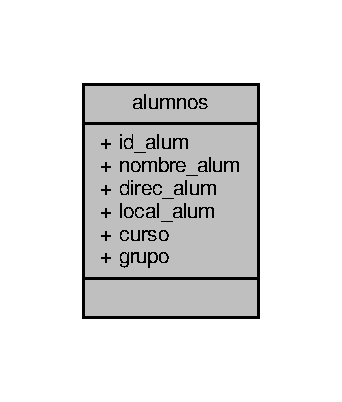
\includegraphics[width=164pt]{structalumnos__coll__graph}
\end{center}
\end{figure}
\subsection*{Public Attributes}
\begin{DoxyCompactItemize}
\item 
char \mbox{\hyperlink{structalumnos_a960ce04015926176477962a5c4199290}{id\+\_\+alum}} \mbox{[}7\mbox{]}
\item 
char \mbox{\hyperlink{structalumnos_a99ddf967c6149106fcdd8d74064dec00}{nombre\+\_\+alum}} \mbox{[}21\mbox{]}
\item 
char \mbox{\hyperlink{structalumnos_aa02cb94abeb6fd35003b880da9e41899}{direc\+\_\+alum}} \mbox{[}31\mbox{]}
\item 
char \mbox{\hyperlink{structalumnos_ac07a90b981cceea8fc4bf627f4126c19}{local\+\_\+alum}} \mbox{[}31\mbox{]}
\item 
char \mbox{\hyperlink{structalumnos_a5cdacbd8eecf8fe90d08936865c1ccf6}{curso}} \mbox{[}31\mbox{]}
\item 
char \mbox{\hyperlink{structalumnos_a1100c8a658fcb00dd7b0a057b1cd0c09}{grupo}} \mbox{[}11\mbox{]}
\end{DoxyCompactItemize}


\subsection{Member Data Documentation}
\mbox{\Hypertarget{structalumnos_a5cdacbd8eecf8fe90d08936865c1ccf6}\label{structalumnos_a5cdacbd8eecf8fe90d08936865c1ccf6}} 
\index{alumnos@{alumnos}!curso@{curso}}
\index{curso@{curso}!alumnos@{alumnos}}
\subsubsection{\texorpdfstring{curso}{curso}}
{\footnotesize\ttfamily char alumnos\+::curso\mbox{[}31\mbox{]}}

\mbox{\Hypertarget{structalumnos_aa02cb94abeb6fd35003b880da9e41899}\label{structalumnos_aa02cb94abeb6fd35003b880da9e41899}} 
\index{alumnos@{alumnos}!direc\+\_\+alum@{direc\+\_\+alum}}
\index{direc\+\_\+alum@{direc\+\_\+alum}!alumnos@{alumnos}}
\subsubsection{\texorpdfstring{direc\+\_\+alum}{direc\_alum}}
{\footnotesize\ttfamily char alumnos\+::direc\+\_\+alum\mbox{[}31\mbox{]}}

\mbox{\Hypertarget{structalumnos_a1100c8a658fcb00dd7b0a057b1cd0c09}\label{structalumnos_a1100c8a658fcb00dd7b0a057b1cd0c09}} 
\index{alumnos@{alumnos}!grupo@{grupo}}
\index{grupo@{grupo}!alumnos@{alumnos}}
\subsubsection{\texorpdfstring{grupo}{grupo}}
{\footnotesize\ttfamily char alumnos\+::grupo\mbox{[}11\mbox{]}}

\mbox{\Hypertarget{structalumnos_a960ce04015926176477962a5c4199290}\label{structalumnos_a960ce04015926176477962a5c4199290}} 
\index{alumnos@{alumnos}!id\+\_\+alum@{id\+\_\+alum}}
\index{id\+\_\+alum@{id\+\_\+alum}!alumnos@{alumnos}}
\subsubsection{\texorpdfstring{id\+\_\+alum}{id\_alum}}
{\footnotesize\ttfamily char alumnos\+::id\+\_\+alum\mbox{[}7\mbox{]}}

\mbox{\Hypertarget{structalumnos_ac07a90b981cceea8fc4bf627f4126c19}\label{structalumnos_ac07a90b981cceea8fc4bf627f4126c19}} 
\index{alumnos@{alumnos}!local\+\_\+alum@{local\+\_\+alum}}
\index{local\+\_\+alum@{local\+\_\+alum}!alumnos@{alumnos}}
\subsubsection{\texorpdfstring{local\+\_\+alum}{local\_alum}}
{\footnotesize\ttfamily char alumnos\+::local\+\_\+alum\mbox{[}31\mbox{]}}

\mbox{\Hypertarget{structalumnos_a99ddf967c6149106fcdd8d74064dec00}\label{structalumnos_a99ddf967c6149106fcdd8d74064dec00}} 
\index{alumnos@{alumnos}!nombre\+\_\+alum@{nombre\+\_\+alum}}
\index{nombre\+\_\+alum@{nombre\+\_\+alum}!alumnos@{alumnos}}
\subsubsection{\texorpdfstring{nombre\+\_\+alum}{nombre\_alum}}
{\footnotesize\ttfamily char alumnos\+::nombre\+\_\+alum\mbox{[}21\mbox{]}}



The documentation for this struct was generated from the following file\+:\begin{DoxyCompactItemize}
\item 
\mbox{\hyperlink{estructuras_8h}{estructuras.\+h}}\end{DoxyCompactItemize}

\hypertarget{structcalificaciones}{}\section{calificaciones Struct Reference}
\label{structcalificaciones}\index{calificaciones@{calificaciones}}


{\ttfamily \#include $<$estructuras.\+h$>$}



Collaboration diagram for calificaciones\+:\nopagebreak
\begin{figure}[H]
\begin{center}
\leavevmode
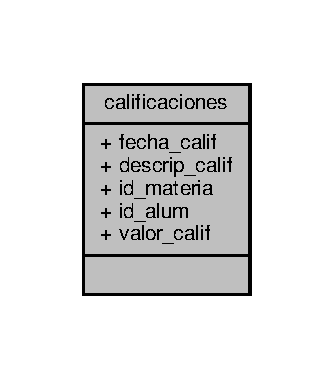
\includegraphics[width=160pt]{structcalificaciones__coll__graph}
\end{center}
\end{figure}
\subsection*{Public Attributes}
\begin{DoxyCompactItemize}
\item 
char \mbox{\hyperlink{structcalificaciones_ae8e8df42a01eb0f08c1e28d0b3b719e4}{fecha\+\_\+calif}} \mbox{[}11\mbox{]}
\item 
char \mbox{\hyperlink{structcalificaciones_a4da5aee40f1cbe0d2cf2a19a2d62cd90}{descrip\+\_\+calif}} \mbox{[}31\mbox{]}
\item 
char \mbox{\hyperlink{structcalificaciones_ab3e1ecafa94442f9ea47eee45208b08b}{id\+\_\+materia}} \mbox{[}5\mbox{]}
\item 
char \mbox{\hyperlink{structcalificaciones_a25420b2789fc7452fd044ca3b318ed92}{id\+\_\+alum}} \mbox{[}7\mbox{]}
\item 
int \mbox{\hyperlink{structcalificaciones_af79ae6ed55e0fc1bfd9746b78b75fa6c}{valor\+\_\+calif}}
\end{DoxyCompactItemize}


\subsection{Member Data Documentation}
\mbox{\Hypertarget{structcalificaciones_a4da5aee40f1cbe0d2cf2a19a2d62cd90}\label{structcalificaciones_a4da5aee40f1cbe0d2cf2a19a2d62cd90}} 
\index{calificaciones@{calificaciones}!descrip\+\_\+calif@{descrip\+\_\+calif}}
\index{descrip\+\_\+calif@{descrip\+\_\+calif}!calificaciones@{calificaciones}}
\subsubsection{\texorpdfstring{descrip\+\_\+calif}{descrip\_calif}}
{\footnotesize\ttfamily char calificaciones\+::descrip\+\_\+calif\mbox{[}31\mbox{]}}

\mbox{\Hypertarget{structcalificaciones_ae8e8df42a01eb0f08c1e28d0b3b719e4}\label{structcalificaciones_ae8e8df42a01eb0f08c1e28d0b3b719e4}} 
\index{calificaciones@{calificaciones}!fecha\+\_\+calif@{fecha\+\_\+calif}}
\index{fecha\+\_\+calif@{fecha\+\_\+calif}!calificaciones@{calificaciones}}
\subsubsection{\texorpdfstring{fecha\+\_\+calif}{fecha\_calif}}
{\footnotesize\ttfamily char calificaciones\+::fecha\+\_\+calif\mbox{[}11\mbox{]}}

\mbox{\Hypertarget{structcalificaciones_a25420b2789fc7452fd044ca3b318ed92}\label{structcalificaciones_a25420b2789fc7452fd044ca3b318ed92}} 
\index{calificaciones@{calificaciones}!id\+\_\+alum@{id\+\_\+alum}}
\index{id\+\_\+alum@{id\+\_\+alum}!calificaciones@{calificaciones}}
\subsubsection{\texorpdfstring{id\+\_\+alum}{id\_alum}}
{\footnotesize\ttfamily char calificaciones\+::id\+\_\+alum\mbox{[}7\mbox{]}}

\mbox{\Hypertarget{structcalificaciones_ab3e1ecafa94442f9ea47eee45208b08b}\label{structcalificaciones_ab3e1ecafa94442f9ea47eee45208b08b}} 
\index{calificaciones@{calificaciones}!id\+\_\+materia@{id\+\_\+materia}}
\index{id\+\_\+materia@{id\+\_\+materia}!calificaciones@{calificaciones}}
\subsubsection{\texorpdfstring{id\+\_\+materia}{id\_materia}}
{\footnotesize\ttfamily char calificaciones\+::id\+\_\+materia\mbox{[}5\mbox{]}}

\mbox{\Hypertarget{structcalificaciones_af79ae6ed55e0fc1bfd9746b78b75fa6c}\label{structcalificaciones_af79ae6ed55e0fc1bfd9746b78b75fa6c}} 
\index{calificaciones@{calificaciones}!valor\+\_\+calif@{valor\+\_\+calif}}
\index{valor\+\_\+calif@{valor\+\_\+calif}!calificaciones@{calificaciones}}
\subsubsection{\texorpdfstring{valor\+\_\+calif}{valor\_calif}}
{\footnotesize\ttfamily int calificaciones\+::valor\+\_\+calif}



The documentation for this struct was generated from the following file\+:\begin{DoxyCompactItemize}
\item 
\mbox{\hyperlink{estructuras_8h}{estructuras.\+h}}\end{DoxyCompactItemize}

\hypertarget{structfaltas}{}\section{Referencia de la Estructura faltas}
\label{structfaltas}\index{faltas@{faltas}}


{\ttfamily \#include $<$estructuras.\+h$>$}

\subsection*{Campos de datos}
\begin{DoxyCompactItemize}
\item 
char \mbox{\hyperlink{structfaltas_af129c434d523f950657f329ee13598b5}{fecha\+\_\+falta}} \mbox{[}11\mbox{]}
\item 
int \mbox{\hyperlink{structfaltas_a896bc2033259f82ae633907298b3a65d}{hora\+\_\+falta}}
\item 
char \mbox{\hyperlink{structfaltas_a4c7f9998f31cf6251caa0216c7639b24}{descrip\+\_\+falta}} \mbox{[}31\mbox{]}
\item 
char \mbox{\hyperlink{structfaltas_abcd66e5b1e7f572c68cfc2d860289ee3}{estado\+\_\+falta}} \mbox{[}14\mbox{]}
\item 
char \mbox{\hyperlink{structfaltas_adf78bf54f25af0e394df78fc3ef765fa}{id\+\_\+alum}} \mbox{[}7\mbox{]}
\end{DoxyCompactItemize}


\subsection{Descripción detallada}


Definición en la línea 48 del archivo estructuras.\+h.



\subsection{Documentación de los campos}
\mbox{\Hypertarget{structfaltas_a4c7f9998f31cf6251caa0216c7639b24}\label{structfaltas_a4c7f9998f31cf6251caa0216c7639b24}} 
\index{faltas@{faltas}!descrip\+\_\+falta@{descrip\+\_\+falta}}
\index{descrip\+\_\+falta@{descrip\+\_\+falta}!faltas@{faltas}}
\subsubsection{\texorpdfstring{descrip\+\_\+falta}{descrip\_falta}}
{\footnotesize\ttfamily char faltas\+::descrip\+\_\+falta\mbox{[}31\mbox{]}}



Definición en la línea 51 del archivo estructuras.\+h.

\mbox{\Hypertarget{structfaltas_abcd66e5b1e7f572c68cfc2d860289ee3}\label{structfaltas_abcd66e5b1e7f572c68cfc2d860289ee3}} 
\index{faltas@{faltas}!estado\+\_\+falta@{estado\+\_\+falta}}
\index{estado\+\_\+falta@{estado\+\_\+falta}!faltas@{faltas}}
\subsubsection{\texorpdfstring{estado\+\_\+falta}{estado\_falta}}
{\footnotesize\ttfamily char faltas\+::estado\+\_\+falta\mbox{[}14\mbox{]}}



Definición en la línea 52 del archivo estructuras.\+h.

\mbox{\Hypertarget{structfaltas_af129c434d523f950657f329ee13598b5}\label{structfaltas_af129c434d523f950657f329ee13598b5}} 
\index{faltas@{faltas}!fecha\+\_\+falta@{fecha\+\_\+falta}}
\index{fecha\+\_\+falta@{fecha\+\_\+falta}!faltas@{faltas}}
\subsubsection{\texorpdfstring{fecha\+\_\+falta}{fecha\_falta}}
{\footnotesize\ttfamily char faltas\+::fecha\+\_\+falta\mbox{[}11\mbox{]}}



Definición en la línea 49 del archivo estructuras.\+h.

\mbox{\Hypertarget{structfaltas_a896bc2033259f82ae633907298b3a65d}\label{structfaltas_a896bc2033259f82ae633907298b3a65d}} 
\index{faltas@{faltas}!hora\+\_\+falta@{hora\+\_\+falta}}
\index{hora\+\_\+falta@{hora\+\_\+falta}!faltas@{faltas}}
\subsubsection{\texorpdfstring{hora\+\_\+falta}{hora\_falta}}
{\footnotesize\ttfamily int faltas\+::hora\+\_\+falta}



Definición en la línea 50 del archivo estructuras.\+h.

\mbox{\Hypertarget{structfaltas_adf78bf54f25af0e394df78fc3ef765fa}\label{structfaltas_adf78bf54f25af0e394df78fc3ef765fa}} 
\index{faltas@{faltas}!id\+\_\+alum@{id\+\_\+alum}}
\index{id\+\_\+alum@{id\+\_\+alum}!faltas@{faltas}}
\subsubsection{\texorpdfstring{id\+\_\+alum}{id\_alum}}
{\footnotesize\ttfamily char faltas\+::id\+\_\+alum\mbox{[}7\mbox{]}}



Definición en la línea 53 del archivo estructuras.\+h.



La documentación para esta estructura fue generada a partir del siguiente fichero\+:\begin{DoxyCompactItemize}
\item 
\mbox{\hyperlink{estructuras_8h}{estructuras.\+h}}\end{DoxyCompactItemize}

\hypertarget{structhorarios}{}\section{horarios Struct Reference}
\label{structhorarios}\index{horarios@{horarios}}


{\ttfamily \#include $<$estructuras.\+h$>$}



Collaboration diagram for horarios\+:\nopagebreak
\begin{figure}[H]
\begin{center}
\leavevmode
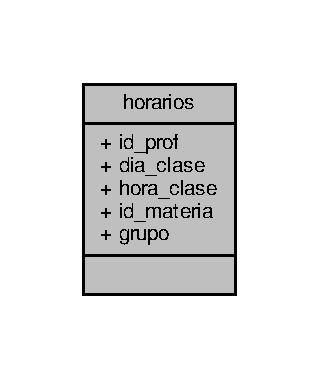
\includegraphics[width=153pt]{structhorarios__coll__graph}
\end{center}
\end{figure}
\subsection*{Public Attributes}
\begin{DoxyCompactItemize}
\item 
char \mbox{\hyperlink{structhorarios_a10531356ac4d127379c96ad1006873f8}{id\+\_\+prof}} \mbox{[}4\mbox{]}
\item 
int \mbox{\hyperlink{structhorarios_a514443404c267c542497e9c22f6d3e25}{dia\+\_\+clase}}
\item 
int \mbox{\hyperlink{structhorarios_a5ed630f7244ecfbe4c29f08ffb009472}{hora\+\_\+clase}}
\item 
char \mbox{\hyperlink{structhorarios_adbe2c73c92199ce4ac6e03b7cdbe9b72}{id\+\_\+materia}} \mbox{[}5\mbox{]}
\item 
char \mbox{\hyperlink{structhorarios_a435f7d8029b65cba591011c6d86ce284}{grupo}} \mbox{[}500\mbox{]}
\end{DoxyCompactItemize}


\subsection{Member Data Documentation}
\mbox{\Hypertarget{structhorarios_a514443404c267c542497e9c22f6d3e25}\label{structhorarios_a514443404c267c542497e9c22f6d3e25}} 
\index{horarios@{horarios}!dia\+\_\+clase@{dia\+\_\+clase}}
\index{dia\+\_\+clase@{dia\+\_\+clase}!horarios@{horarios}}
\subsubsection{\texorpdfstring{dia\+\_\+clase}{dia\_clase}}
{\footnotesize\ttfamily int horarios\+::dia\+\_\+clase}

\mbox{\Hypertarget{structhorarios_a435f7d8029b65cba591011c6d86ce284}\label{structhorarios_a435f7d8029b65cba591011c6d86ce284}} 
\index{horarios@{horarios}!grupo@{grupo}}
\index{grupo@{grupo}!horarios@{horarios}}
\subsubsection{\texorpdfstring{grupo}{grupo}}
{\footnotesize\ttfamily char horarios\+::grupo\mbox{[}500\mbox{]}}

\mbox{\Hypertarget{structhorarios_a5ed630f7244ecfbe4c29f08ffb009472}\label{structhorarios_a5ed630f7244ecfbe4c29f08ffb009472}} 
\index{horarios@{horarios}!hora\+\_\+clase@{hora\+\_\+clase}}
\index{hora\+\_\+clase@{hora\+\_\+clase}!horarios@{horarios}}
\subsubsection{\texorpdfstring{hora\+\_\+clase}{hora\_clase}}
{\footnotesize\ttfamily int horarios\+::hora\+\_\+clase}

\mbox{\Hypertarget{structhorarios_adbe2c73c92199ce4ac6e03b7cdbe9b72}\label{structhorarios_adbe2c73c92199ce4ac6e03b7cdbe9b72}} 
\index{horarios@{horarios}!id\+\_\+materia@{id\+\_\+materia}}
\index{id\+\_\+materia@{id\+\_\+materia}!horarios@{horarios}}
\subsubsection{\texorpdfstring{id\+\_\+materia}{id\_materia}}
{\footnotesize\ttfamily char horarios\+::id\+\_\+materia\mbox{[}5\mbox{]}}

\mbox{\Hypertarget{structhorarios_a10531356ac4d127379c96ad1006873f8}\label{structhorarios_a10531356ac4d127379c96ad1006873f8}} 
\index{horarios@{horarios}!id\+\_\+prof@{id\+\_\+prof}}
\index{id\+\_\+prof@{id\+\_\+prof}!horarios@{horarios}}
\subsubsection{\texorpdfstring{id\+\_\+prof}{id\_prof}}
{\footnotesize\ttfamily char horarios\+::id\+\_\+prof\mbox{[}4\mbox{]}}



The documentation for this struct was generated from the following file\+:\begin{DoxyCompactItemize}
\item 
\mbox{\hyperlink{estructuras_8h}{estructuras.\+h}}\end{DoxyCompactItemize}

\hypertarget{structmaterias}{}\section{Referencia de la Estructura materias}
\label{structmaterias}\index{materias@{materias}}


{\ttfamily \#include $<$estructuras.\+h$>$}

\subsection*{Campos de datos}
\begin{DoxyCompactItemize}
\item 
char \mbox{\hyperlink{structmaterias_ae285579bc06c3da15f087e1c1b829068}{id\+\_\+materia}} \mbox{[}5\mbox{]}
\item 
char \mbox{\hyperlink{structmaterias_a5d39a4c56dcd41b1cdc9873c5873400e}{nombre\+\_\+materia}} \mbox{[}100\mbox{]}
\item 
char \mbox{\hyperlink{structmaterias_a3cbb90c8931ebfaa78e3c26679845746}{abrev\+\_\+materia}} \mbox{[}10\mbox{]}
\end{DoxyCompactItemize}


\subsection{Descripción detallada}


Definición en la línea 23 del archivo estructuras.\+h.



\subsection{Documentación de los campos}
\mbox{\Hypertarget{structmaterias_a3cbb90c8931ebfaa78e3c26679845746}\label{structmaterias_a3cbb90c8931ebfaa78e3c26679845746}} 
\index{materias@{materias}!abrev\+\_\+materia@{abrev\+\_\+materia}}
\index{abrev\+\_\+materia@{abrev\+\_\+materia}!materias@{materias}}
\subsubsection{\texorpdfstring{abrev\+\_\+materia}{abrev\_materia}}
{\footnotesize\ttfamily char materias\+::abrev\+\_\+materia\mbox{[}10\mbox{]}}



Definición en la línea 26 del archivo estructuras.\+h.

\mbox{\Hypertarget{structmaterias_ae285579bc06c3da15f087e1c1b829068}\label{structmaterias_ae285579bc06c3da15f087e1c1b829068}} 
\index{materias@{materias}!id\+\_\+materia@{id\+\_\+materia}}
\index{id\+\_\+materia@{id\+\_\+materia}!materias@{materias}}
\subsubsection{\texorpdfstring{id\+\_\+materia}{id\_materia}}
{\footnotesize\ttfamily char materias\+::id\+\_\+materia\mbox{[}5\mbox{]}}



Definición en la línea 24 del archivo estructuras.\+h.

\mbox{\Hypertarget{structmaterias_a5d39a4c56dcd41b1cdc9873c5873400e}\label{structmaterias_a5d39a4c56dcd41b1cdc9873c5873400e}} 
\index{materias@{materias}!nombre\+\_\+materia@{nombre\+\_\+materia}}
\index{nombre\+\_\+materia@{nombre\+\_\+materia}!materias@{materias}}
\subsubsection{\texorpdfstring{nombre\+\_\+materia}{nombre\_materia}}
{\footnotesize\ttfamily char materias\+::nombre\+\_\+materia\mbox{[}100\mbox{]}}



Definición en la línea 25 del archivo estructuras.\+h.



La documentación para esta estructura fue generada a partir del siguiente fichero\+:\begin{DoxyCompactItemize}
\item 
\mbox{\hyperlink{estructuras_8h}{estructuras.\+h}}\end{DoxyCompactItemize}

\hypertarget{structmatriculas}{}\section{matriculas Struct Reference}
\label{structmatriculas}\index{matriculas@{matriculas}}


{\ttfamily \#include $<$estructuras.\+h$>$}



Collaboration diagram for matriculas\+:\nopagebreak
\begin{figure}[H]
\begin{center}
\leavevmode
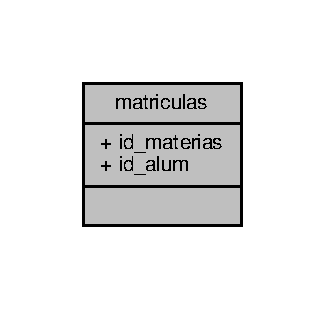
\includegraphics[width=156pt]{structmatriculas__coll__graph}
\end{center}
\end{figure}
\subsection*{Public Attributes}
\begin{DoxyCompactItemize}
\item 
char \mbox{\hyperlink{structmatriculas_a6433d557ea453570a08401f83be557d0}{id\+\_\+materias}} \mbox{[}5\mbox{]}
\item 
char \mbox{\hyperlink{structmatriculas_aff338fa16ed08905b6e2b214d743fb41}{id\+\_\+alum}} \mbox{[}7\mbox{]}
\end{DoxyCompactItemize}


\subsection{Member Data Documentation}
\mbox{\Hypertarget{structmatriculas_aff338fa16ed08905b6e2b214d743fb41}\label{structmatriculas_aff338fa16ed08905b6e2b214d743fb41}} 
\index{matriculas@{matriculas}!id\+\_\+alum@{id\+\_\+alum}}
\index{id\+\_\+alum@{id\+\_\+alum}!matriculas@{matriculas}}
\subsubsection{\texorpdfstring{id\+\_\+alum}{id\_alum}}
{\footnotesize\ttfamily char matriculas\+::id\+\_\+alum\mbox{[}7\mbox{]}}

\mbox{\Hypertarget{structmatriculas_a6433d557ea453570a08401f83be557d0}\label{structmatriculas_a6433d557ea453570a08401f83be557d0}} 
\index{matriculas@{matriculas}!id\+\_\+materias@{id\+\_\+materias}}
\index{id\+\_\+materias@{id\+\_\+materias}!matriculas@{matriculas}}
\subsubsection{\texorpdfstring{id\+\_\+materias}{id\_materias}}
{\footnotesize\ttfamily char matriculas\+::id\+\_\+materias\mbox{[}5\mbox{]}}



The documentation for this struct was generated from the following file\+:\begin{DoxyCompactItemize}
\item 
\mbox{\hyperlink{estructuras_8h}{estructuras.\+h}}\end{DoxyCompactItemize}

\hypertarget{structusuarios}{}\section{usuarios Struct Reference}
\label{structusuarios}\index{usuarios@{usuarios}}


{\ttfamily \#include $<$estructuras.\+h$>$}



Collaboration diagram for usuarios\+:\nopagebreak
\begin{figure}[H]
\begin{center}
\leavevmode
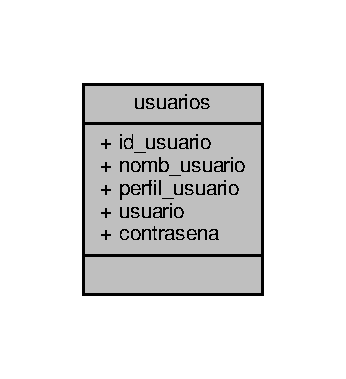
\includegraphics[width=166pt]{structusuarios__coll__graph}
\end{center}
\end{figure}
\subsection*{Public Attributes}
\begin{DoxyCompactItemize}
\item 
char \mbox{\hyperlink{structusuarios_a5090e2f56888f1a9873bd9ed35bf46d3}{id\+\_\+usuario}} \mbox{[}4\mbox{]}
\item 
char \mbox{\hyperlink{structusuarios_acf2d33748c720f047d2a0e512e187fd5}{nomb\+\_\+usuario}} \mbox{[}21\mbox{]}
\item 
char \mbox{\hyperlink{structusuarios_afe590222f989c0e30b72bbc0014868cc}{perfil\+\_\+usuario}} \mbox{[}14\mbox{]}
\item 
char \mbox{\hyperlink{structusuarios_a3330601c31921ae73c6fa7551a68a0da}{usuario}} \mbox{[}21\mbox{]}
\item 
char \mbox{\hyperlink{structusuarios_a0689cc96bd888f121b04e5c43d47a028}{contrasena}} \mbox{[}9\mbox{]}
\end{DoxyCompactItemize}


\subsection{Member Data Documentation}
\mbox{\Hypertarget{structusuarios_a0689cc96bd888f121b04e5c43d47a028}\label{structusuarios_a0689cc96bd888f121b04e5c43d47a028}} 
\index{usuarios@{usuarios}!contrasena@{contrasena}}
\index{contrasena@{contrasena}!usuarios@{usuarios}}
\subsubsection{\texorpdfstring{contrasena}{contrasena}}
{\footnotesize\ttfamily char usuarios\+::contrasena\mbox{[}9\mbox{]}}

\mbox{\Hypertarget{structusuarios_a5090e2f56888f1a9873bd9ed35bf46d3}\label{structusuarios_a5090e2f56888f1a9873bd9ed35bf46d3}} 
\index{usuarios@{usuarios}!id\+\_\+usuario@{id\+\_\+usuario}}
\index{id\+\_\+usuario@{id\+\_\+usuario}!usuarios@{usuarios}}
\subsubsection{\texorpdfstring{id\+\_\+usuario}{id\_usuario}}
{\footnotesize\ttfamily char usuarios\+::id\+\_\+usuario\mbox{[}4\mbox{]}}

\mbox{\Hypertarget{structusuarios_acf2d33748c720f047d2a0e512e187fd5}\label{structusuarios_acf2d33748c720f047d2a0e512e187fd5}} 
\index{usuarios@{usuarios}!nomb\+\_\+usuario@{nomb\+\_\+usuario}}
\index{nomb\+\_\+usuario@{nomb\+\_\+usuario}!usuarios@{usuarios}}
\subsubsection{\texorpdfstring{nomb\+\_\+usuario}{nomb\_usuario}}
{\footnotesize\ttfamily char usuarios\+::nomb\+\_\+usuario\mbox{[}21\mbox{]}}

\mbox{\Hypertarget{structusuarios_afe590222f989c0e30b72bbc0014868cc}\label{structusuarios_afe590222f989c0e30b72bbc0014868cc}} 
\index{usuarios@{usuarios}!perfil\+\_\+usuario@{perfil\+\_\+usuario}}
\index{perfil\+\_\+usuario@{perfil\+\_\+usuario}!usuarios@{usuarios}}
\subsubsection{\texorpdfstring{perfil\+\_\+usuario}{perfil\_usuario}}
{\footnotesize\ttfamily char usuarios\+::perfil\+\_\+usuario\mbox{[}14\mbox{]}}

\mbox{\Hypertarget{structusuarios_a3330601c31921ae73c6fa7551a68a0da}\label{structusuarios_a3330601c31921ae73c6fa7551a68a0da}} 
\index{usuarios@{usuarios}!usuario@{usuario}}
\index{usuario@{usuario}!usuarios@{usuarios}}
\subsubsection{\texorpdfstring{usuario}{usuario}}
{\footnotesize\ttfamily char usuarios\+::usuario\mbox{[}21\mbox{]}}



The documentation for this struct was generated from the following file\+:\begin{DoxyCompactItemize}
\item 
\mbox{\hyperlink{estructuras_8h}{estructuras.\+h}}\end{DoxyCompactItemize}

\chapter{Documentación de archivos}
\hypertarget{alumnos_8c}{}\section{alumnos.\+c File Reference}
\label{alumnos_8c}\index{alumnos.\+c@{alumnos.\+c}}
{\ttfamily \#include $<$stdio.\+h$>$}\newline
{\ttfamily \#include $<$stdlib.\+h$>$}\newline
{\ttfamily \#include $<$string.\+h$>$}\newline
{\ttfamily \#include \char`\"{}estructuras.\+h\char`\"{}}\newline
{\ttfamily \#include \char`\"{}alumnos.\+h\char`\"{}}\newline
Include dependency graph for alumnos.\+c\+:\nopagebreak
\begin{figure}[H]
\begin{center}
\leavevmode
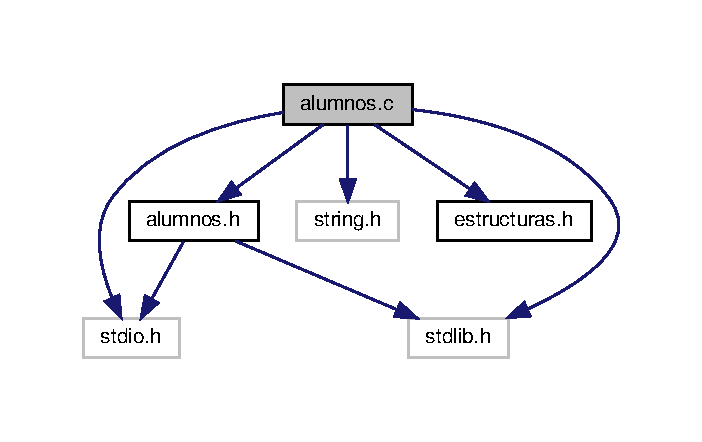
\includegraphics[width=337pt]{alumnos_8c__incl}
\end{center}
\end{figure}
This graph shows which files directly or indirectly include this file\+:\nopagebreak
\begin{figure}[H]
\begin{center}
\leavevmode
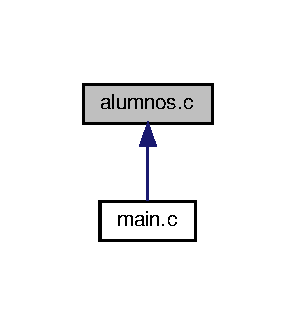
\includegraphics[width=142pt]{alumnos_8c__dep__incl}
\end{center}
\end{figure}
\subsection*{Functions}
\begin{DoxyCompactItemize}
\item 
void \mbox{\hyperlink{alumnos_8c_aa0ecdc5d299fcbde0eb715eb564f026f}{quitar\+\_\+saltosA}} (char $\ast$)
\item 
char $\ast$ \mbox{\hyperlink{alumnos_8c_abac62976847524d39299f3c5cb0f7bec}{leer\+\_\+campo\+\_\+A}} (int, char $\ast$)
\item 
void \mbox{\hyperlink{alumnos_8c_a23b200c89a3f9cd634292b6badc924bc}{Modificar\+\_\+\+Alumno\+\_\+ficha}} (\mbox{\hyperlink{structalumnos}{alumnos}} $\ast$, int)
\item 
\mbox{\hyperlink{structalumnos}{alumnos}} $\ast$ \mbox{\hyperlink{alumnos_8c_acb60a266abe9b3631929cafc7077ee56}{Carga\+\_\+\+Alumno}} ()
\item 
void \mbox{\hyperlink{alumnos_8c_a78832a2b6a02da48d43240f1ae7a273e}{menu\+\_\+alumnos}} (\mbox{\hyperlink{structalumnos}{alumnos}} $\ast$\mbox{\hyperlink{main_8c_a074bcb9e388f87c39fbb2fba8788bd46}{arr\+\_\+alumnos}})
\item 
char $\ast$ \mbox{\hyperlink{alumnos_8c_a0ccfda8635c0219cd8397f0c76be0aa5}{listar\+\_\+alumnos\+\_\+prof}} (\mbox{\hyperlink{structalumnos}{alumnos}} $\ast$List\+\_\+\+Alumno, char $\ast$id)
\item 
void \mbox{\hyperlink{alumnos_8c_a8fd4a049c61775b5008c0644d3125c1a}{ficha\+\_\+alum}} (\mbox{\hyperlink{structalumnos}{alumnos}} $\ast$List\+\_\+\+Alumno, char $\ast$cod)
\item 
void \mbox{\hyperlink{alumnos_8c_afe7aba672f2872504eb20064e4d3fa8f}{Anadir\+\_\+\+Alumno}} (\mbox{\hyperlink{structalumnos}{alumnos}} $\ast$List\+\_\+\+Alumno)
\item 
void \mbox{\hyperlink{alumnos_8c_ac1b962c53e14b0375e64a44ebdcc38fa}{Listar\+\_\+\+Alumno}} (\mbox{\hyperlink{structalumnos}{alumnos}} $\ast$List\+\_\+\+Alumno)
\item 
void \mbox{\hyperlink{alumnos_8c_a8dcb4e8881eb636706040c9e73d79ba4}{Modificar\+\_\+\+Alumno}} (\mbox{\hyperlink{structalumnos}{alumnos}} $\ast$List\+\_\+\+Alumno)
\item 
void \mbox{\hyperlink{alumnos_8c_ae9eedadeae49bfc6516ff6b4bb1b1e71}{Baja\+\_\+\+Alumno}} (\mbox{\hyperlink{structalumnos}{alumnos}} $\ast$List\+\_\+\+Alumno)
\item 
void \mbox{\hyperlink{alumnos_8c_a4fe99b2e3623b105ff15cf21bfb0bf42}{Guardar\+\_\+\+Alumno}} (\mbox{\hyperlink{structalumnos}{alumnos}} $\ast$List\+\_\+\+Alumno)
\end{DoxyCompactItemize}
\subsection*{Variables}
\begin{DoxyCompactItemize}
\item 
int \mbox{\hyperlink{alumnos_8c_a64e3b8d4f87de890cc5ee7edee65b616}{conta}} =0
\end{DoxyCompactItemize}


\subsection{Function Documentation}
\mbox{\Hypertarget{alumnos_8c_afe7aba672f2872504eb20064e4d3fa8f}\label{alumnos_8c_afe7aba672f2872504eb20064e4d3fa8f}} 
\index{alumnos.\+c@{alumnos.\+c}!Anadir\+\_\+\+Alumno@{Anadir\+\_\+\+Alumno}}
\index{Anadir\+\_\+\+Alumno@{Anadir\+\_\+\+Alumno}!alumnos.\+c@{alumnos.\+c}}
\subsubsection{\texorpdfstring{Anadir\+\_\+\+Alumno()}{Anadir\_Alumno()}}
{\footnotesize\ttfamily void Anadir\+\_\+\+Alumno (\begin{DoxyParamCaption}\item[{\mbox{\hyperlink{structalumnos}{alumnos}} $\ast$}]{List\+\_\+\+Alumno }\end{DoxyParamCaption})}

Here is the call graph for this function\+:\nopagebreak
\begin{figure}[H]
\begin{center}
\leavevmode
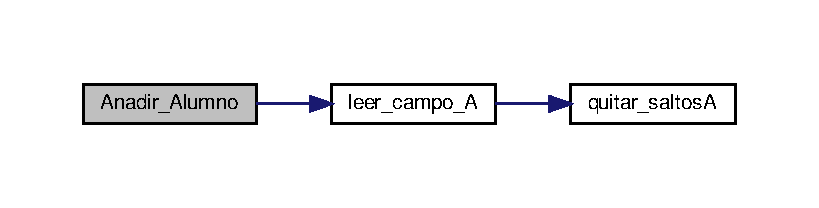
\includegraphics[width=350pt]{alumnos_8c_afe7aba672f2872504eb20064e4d3fa8f_cgraph}
\end{center}
\end{figure}
Here is the caller graph for this function\+:\nopagebreak
\begin{figure}[H]
\begin{center}
\leavevmode
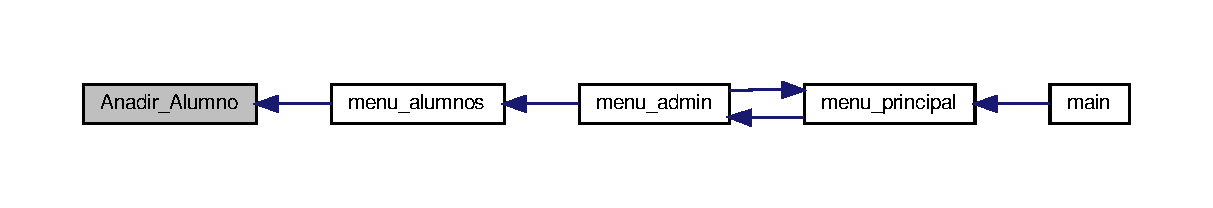
\includegraphics[width=350pt]{alumnos_8c_afe7aba672f2872504eb20064e4d3fa8f_icgraph}
\end{center}
\end{figure}
\mbox{\Hypertarget{alumnos_8c_ae9eedadeae49bfc6516ff6b4bb1b1e71}\label{alumnos_8c_ae9eedadeae49bfc6516ff6b4bb1b1e71}} 
\index{alumnos.\+c@{alumnos.\+c}!Baja\+\_\+\+Alumno@{Baja\+\_\+\+Alumno}}
\index{Baja\+\_\+\+Alumno@{Baja\+\_\+\+Alumno}!alumnos.\+c@{alumnos.\+c}}
\subsubsection{\texorpdfstring{Baja\+\_\+\+Alumno()}{Baja\_Alumno()}}
{\footnotesize\ttfamily void Baja\+\_\+\+Alumno (\begin{DoxyParamCaption}\item[{\mbox{\hyperlink{structalumnos}{alumnos}} $\ast$}]{List\+\_\+\+Alumno }\end{DoxyParamCaption})}

Here is the call graph for this function\+:\nopagebreak
\begin{figure}[H]
\begin{center}
\leavevmode
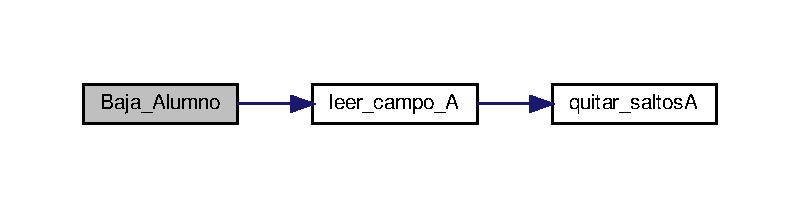
\includegraphics[width=350pt]{alumnos_8c_ae9eedadeae49bfc6516ff6b4bb1b1e71_cgraph}
\end{center}
\end{figure}
Here is the caller graph for this function\+:\nopagebreak
\begin{figure}[H]
\begin{center}
\leavevmode
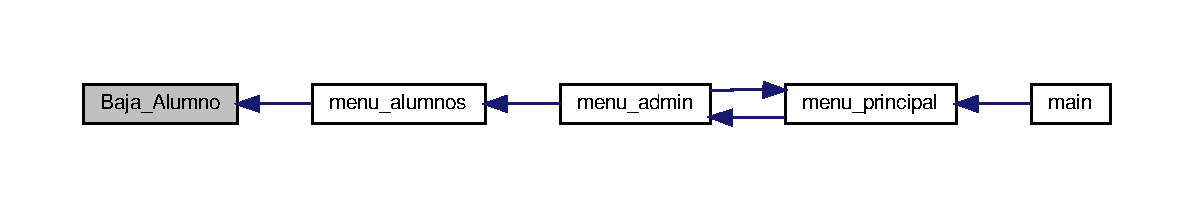
\includegraphics[width=350pt]{alumnos_8c_ae9eedadeae49bfc6516ff6b4bb1b1e71_icgraph}
\end{center}
\end{figure}
\mbox{\Hypertarget{alumnos_8c_acb60a266abe9b3631929cafc7077ee56}\label{alumnos_8c_acb60a266abe9b3631929cafc7077ee56}} 
\index{alumnos.\+c@{alumnos.\+c}!Carga\+\_\+\+Alumno@{Carga\+\_\+\+Alumno}}
\index{Carga\+\_\+\+Alumno@{Carga\+\_\+\+Alumno}!alumnos.\+c@{alumnos.\+c}}
\subsubsection{\texorpdfstring{Carga\+\_\+\+Alumno()}{Carga\_Alumno()}}
{\footnotesize\ttfamily \mbox{\hyperlink{structalumnos}{alumnos}}$\ast$ Carga\+\_\+\+Alumno (\begin{DoxyParamCaption}{ }\end{DoxyParamCaption})}

Here is the caller graph for this function\+:\nopagebreak
\begin{figure}[H]
\begin{center}
\leavevmode
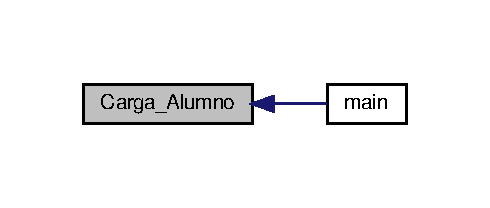
\includegraphics[width=235pt]{alumnos_8c_acb60a266abe9b3631929cafc7077ee56_icgraph}
\end{center}
\end{figure}
\mbox{\Hypertarget{alumnos_8c_a8fd4a049c61775b5008c0644d3125c1a}\label{alumnos_8c_a8fd4a049c61775b5008c0644d3125c1a}} 
\index{alumnos.\+c@{alumnos.\+c}!ficha\+\_\+alum@{ficha\+\_\+alum}}
\index{ficha\+\_\+alum@{ficha\+\_\+alum}!alumnos.\+c@{alumnos.\+c}}
\subsubsection{\texorpdfstring{ficha\+\_\+alum()}{ficha\_alum()}}
{\footnotesize\ttfamily void ficha\+\_\+alum (\begin{DoxyParamCaption}\item[{\mbox{\hyperlink{structalumnos}{alumnos}} $\ast$}]{List\+\_\+\+Alumno,  }\item[{char $\ast$}]{cod }\end{DoxyParamCaption})}

Here is the call graph for this function\+:\nopagebreak
\begin{figure}[H]
\begin{center}
\leavevmode
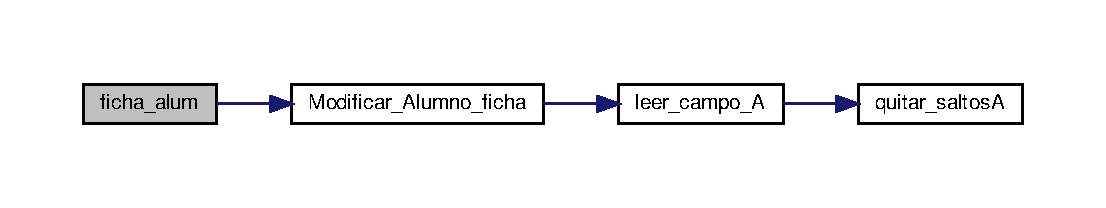
\includegraphics[width=350pt]{alumnos_8c_a8fd4a049c61775b5008c0644d3125c1a_cgraph}
\end{center}
\end{figure}
Here is the caller graph for this function\+:\nopagebreak
\begin{figure}[H]
\begin{center}
\leavevmode
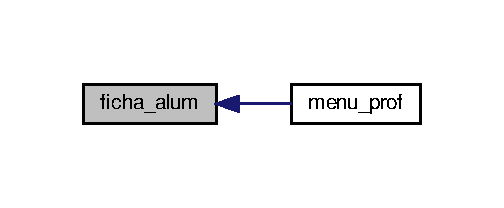
\includegraphics[width=242pt]{alumnos_8c_a8fd4a049c61775b5008c0644d3125c1a_icgraph}
\end{center}
\end{figure}
\mbox{\Hypertarget{alumnos_8c_a4fe99b2e3623b105ff15cf21bfb0bf42}\label{alumnos_8c_a4fe99b2e3623b105ff15cf21bfb0bf42}} 
\index{alumnos.\+c@{alumnos.\+c}!Guardar\+\_\+\+Alumno@{Guardar\+\_\+\+Alumno}}
\index{Guardar\+\_\+\+Alumno@{Guardar\+\_\+\+Alumno}!alumnos.\+c@{alumnos.\+c}}
\subsubsection{\texorpdfstring{Guardar\+\_\+\+Alumno()}{Guardar\_Alumno()}}
{\footnotesize\ttfamily void Guardar\+\_\+\+Alumno (\begin{DoxyParamCaption}\item[{\mbox{\hyperlink{structalumnos}{alumnos}} $\ast$}]{List\+\_\+\+Alumno }\end{DoxyParamCaption})}

Here is the caller graph for this function\+:\nopagebreak
\begin{figure}[H]
\begin{center}
\leavevmode
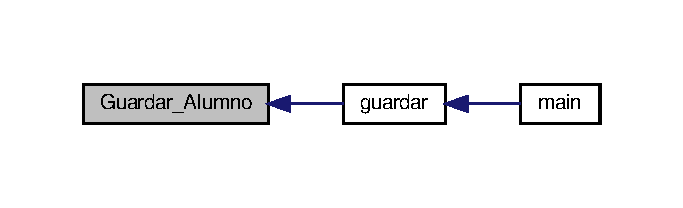
\includegraphics[width=328pt]{alumnos_8c_a4fe99b2e3623b105ff15cf21bfb0bf42_icgraph}
\end{center}
\end{figure}
\mbox{\Hypertarget{alumnos_8c_abac62976847524d39299f3c5cb0f7bec}\label{alumnos_8c_abac62976847524d39299f3c5cb0f7bec}} 
\index{alumnos.\+c@{alumnos.\+c}!leer\+\_\+campo\+\_\+A@{leer\+\_\+campo\+\_\+A}}
\index{leer\+\_\+campo\+\_\+A@{leer\+\_\+campo\+\_\+A}!alumnos.\+c@{alumnos.\+c}}
\subsubsection{\texorpdfstring{leer\+\_\+campo\+\_\+\+A()}{leer\_campo\_A()}}
{\footnotesize\ttfamily char $\ast$ leer\+\_\+campo\+\_\+A (\begin{DoxyParamCaption}\item[{int}]{largo,  }\item[{char $\ast$}]{titulo }\end{DoxyParamCaption})}

Here is the call graph for this function\+:\nopagebreak
\begin{figure}[H]
\begin{center}
\leavevmode
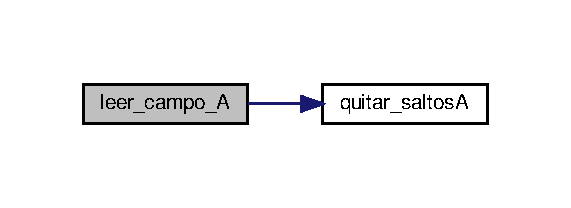
\includegraphics[width=274pt]{alumnos_8c_abac62976847524d39299f3c5cb0f7bec_cgraph}
\end{center}
\end{figure}
Here is the caller graph for this function\+:\nopagebreak
\begin{figure}[H]
\begin{center}
\leavevmode
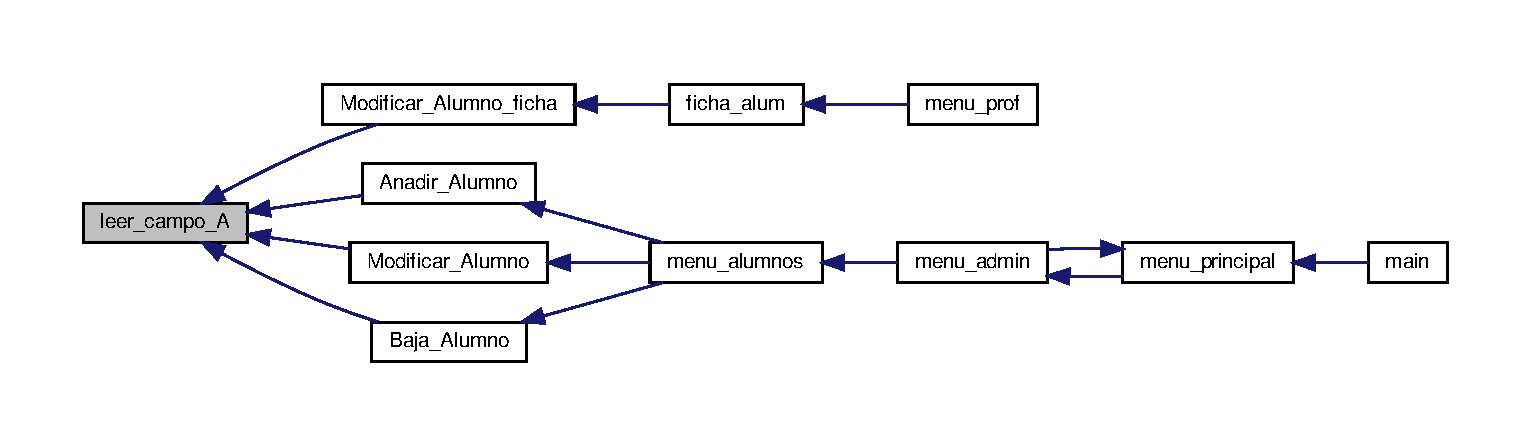
\includegraphics[width=350pt]{alumnos_8c_abac62976847524d39299f3c5cb0f7bec_icgraph}
\end{center}
\end{figure}
\mbox{\Hypertarget{alumnos_8c_ac1b962c53e14b0375e64a44ebdcc38fa}\label{alumnos_8c_ac1b962c53e14b0375e64a44ebdcc38fa}} 
\index{alumnos.\+c@{alumnos.\+c}!Listar\+\_\+\+Alumno@{Listar\+\_\+\+Alumno}}
\index{Listar\+\_\+\+Alumno@{Listar\+\_\+\+Alumno}!alumnos.\+c@{alumnos.\+c}}
\subsubsection{\texorpdfstring{Listar\+\_\+\+Alumno()}{Listar\_Alumno()}}
{\footnotesize\ttfamily void Listar\+\_\+\+Alumno (\begin{DoxyParamCaption}\item[{\mbox{\hyperlink{structalumnos}{alumnos}} $\ast$}]{List\+\_\+\+Alumno }\end{DoxyParamCaption})}

Here is the caller graph for this function\+:\nopagebreak
\begin{figure}[H]
\begin{center}
\leavevmode
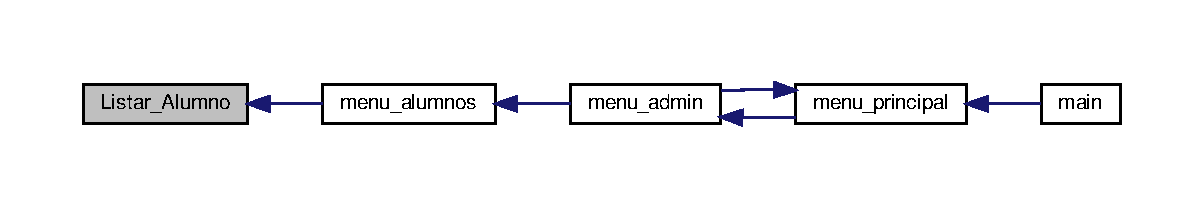
\includegraphics[width=350pt]{alumnos_8c_ac1b962c53e14b0375e64a44ebdcc38fa_icgraph}
\end{center}
\end{figure}
\mbox{\Hypertarget{alumnos_8c_a0ccfda8635c0219cd8397f0c76be0aa5}\label{alumnos_8c_a0ccfda8635c0219cd8397f0c76be0aa5}} 
\index{alumnos.\+c@{alumnos.\+c}!listar\+\_\+alumnos\+\_\+prof@{listar\+\_\+alumnos\+\_\+prof}}
\index{listar\+\_\+alumnos\+\_\+prof@{listar\+\_\+alumnos\+\_\+prof}!alumnos.\+c@{alumnos.\+c}}
\subsubsection{\texorpdfstring{listar\+\_\+alumnos\+\_\+prof()}{listar\_alumnos\_prof()}}
{\footnotesize\ttfamily char$\ast$ listar\+\_\+alumnos\+\_\+prof (\begin{DoxyParamCaption}\item[{\mbox{\hyperlink{structalumnos}{alumnos}} $\ast$}]{List\+\_\+\+Alumno,  }\item[{char $\ast$}]{id }\end{DoxyParamCaption})}

\mbox{\Hypertarget{alumnos_8c_a78832a2b6a02da48d43240f1ae7a273e}\label{alumnos_8c_a78832a2b6a02da48d43240f1ae7a273e}} 
\index{alumnos.\+c@{alumnos.\+c}!menu\+\_\+alumnos@{menu\+\_\+alumnos}}
\index{menu\+\_\+alumnos@{menu\+\_\+alumnos}!alumnos.\+c@{alumnos.\+c}}
\subsubsection{\texorpdfstring{menu\+\_\+alumnos()}{menu\_alumnos()}}
{\footnotesize\ttfamily void menu\+\_\+alumnos (\begin{DoxyParamCaption}\item[{\mbox{\hyperlink{structalumnos}{alumnos}} $\ast$}]{arr\+\_\+alumnos }\end{DoxyParamCaption})}

Here is the call graph for this function\+:\nopagebreak
\begin{figure}[H]
\begin{center}
\leavevmode
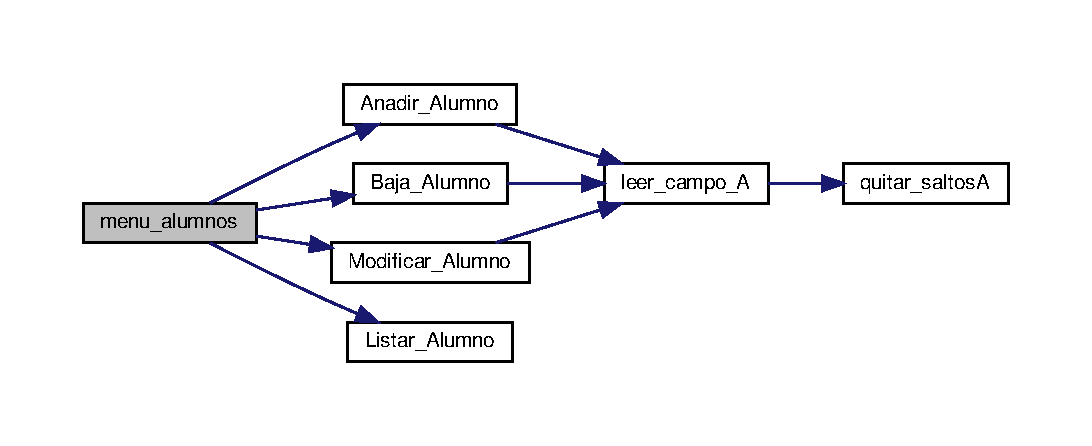
\includegraphics[width=350pt]{alumnos_8c_a78832a2b6a02da48d43240f1ae7a273e_cgraph}
\end{center}
\end{figure}
Here is the caller graph for this function\+:\nopagebreak
\begin{figure}[H]
\begin{center}
\leavevmode
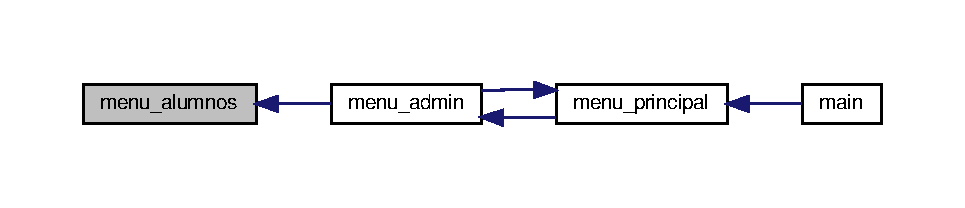
\includegraphics[width=350pt]{alumnos_8c_a78832a2b6a02da48d43240f1ae7a273e_icgraph}
\end{center}
\end{figure}
\mbox{\Hypertarget{alumnos_8c_a8dcb4e8881eb636706040c9e73d79ba4}\label{alumnos_8c_a8dcb4e8881eb636706040c9e73d79ba4}} 
\index{alumnos.\+c@{alumnos.\+c}!Modificar\+\_\+\+Alumno@{Modificar\+\_\+\+Alumno}}
\index{Modificar\+\_\+\+Alumno@{Modificar\+\_\+\+Alumno}!alumnos.\+c@{alumnos.\+c}}
\subsubsection{\texorpdfstring{Modificar\+\_\+\+Alumno()}{Modificar\_Alumno()}}
{\footnotesize\ttfamily void Modificar\+\_\+\+Alumno (\begin{DoxyParamCaption}\item[{\mbox{\hyperlink{structalumnos}{alumnos}} $\ast$}]{List\+\_\+\+Alumno }\end{DoxyParamCaption})}

Here is the call graph for this function\+:\nopagebreak
\begin{figure}[H]
\begin{center}
\leavevmode
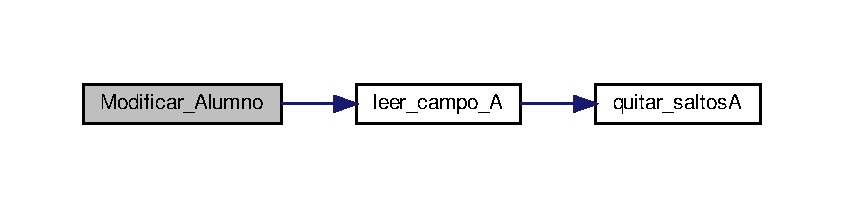
\includegraphics[width=350pt]{alumnos_8c_a8dcb4e8881eb636706040c9e73d79ba4_cgraph}
\end{center}
\end{figure}
Here is the caller graph for this function\+:\nopagebreak
\begin{figure}[H]
\begin{center}
\leavevmode
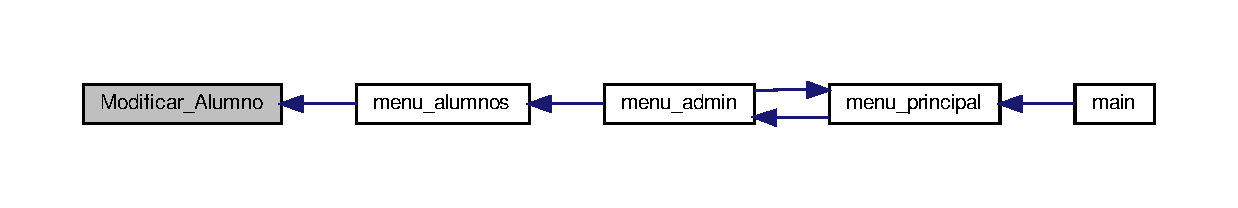
\includegraphics[width=350pt]{alumnos_8c_a8dcb4e8881eb636706040c9e73d79ba4_icgraph}
\end{center}
\end{figure}
\mbox{\Hypertarget{alumnos_8c_a23b200c89a3f9cd634292b6badc924bc}\label{alumnos_8c_a23b200c89a3f9cd634292b6badc924bc}} 
\index{alumnos.\+c@{alumnos.\+c}!Modificar\+\_\+\+Alumno\+\_\+ficha@{Modificar\+\_\+\+Alumno\+\_\+ficha}}
\index{Modificar\+\_\+\+Alumno\+\_\+ficha@{Modificar\+\_\+\+Alumno\+\_\+ficha}!alumnos.\+c@{alumnos.\+c}}
\subsubsection{\texorpdfstring{Modificar\+\_\+\+Alumno\+\_\+ficha()}{Modificar\_Alumno\_ficha()}}
{\footnotesize\ttfamily void Modificar\+\_\+\+Alumno\+\_\+ficha (\begin{DoxyParamCaption}\item[{\mbox{\hyperlink{structalumnos}{alumnos}} $\ast$}]{List\+\_\+\+Alumno,  }\item[{int}]{i }\end{DoxyParamCaption})}

Here is the call graph for this function\+:\nopagebreak
\begin{figure}[H]
\begin{center}
\leavevmode
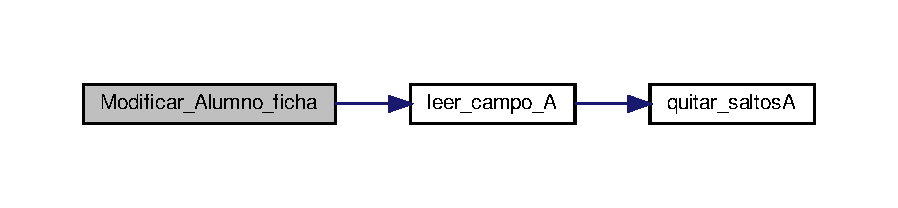
\includegraphics[width=350pt]{alumnos_8c_a23b200c89a3f9cd634292b6badc924bc_cgraph}
\end{center}
\end{figure}
Here is the caller graph for this function\+:\nopagebreak
\begin{figure}[H]
\begin{center}
\leavevmode
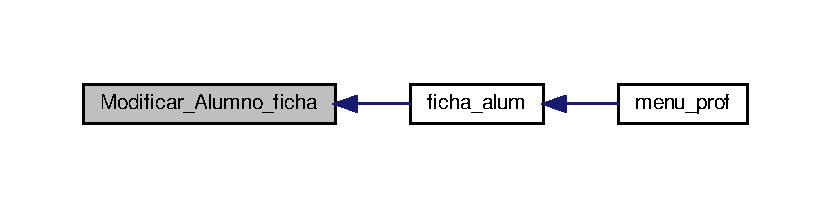
\includegraphics[width=350pt]{alumnos_8c_a23b200c89a3f9cd634292b6badc924bc_icgraph}
\end{center}
\end{figure}
\mbox{\Hypertarget{alumnos_8c_aa0ecdc5d299fcbde0eb715eb564f026f}\label{alumnos_8c_aa0ecdc5d299fcbde0eb715eb564f026f}} 
\index{alumnos.\+c@{alumnos.\+c}!quitar\+\_\+saltosA@{quitar\+\_\+saltosA}}
\index{quitar\+\_\+saltosA@{quitar\+\_\+saltosA}!alumnos.\+c@{alumnos.\+c}}
\subsubsection{\texorpdfstring{quitar\+\_\+saltos\+A()}{quitar\_saltosA()}}
{\footnotesize\ttfamily void quitar\+\_\+saltosA (\begin{DoxyParamCaption}\item[{char $\ast$}]{cadena }\end{DoxyParamCaption})}

Here is the caller graph for this function\+:\nopagebreak
\begin{figure}[H]
\begin{center}
\leavevmode
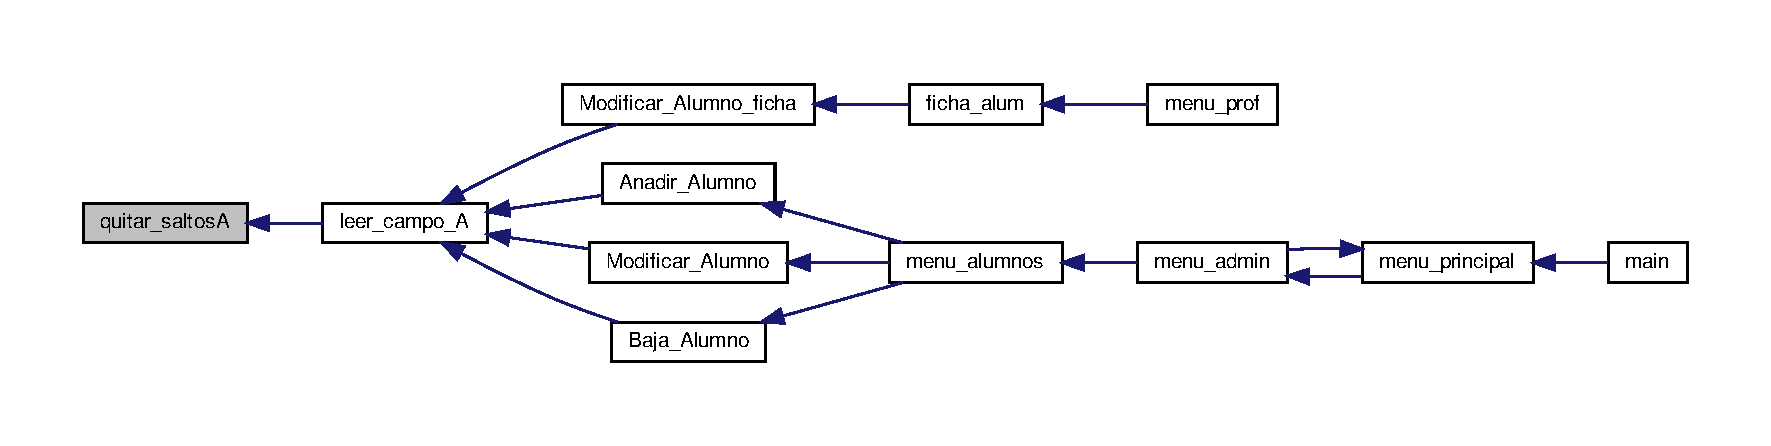
\includegraphics[width=350pt]{alumnos_8c_aa0ecdc5d299fcbde0eb715eb564f026f_icgraph}
\end{center}
\end{figure}


\subsection{Variable Documentation}
\mbox{\Hypertarget{alumnos_8c_a64e3b8d4f87de890cc5ee7edee65b616}\label{alumnos_8c_a64e3b8d4f87de890cc5ee7edee65b616}} 
\index{alumnos.\+c@{alumnos.\+c}!conta@{conta}}
\index{conta@{conta}!alumnos.\+c@{alumnos.\+c}}
\subsubsection{\texorpdfstring{conta}{conta}}
{\footnotesize\ttfamily int conta =0}


\hypertarget{alumnos_8h}{}\section{Referencia del Archivo alumnos.\+h}
\label{alumnos_8h}\index{alumnos.\+h@{alumnos.\+h}}
{\ttfamily \#include $<$stdlib.\+h$>$}\newline
{\ttfamily \#include $<$stdio.\+h$>$}\newline
Dependencia gráfica adjunta para alumnos.\+h\+:
\nopagebreak
\begin{figure}[H]
\begin{center}
\leavevmode
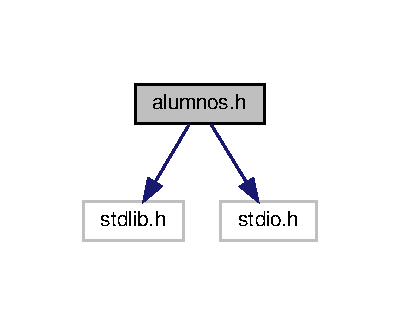
\includegraphics[width=192pt]{alumnos_8h__incl}
\end{center}
\end{figure}
Gráfico de los archivos que directa o indirectamente incluyen a este archivo\+:
\nopagebreak
\begin{figure}[H]
\begin{center}
\leavevmode
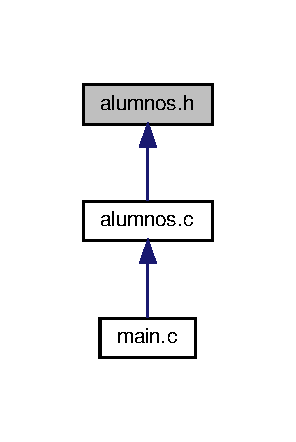
\includegraphics[width=142pt]{alumnos_8h__dep__incl}
\end{center}
\end{figure}
\subsection*{Funciones}
\begin{DoxyCompactItemize}
\item 
\mbox{\hyperlink{structalumnos}{alumnos}} $\ast$ \mbox{\hyperlink{alumnos_8h_acb60a266abe9b3631929cafc7077ee56}{Carga\+\_\+\+Alumno}} ()
\item 
void \mbox{\hyperlink{alumnos_8h_a7e65fac55eb382c0f8f45dc1c34b0dca}{Guardar\+\_\+\+Alumno}} (\mbox{\hyperlink{structalumnos}{alumnos}} $\ast$)
\item 
void \mbox{\hyperlink{alumnos_8h_a700183d8a00b761d4a6dc613a1526725}{Anadir\+\_\+\+Alumno}} (\mbox{\hyperlink{structalumnos}{alumnos}} $\ast$)
\item 
void \mbox{\hyperlink{alumnos_8h_aece0c54c25c5d6c034db5a2872d71ed7}{Listar\+\_\+\+Alumno}} (\mbox{\hyperlink{structalumnos}{alumnos}} $\ast$)
\item 
void \mbox{\hyperlink{alumnos_8h_a2ae61b7c43491e9e07855dde716f778c}{Modificar\+\_\+\+Alumno}} (\mbox{\hyperlink{structalumnos}{alumnos}} $\ast$)
\item 
void \mbox{\hyperlink{alumnos_8h_ac061cc5688bada3f4407aab402aad01c}{Baja\+\_\+\+Alumno}} (\mbox{\hyperlink{structalumnos}{alumnos}} $\ast$)
\item 
void \mbox{\hyperlink{alumnos_8h_a8dbfa0cb38f32ff6c1298094d2c67498}{menu\+\_\+alumnos}} ()
\item 
void \mbox{\hyperlink{alumnos_8h_a12f661aaa137adb1b3efc1cc516ee3fd}{ficha\+\_\+alum}} (\mbox{\hyperlink{structalumnos}{alumnos}} $\ast$, char $\ast$)
\item 
char $\ast$ \mbox{\hyperlink{alumnos_8h_ac5dc1be96545b748ecbd85064e56bfde}{listar\+\_\+alumnos\+\_\+prof}} (\mbox{\hyperlink{structalumnos}{alumnos}} $\ast$, char $\ast$)
\end{DoxyCompactItemize}


\subsection{Documentación de las funciones}
\mbox{\Hypertarget{alumnos_8h_a700183d8a00b761d4a6dc613a1526725}\label{alumnos_8h_a700183d8a00b761d4a6dc613a1526725}} 
\index{alumnos.\+h@{alumnos.\+h}!Anadir\+\_\+\+Alumno@{Anadir\+\_\+\+Alumno}}
\index{Anadir\+\_\+\+Alumno@{Anadir\+\_\+\+Alumno}!alumnos.\+h@{alumnos.\+h}}
\subsubsection{\texorpdfstring{Anadir\+\_\+\+Alumno()}{Anadir\_Alumno()}}
{\footnotesize\ttfamily void Anadir\+\_\+\+Alumno (\begin{DoxyParamCaption}\item[{\mbox{\hyperlink{structalumnos}{alumnos}} $\ast$}]{ }\end{DoxyParamCaption})}



Definición en la línea 146 del archivo alumnos.\+c.

Gráfico de llamadas para esta función\+:
\nopagebreak
\begin{figure}[H]
\begin{center}
\leavevmode
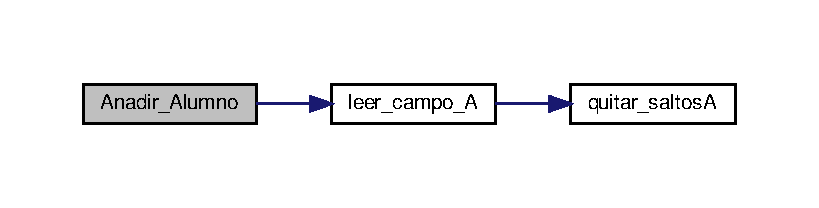
\includegraphics[width=350pt]{alumnos_8h_a700183d8a00b761d4a6dc613a1526725_cgraph}
\end{center}
\end{figure}
Gráfico de llamadas a esta función\+:
\nopagebreak
\begin{figure}[H]
\begin{center}
\leavevmode
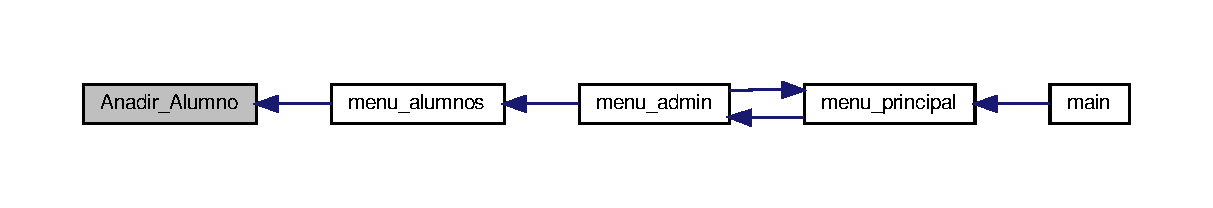
\includegraphics[width=350pt]{alumnos_8h_a700183d8a00b761d4a6dc613a1526725_icgraph}
\end{center}
\end{figure}
\mbox{\Hypertarget{alumnos_8h_ac061cc5688bada3f4407aab402aad01c}\label{alumnos_8h_ac061cc5688bada3f4407aab402aad01c}} 
\index{alumnos.\+h@{alumnos.\+h}!Baja\+\_\+\+Alumno@{Baja\+\_\+\+Alumno}}
\index{Baja\+\_\+\+Alumno@{Baja\+\_\+\+Alumno}!alumnos.\+h@{alumnos.\+h}}
\subsubsection{\texorpdfstring{Baja\+\_\+\+Alumno()}{Baja\_Alumno()}}
{\footnotesize\ttfamily void Baja\+\_\+\+Alumno (\begin{DoxyParamCaption}\item[{\mbox{\hyperlink{structalumnos}{alumnos}} $\ast$}]{ }\end{DoxyParamCaption})}



Definición en la línea 182 del archivo alumnos.\+c.

Gráfico de llamadas para esta función\+:
\nopagebreak
\begin{figure}[H]
\begin{center}
\leavevmode
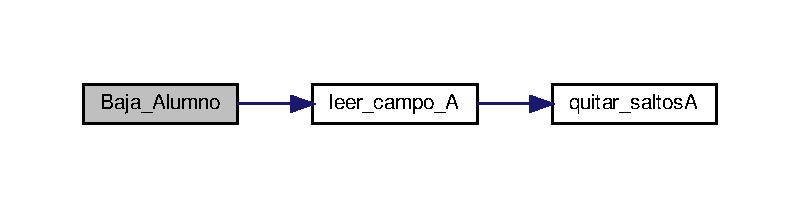
\includegraphics[width=350pt]{alumnos_8h_ac061cc5688bada3f4407aab402aad01c_cgraph}
\end{center}
\end{figure}
Gráfico de llamadas a esta función\+:
\nopagebreak
\begin{figure}[H]
\begin{center}
\leavevmode
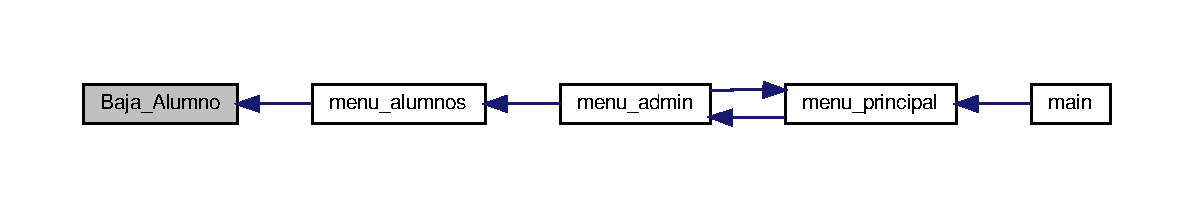
\includegraphics[width=350pt]{alumnos_8h_ac061cc5688bada3f4407aab402aad01c_icgraph}
\end{center}
\end{figure}
\mbox{\Hypertarget{alumnos_8h_acb60a266abe9b3631929cafc7077ee56}\label{alumnos_8h_acb60a266abe9b3631929cafc7077ee56}} 
\index{alumnos.\+h@{alumnos.\+h}!Carga\+\_\+\+Alumno@{Carga\+\_\+\+Alumno}}
\index{Carga\+\_\+\+Alumno@{Carga\+\_\+\+Alumno}!alumnos.\+h@{alumnos.\+h}}
\subsubsection{\texorpdfstring{Carga\+\_\+\+Alumno()}{Carga\_Alumno()}}
{\footnotesize\ttfamily \mbox{\hyperlink{structalumnos}{alumnos}}$\ast$ Carga\+\_\+\+Alumno (\begin{DoxyParamCaption}{ }\end{DoxyParamCaption})}



Definición en la línea 32 del archivo alumnos.\+c.

Gráfico de llamadas a esta función\+:
\nopagebreak
\begin{figure}[H]
\begin{center}
\leavevmode
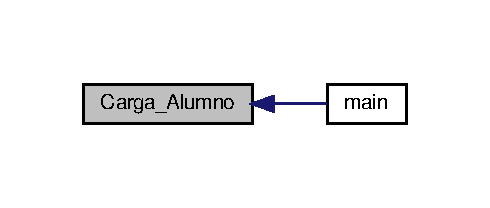
\includegraphics[width=235pt]{alumnos_8h_acb60a266abe9b3631929cafc7077ee56_icgraph}
\end{center}
\end{figure}
\mbox{\Hypertarget{alumnos_8h_a12f661aaa137adb1b3efc1cc516ee3fd}\label{alumnos_8h_a12f661aaa137adb1b3efc1cc516ee3fd}} 
\index{alumnos.\+h@{alumnos.\+h}!ficha\+\_\+alum@{ficha\+\_\+alum}}
\index{ficha\+\_\+alum@{ficha\+\_\+alum}!alumnos.\+h@{alumnos.\+h}}
\subsubsection{\texorpdfstring{ficha\+\_\+alum()}{ficha\_alum()}}
{\footnotesize\ttfamily void ficha\+\_\+alum (\begin{DoxyParamCaption}\item[{\mbox{\hyperlink{structalumnos}{alumnos}} $\ast$}]{,  }\item[{char $\ast$}]{ }\end{DoxyParamCaption})}



Definición en la línea 120 del archivo alumnos.\+c.

Gráfico de llamadas para esta función\+:
\nopagebreak
\begin{figure}[H]
\begin{center}
\leavevmode
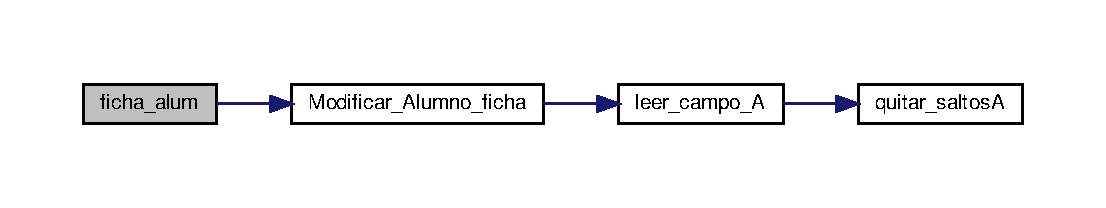
\includegraphics[width=350pt]{alumnos_8h_a12f661aaa137adb1b3efc1cc516ee3fd_cgraph}
\end{center}
\end{figure}
Gráfico de llamadas a esta función\+:
\nopagebreak
\begin{figure}[H]
\begin{center}
\leavevmode
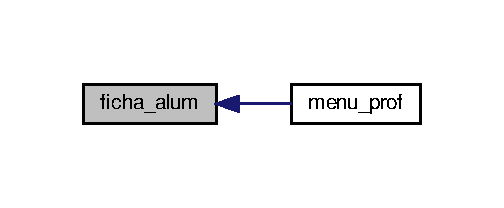
\includegraphics[width=242pt]{alumnos_8h_a12f661aaa137adb1b3efc1cc516ee3fd_icgraph}
\end{center}
\end{figure}
\mbox{\Hypertarget{alumnos_8h_a7e65fac55eb382c0f8f45dc1c34b0dca}\label{alumnos_8h_a7e65fac55eb382c0f8f45dc1c34b0dca}} 
\index{alumnos.\+h@{alumnos.\+h}!Guardar\+\_\+\+Alumno@{Guardar\+\_\+\+Alumno}}
\index{Guardar\+\_\+\+Alumno@{Guardar\+\_\+\+Alumno}!alumnos.\+h@{alumnos.\+h}}
\subsubsection{\texorpdfstring{Guardar\+\_\+\+Alumno()}{Guardar\_Alumno()}}
{\footnotesize\ttfamily void Guardar\+\_\+\+Alumno (\begin{DoxyParamCaption}\item[{\mbox{\hyperlink{structalumnos}{alumnos}} $\ast$}]{ }\end{DoxyParamCaption})}



Definición en la línea 215 del archivo alumnos.\+c.

Gráfico de llamadas a esta función\+:
\nopagebreak
\begin{figure}[H]
\begin{center}
\leavevmode
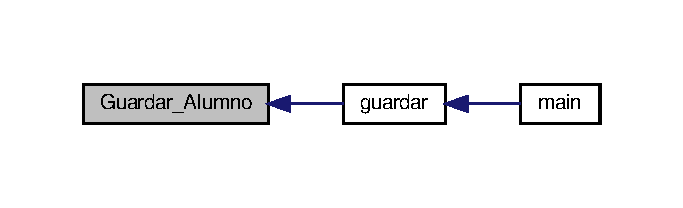
\includegraphics[width=328pt]{alumnos_8h_a7e65fac55eb382c0f8f45dc1c34b0dca_icgraph}
\end{center}
\end{figure}
\mbox{\Hypertarget{alumnos_8h_aece0c54c25c5d6c034db5a2872d71ed7}\label{alumnos_8h_aece0c54c25c5d6c034db5a2872d71ed7}} 
\index{alumnos.\+h@{alumnos.\+h}!Listar\+\_\+\+Alumno@{Listar\+\_\+\+Alumno}}
\index{Listar\+\_\+\+Alumno@{Listar\+\_\+\+Alumno}!alumnos.\+h@{alumnos.\+h}}
\subsubsection{\texorpdfstring{Listar\+\_\+\+Alumno()}{Listar\_Alumno()}}
{\footnotesize\ttfamily void Listar\+\_\+\+Alumno (\begin{DoxyParamCaption}\item[{\mbox{\hyperlink{structalumnos}{alumnos}} $\ast$}]{ }\end{DoxyParamCaption})}



Definición en la línea 157 del archivo alumnos.\+c.

Gráfico de llamadas a esta función\+:
\nopagebreak
\begin{figure}[H]
\begin{center}
\leavevmode
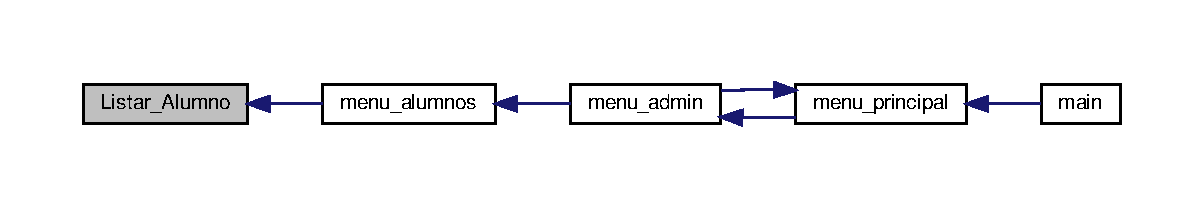
\includegraphics[width=350pt]{alumnos_8h_aece0c54c25c5d6c034db5a2872d71ed7_icgraph}
\end{center}
\end{figure}
\mbox{\Hypertarget{alumnos_8h_ac5dc1be96545b748ecbd85064e56bfde}\label{alumnos_8h_ac5dc1be96545b748ecbd85064e56bfde}} 
\index{alumnos.\+h@{alumnos.\+h}!listar\+\_\+alumnos\+\_\+prof@{listar\+\_\+alumnos\+\_\+prof}}
\index{listar\+\_\+alumnos\+\_\+prof@{listar\+\_\+alumnos\+\_\+prof}!alumnos.\+h@{alumnos.\+h}}
\subsubsection{\texorpdfstring{listar\+\_\+alumnos\+\_\+prof()}{listar\_alumnos\_prof()}}
{\footnotesize\ttfamily char$\ast$ listar\+\_\+alumnos\+\_\+prof (\begin{DoxyParamCaption}\item[{\mbox{\hyperlink{structalumnos}{alumnos}} $\ast$}]{,  }\item[{char $\ast$}]{ }\end{DoxyParamCaption})}



Definición en la línea 113 del archivo alumnos.\+c.

\mbox{\Hypertarget{alumnos_8h_a8dbfa0cb38f32ff6c1298094d2c67498}\label{alumnos_8h_a8dbfa0cb38f32ff6c1298094d2c67498}} 
\index{alumnos.\+h@{alumnos.\+h}!menu\+\_\+alumnos@{menu\+\_\+alumnos}}
\index{menu\+\_\+alumnos@{menu\+\_\+alumnos}!alumnos.\+h@{alumnos.\+h}}
\subsubsection{\texorpdfstring{menu\+\_\+alumnos()}{menu\_alumnos()}}
{\footnotesize\ttfamily void menu\+\_\+alumnos (\begin{DoxyParamCaption}{ }\end{DoxyParamCaption})}

\mbox{\Hypertarget{alumnos_8h_a2ae61b7c43491e9e07855dde716f778c}\label{alumnos_8h_a2ae61b7c43491e9e07855dde716f778c}} 
\index{alumnos.\+h@{alumnos.\+h}!Modificar\+\_\+\+Alumno@{Modificar\+\_\+\+Alumno}}
\index{Modificar\+\_\+\+Alumno@{Modificar\+\_\+\+Alumno}!alumnos.\+h@{alumnos.\+h}}
\subsubsection{\texorpdfstring{Modificar\+\_\+\+Alumno()}{Modificar\_Alumno()}}
{\footnotesize\ttfamily void Modificar\+\_\+\+Alumno (\begin{DoxyParamCaption}\item[{\mbox{\hyperlink{structalumnos}{alumnos}} $\ast$}]{ }\end{DoxyParamCaption})}



Definición en la línea 163 del archivo alumnos.\+c.

Gráfico de llamadas para esta función\+:
\nopagebreak
\begin{figure}[H]
\begin{center}
\leavevmode
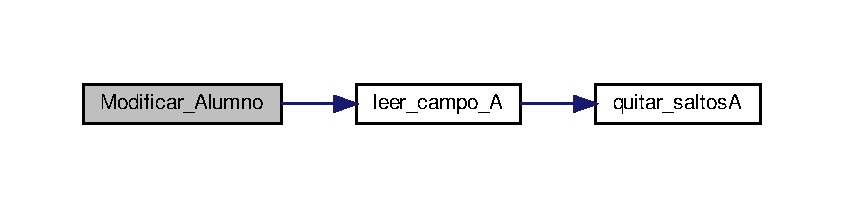
\includegraphics[width=350pt]{alumnos_8h_a2ae61b7c43491e9e07855dde716f778c_cgraph}
\end{center}
\end{figure}
Gráfico de llamadas a esta función\+:
\nopagebreak
\begin{figure}[H]
\begin{center}
\leavevmode
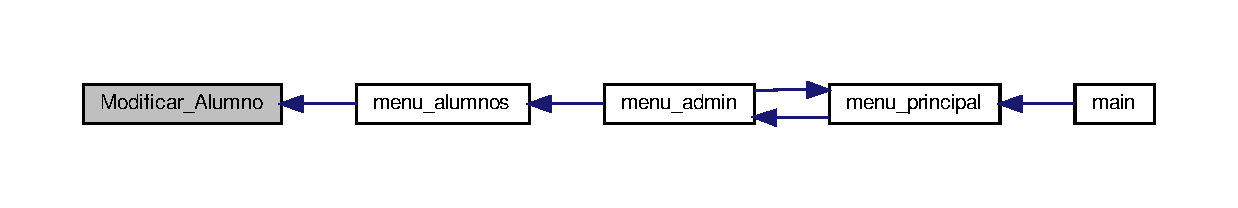
\includegraphics[width=350pt]{alumnos_8h_a2ae61b7c43491e9e07855dde716f778c_icgraph}
\end{center}
\end{figure}

\hypertarget{auxiliar_8c}{}\section{auxiliar.\+c File Reference}
\label{auxiliar_8c}\index{auxiliar.\+c@{auxiliar.\+c}}
{\ttfamily \#include $<$stdio.\+h$>$}\newline
{\ttfamily \#include $<$stdlib.\+h$>$}\newline
{\ttfamily \#include $<$string.\+h$>$}\newline
{\ttfamily \#include \char`\"{}auxiliar.\+h\char`\"{}}\newline
Include dependency graph for auxiliar.\+c\+:\nopagebreak
\begin{figure}[H]
\begin{center}
\leavevmode
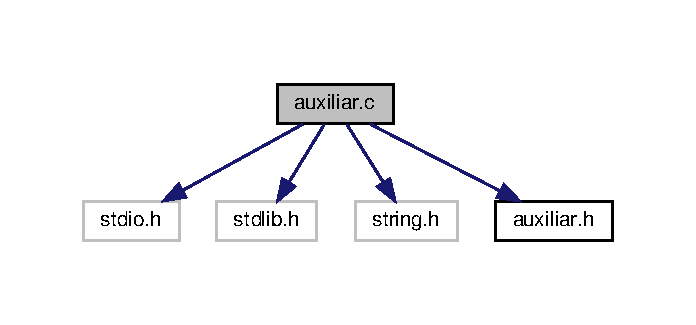
\includegraphics[width=334pt]{auxiliar_8c__incl}
\end{center}
\end{figure}
This graph shows which files directly or indirectly include this file\+:\nopagebreak
\begin{figure}[H]
\begin{center}
\leavevmode
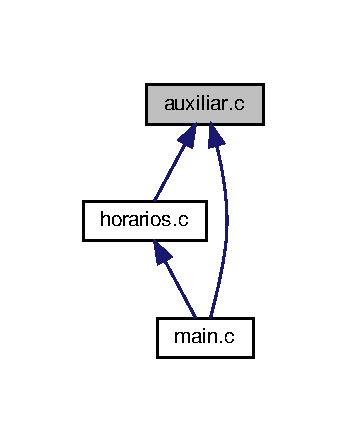
\includegraphics[width=167pt]{auxiliar_8c__dep__incl}
\end{center}
\end{figure}
\subsection*{Functions}
\begin{DoxyCompactItemize}
\item 
int \mbox{\hyperlink{auxiliar_8c_a32079d110eb0a5afff6f9e6a7b04068f}{get\+\_\+line}} (char $\ast$prmpt, char $\ast$buff, size\+\_\+t sz)
\item 
void \mbox{\hyperlink{auxiliar_8c_a7504a2d2a4e24f9454e81228c76ab706}{convertir\+\_\+digito\+\_\+cadena}} (char $\ast$target, char $\ast$longitud\+\_\+cadena, int numero)
\item 
void \mbox{\hyperlink{auxiliar_8c_a81c76a28dc198558e047094b3b54e446}{str\+\_\+replace}} (char $\ast$target, const char $\ast$needle, const char $\ast$replacement)
\item 
int \mbox{\hyperlink{auxiliar_8c_af563356e908679d2838195c29ffaa5b3}{fecha\+\_\+correcta}} (char $\ast$fecha)
\item 
int \mbox{\hyperlink{auxiliar_8c_aa0b5b35c3b50e4f533a31f5e98cd4a1a}{cuenta\+\_\+lineas}} (char $\ast$nombre\+\_\+fichero)
\item 
char $\ast$ \mbox{\hyperlink{auxiliar_8c_abdbe3a8a14ee84bfc7d3f33a4a327979}{leer\+\_\+campo\+\_\+m}} (int largo)
\end{DoxyCompactItemize}


\subsection{Function Documentation}
\mbox{\Hypertarget{auxiliar_8c_a7504a2d2a4e24f9454e81228c76ab706}\label{auxiliar_8c_a7504a2d2a4e24f9454e81228c76ab706}} 
\index{auxiliar.\+c@{auxiliar.\+c}!convertir\+\_\+digito\+\_\+cadena@{convertir\+\_\+digito\+\_\+cadena}}
\index{convertir\+\_\+digito\+\_\+cadena@{convertir\+\_\+digito\+\_\+cadena}!auxiliar.\+c@{auxiliar.\+c}}
\subsubsection{\texorpdfstring{convertir\+\_\+digito\+\_\+cadena()}{convertir\_digito\_cadena()}}
{\footnotesize\ttfamily void convertir\+\_\+digito\+\_\+cadena (\begin{DoxyParamCaption}\item[{char $\ast$}]{target,  }\item[{char $\ast$}]{longitud\+\_\+cadena,  }\item[{int}]{numero }\end{DoxyParamCaption})}

\mbox{\Hypertarget{auxiliar_8c_aa0b5b35c3b50e4f533a31f5e98cd4a1a}\label{auxiliar_8c_aa0b5b35c3b50e4f533a31f5e98cd4a1a}} 
\index{auxiliar.\+c@{auxiliar.\+c}!cuenta\+\_\+lineas@{cuenta\+\_\+lineas}}
\index{cuenta\+\_\+lineas@{cuenta\+\_\+lineas}!auxiliar.\+c@{auxiliar.\+c}}
\subsubsection{\texorpdfstring{cuenta\+\_\+lineas()}{cuenta\_lineas()}}
{\footnotesize\ttfamily int cuenta\+\_\+lineas (\begin{DoxyParamCaption}\item[{char $\ast$}]{nombre\+\_\+fichero }\end{DoxyParamCaption})}

Here is the caller graph for this function\+:\nopagebreak
\begin{figure}[H]
\begin{center}
\leavevmode
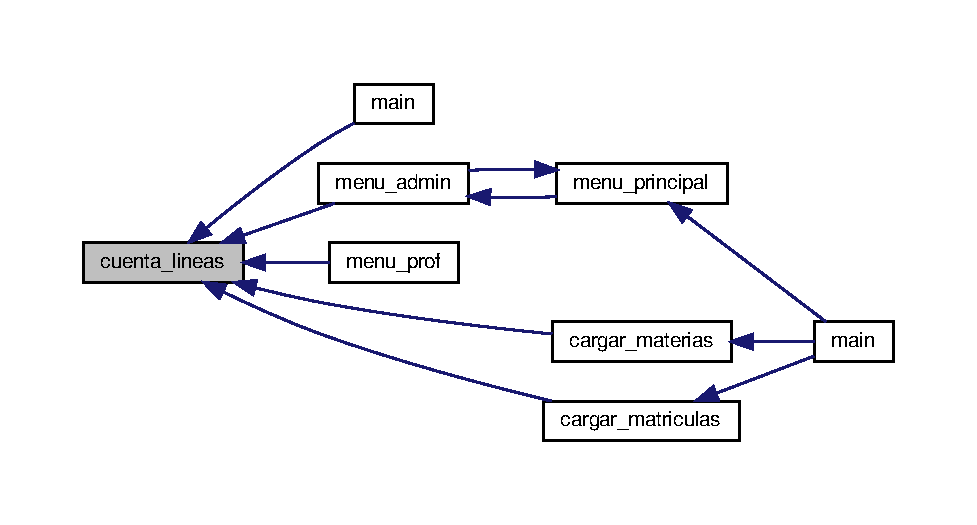
\includegraphics[width=350pt]{auxiliar_8c_aa0b5b35c3b50e4f533a31f5e98cd4a1a_icgraph}
\end{center}
\end{figure}
\mbox{\Hypertarget{auxiliar_8c_af563356e908679d2838195c29ffaa5b3}\label{auxiliar_8c_af563356e908679d2838195c29ffaa5b3}} 
\index{auxiliar.\+c@{auxiliar.\+c}!fecha\+\_\+correcta@{fecha\+\_\+correcta}}
\index{fecha\+\_\+correcta@{fecha\+\_\+correcta}!auxiliar.\+c@{auxiliar.\+c}}
\subsubsection{\texorpdfstring{fecha\+\_\+correcta()}{fecha\_correcta()}}
{\footnotesize\ttfamily int fecha\+\_\+correcta (\begin{DoxyParamCaption}\item[{char $\ast$}]{fecha }\end{DoxyParamCaption})}

Here is the caller graph for this function\+:\nopagebreak
\begin{figure}[H]
\begin{center}
\leavevmode
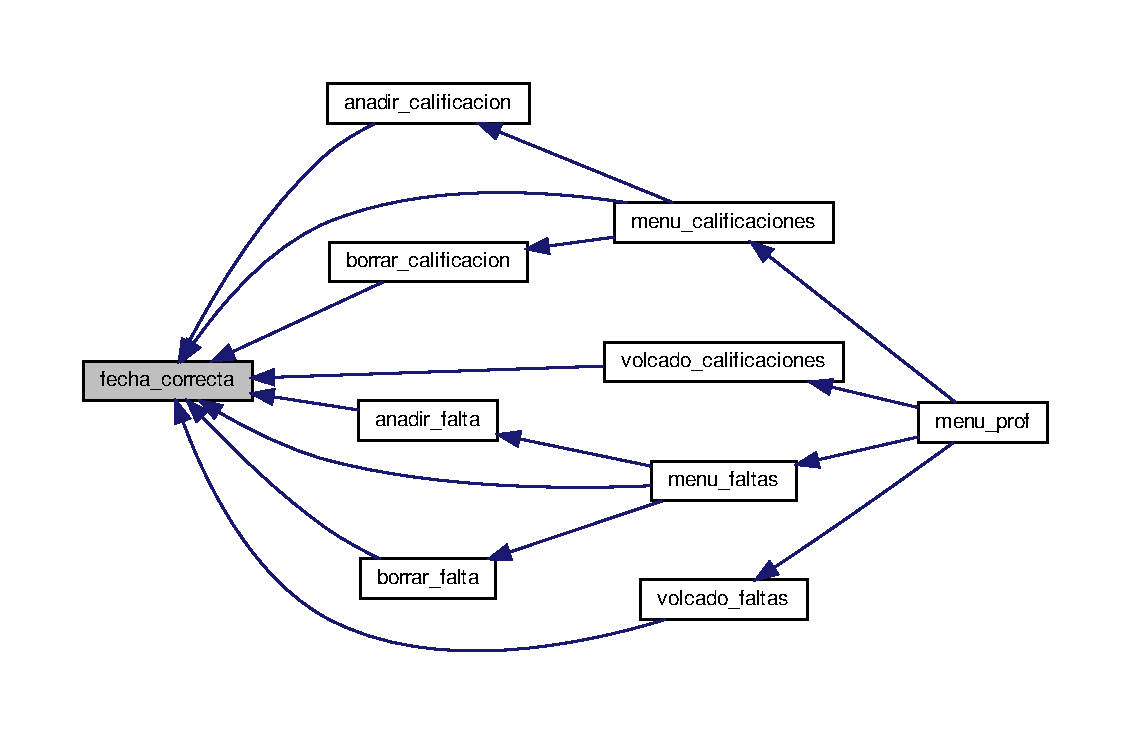
\includegraphics[width=350pt]{auxiliar_8c_af563356e908679d2838195c29ffaa5b3_icgraph}
\end{center}
\end{figure}
\mbox{\Hypertarget{auxiliar_8c_a32079d110eb0a5afff6f9e6a7b04068f}\label{auxiliar_8c_a32079d110eb0a5afff6f9e6a7b04068f}} 
\index{auxiliar.\+c@{auxiliar.\+c}!get\+\_\+line@{get\+\_\+line}}
\index{get\+\_\+line@{get\+\_\+line}!auxiliar.\+c@{auxiliar.\+c}}
\subsubsection{\texorpdfstring{get\+\_\+line()}{get\_line()}}
{\footnotesize\ttfamily int get\+\_\+line (\begin{DoxyParamCaption}\item[{char $\ast$}]{prmpt,  }\item[{char $\ast$}]{buff,  }\item[{size\+\_\+t}]{sz }\end{DoxyParamCaption})}

Here is the caller graph for this function\+:\nopagebreak
\begin{figure}[H]
\begin{center}
\leavevmode
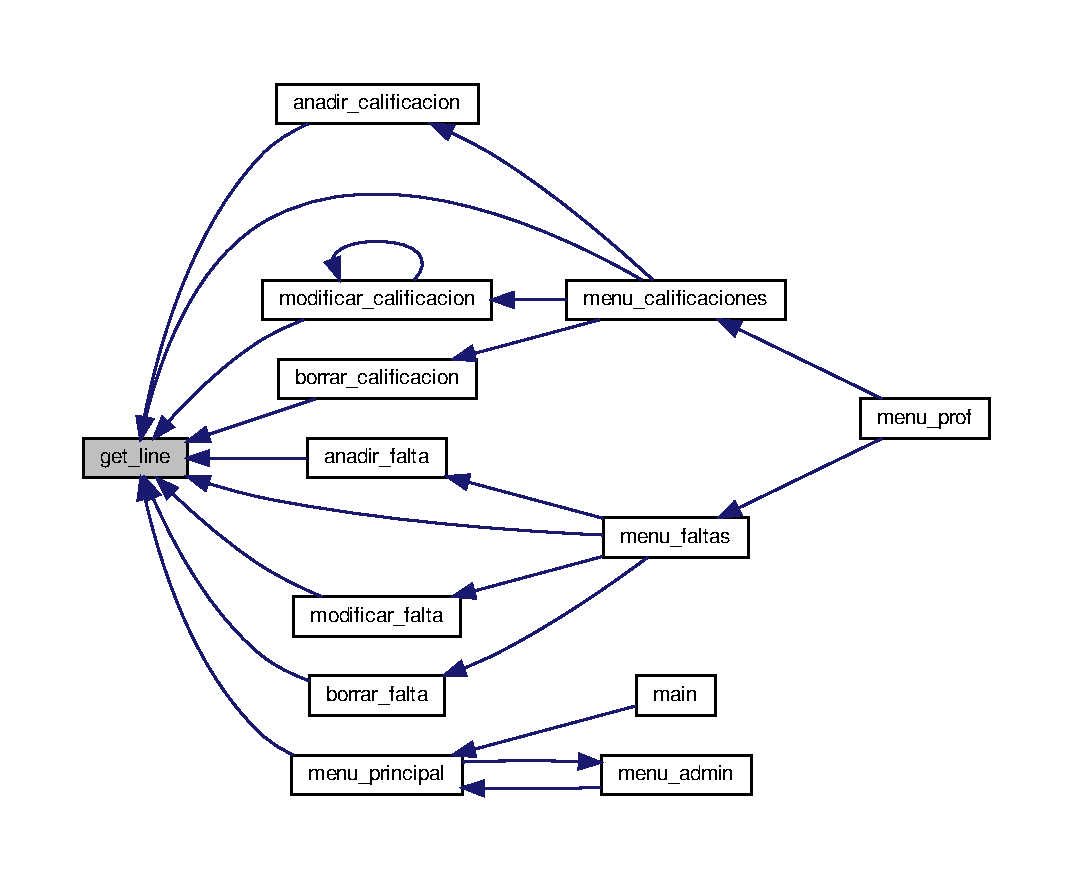
\includegraphics[width=350pt]{auxiliar_8c_a32079d110eb0a5afff6f9e6a7b04068f_icgraph}
\end{center}
\end{figure}
\mbox{\Hypertarget{auxiliar_8c_abdbe3a8a14ee84bfc7d3f33a4a327979}\label{auxiliar_8c_abdbe3a8a14ee84bfc7d3f33a4a327979}} 
\index{auxiliar.\+c@{auxiliar.\+c}!leer\+\_\+campo\+\_\+m@{leer\+\_\+campo\+\_\+m}}
\index{leer\+\_\+campo\+\_\+m@{leer\+\_\+campo\+\_\+m}!auxiliar.\+c@{auxiliar.\+c}}
\subsubsection{\texorpdfstring{leer\+\_\+campo\+\_\+m()}{leer\_campo\_m()}}
{\footnotesize\ttfamily char$\ast$ leer\+\_\+campo\+\_\+m (\begin{DoxyParamCaption}\item[{int}]{largo }\end{DoxyParamCaption})}

Here is the caller graph for this function\+:\nopagebreak
\begin{figure}[H]
\begin{center}
\leavevmode
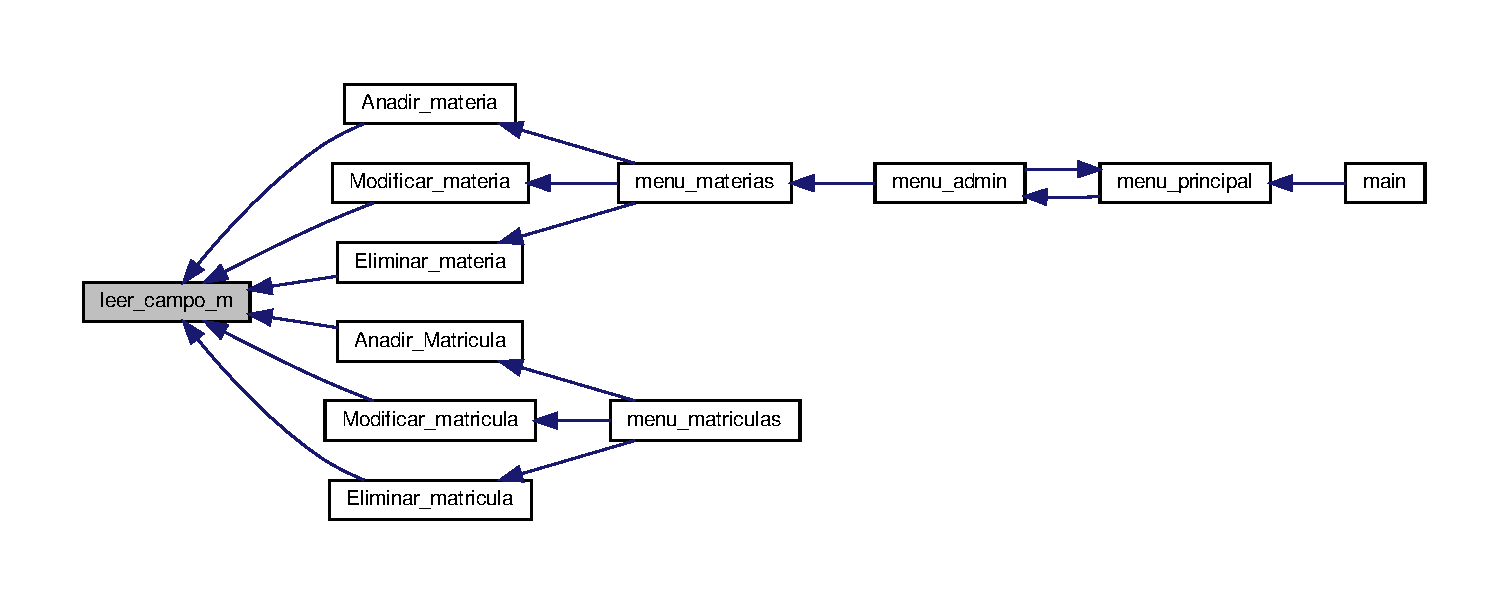
\includegraphics[width=350pt]{auxiliar_8c_abdbe3a8a14ee84bfc7d3f33a4a327979_icgraph}
\end{center}
\end{figure}
\mbox{\Hypertarget{auxiliar_8c_a81c76a28dc198558e047094b3b54e446}\label{auxiliar_8c_a81c76a28dc198558e047094b3b54e446}} 
\index{auxiliar.\+c@{auxiliar.\+c}!str\+\_\+replace@{str\+\_\+replace}}
\index{str\+\_\+replace@{str\+\_\+replace}!auxiliar.\+c@{auxiliar.\+c}}
\subsubsection{\texorpdfstring{str\+\_\+replace()}{str\_replace()}}
{\footnotesize\ttfamily void str\+\_\+replace (\begin{DoxyParamCaption}\item[{char $\ast$}]{target,  }\item[{const char $\ast$}]{needle,  }\item[{const char $\ast$}]{replacement }\end{DoxyParamCaption})}

Here is the caller graph for this function\+:\nopagebreak
\begin{figure}[H]
\begin{center}
\leavevmode
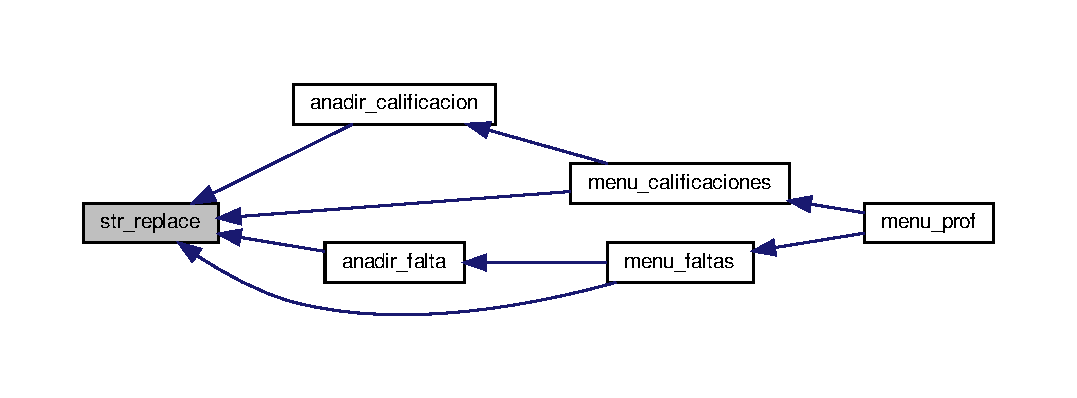
\includegraphics[width=350pt]{auxiliar_8c_a81c76a28dc198558e047094b3b54e446_icgraph}
\end{center}
\end{figure}

\hypertarget{auxiliar_8h}{}\section{auxiliar.\+h File Reference}
\label{auxiliar_8h}\index{auxiliar.\+h@{auxiliar.\+h}}
This graph shows which files directly or indirectly include this file\+:\nopagebreak
\begin{figure}[H]
\begin{center}
\leavevmode
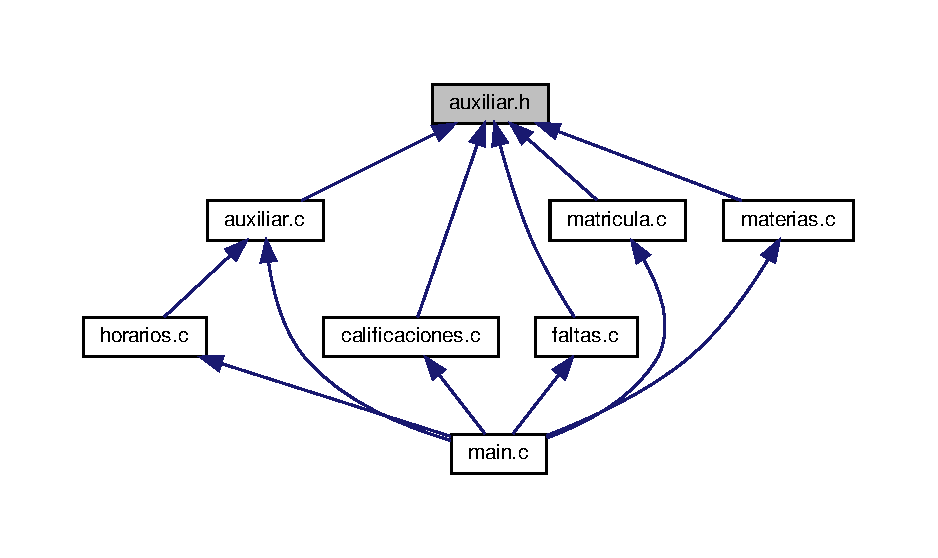
\includegraphics[width=350pt]{auxiliar_8h__dep__incl}
\end{center}
\end{figure}
\subsection*{Macros}
\begin{DoxyCompactItemize}
\item 
\#define \mbox{\hyperlink{auxiliar_8h_a34995b955465f6bbb37c359173d50477}{A\+N\+S\+I\+\_\+\+C\+O\+L\+O\+R\+\_\+\+R\+ED}}~\char`\"{}\textbackslash{}x1b\mbox{[}31m\char`\"{}
\item 
\#define \mbox{\hyperlink{auxiliar_8h_a966c72d8d733c7734c6c784753d894c7}{A\+N\+S\+I\+\_\+\+C\+O\+L\+O\+R\+\_\+\+G\+R\+E\+EN}}~\char`\"{}\textbackslash{}x1b\mbox{[}32m\char`\"{}
\item 
\#define \mbox{\hyperlink{auxiliar_8h_a5a123b382640b3aa65dd5db386002fbc}{A\+N\+S\+I\+\_\+\+C\+O\+L\+O\+R\+\_\+\+Y\+E\+L\+L\+OW}}~\char`\"{}\textbackslash{}x1b\mbox{[}33m\char`\"{}
\item 
\#define \mbox{\hyperlink{auxiliar_8h_aca16e6a49eb51333c5fd3eee19487315}{A\+N\+S\+I\+\_\+\+C\+O\+L\+O\+R\+\_\+\+B\+L\+UE}}~\char`\"{}\textbackslash{}x1b\mbox{[}34m\char`\"{}
\item 
\#define \mbox{\hyperlink{auxiliar_8h_acb30614ba1535da5b9d0c490b3c10515}{A\+N\+S\+I\+\_\+\+C\+O\+L\+O\+R\+\_\+\+M\+A\+G\+E\+N\+TA}}~\char`\"{}\textbackslash{}x1b\mbox{[}35m\char`\"{}
\item 
\#define \mbox{\hyperlink{auxiliar_8h_a8d0b0043e152438bb39b918a1f98c65f}{A\+N\+S\+I\+\_\+\+C\+O\+L\+O\+R\+\_\+\+C\+Y\+AN}}~\char`\"{}\textbackslash{}x1b\mbox{[}36m\char`\"{}
\item 
\#define \mbox{\hyperlink{auxiliar_8h_a92a364c2b863dde1a024a77eac2a5b3b}{A\+N\+S\+I\+\_\+\+C\+O\+L\+O\+R\+\_\+\+R\+E\+S\+ET}}~\char`\"{}\textbackslash{}x1b\mbox{[}0m\char`\"{}
\item 
\#define \mbox{\hyperlink{auxiliar_8h_aba51915c87d64af47fb1cc59348961c9}{OK}}~0
\item 
\#define \mbox{\hyperlink{auxiliar_8h_ad62650a8615e3aa9191d667f58c439f0}{N\+O\+\_\+\+I\+N\+P\+UT}}~1
\item 
\#define \mbox{\hyperlink{auxiliar_8h_a3ee622568eda5bfdd3a6dbd3c34048de}{T\+O\+O\+\_\+\+L\+O\+NG}}~2
\end{DoxyCompactItemize}
\subsection*{Functions}
\begin{DoxyCompactItemize}
\item 
int \mbox{\hyperlink{auxiliar_8h_aa0b5b35c3b50e4f533a31f5e98cd4a1a}{cuenta\+\_\+lineas}} (char $\ast$nombre\+\_\+fichero)
\item 
int \mbox{\hyperlink{auxiliar_8h_af563356e908679d2838195c29ffaa5b3}{fecha\+\_\+correcta}} (char $\ast$fecha)
\item 
void \mbox{\hyperlink{auxiliar_8h_a81c76a28dc198558e047094b3b54e446}{str\+\_\+replace}} (char $\ast$target, const char $\ast$needle, const char $\ast$replacement)
\item 
void \mbox{\hyperlink{auxiliar_8h_a7504a2d2a4e24f9454e81228c76ab706}{convertir\+\_\+digito\+\_\+cadena}} (char $\ast$target, char $\ast$longitud\+\_\+cadena, int numero)
\item 
int \mbox{\hyperlink{auxiliar_8h_a32079d110eb0a5afff6f9e6a7b04068f}{get\+\_\+line}} (char $\ast$prmpt, char $\ast$buff, size\+\_\+t sz)
\item 
char $\ast$ \mbox{\hyperlink{auxiliar_8h_abdbe3a8a14ee84bfc7d3f33a4a327979}{leer\+\_\+campo\+\_\+m}} (int largo)
\end{DoxyCompactItemize}


\subsection{Macro Definition Documentation}
\mbox{\Hypertarget{auxiliar_8h_aca16e6a49eb51333c5fd3eee19487315}\label{auxiliar_8h_aca16e6a49eb51333c5fd3eee19487315}} 
\index{auxiliar.\+h@{auxiliar.\+h}!A\+N\+S\+I\+\_\+\+C\+O\+L\+O\+R\+\_\+\+B\+L\+UE@{A\+N\+S\+I\+\_\+\+C\+O\+L\+O\+R\+\_\+\+B\+L\+UE}}
\index{A\+N\+S\+I\+\_\+\+C\+O\+L\+O\+R\+\_\+\+B\+L\+UE@{A\+N\+S\+I\+\_\+\+C\+O\+L\+O\+R\+\_\+\+B\+L\+UE}!auxiliar.\+h@{auxiliar.\+h}}
\subsubsection{\texorpdfstring{A\+N\+S\+I\+\_\+\+C\+O\+L\+O\+R\+\_\+\+B\+L\+UE}{ANSI\_COLOR\_BLUE}}
{\footnotesize\ttfamily \#define A\+N\+S\+I\+\_\+\+C\+O\+L\+O\+R\+\_\+\+B\+L\+UE~\char`\"{}\textbackslash{}x1b\mbox{[}34m\char`\"{}}

\mbox{\Hypertarget{auxiliar_8h_a8d0b0043e152438bb39b918a1f98c65f}\label{auxiliar_8h_a8d0b0043e152438bb39b918a1f98c65f}} 
\index{auxiliar.\+h@{auxiliar.\+h}!A\+N\+S\+I\+\_\+\+C\+O\+L\+O\+R\+\_\+\+C\+Y\+AN@{A\+N\+S\+I\+\_\+\+C\+O\+L\+O\+R\+\_\+\+C\+Y\+AN}}
\index{A\+N\+S\+I\+\_\+\+C\+O\+L\+O\+R\+\_\+\+C\+Y\+AN@{A\+N\+S\+I\+\_\+\+C\+O\+L\+O\+R\+\_\+\+C\+Y\+AN}!auxiliar.\+h@{auxiliar.\+h}}
\subsubsection{\texorpdfstring{A\+N\+S\+I\+\_\+\+C\+O\+L\+O\+R\+\_\+\+C\+Y\+AN}{ANSI\_COLOR\_CYAN}}
{\footnotesize\ttfamily \#define A\+N\+S\+I\+\_\+\+C\+O\+L\+O\+R\+\_\+\+C\+Y\+AN~\char`\"{}\textbackslash{}x1b\mbox{[}36m\char`\"{}}

\mbox{\Hypertarget{auxiliar_8h_a966c72d8d733c7734c6c784753d894c7}\label{auxiliar_8h_a966c72d8d733c7734c6c784753d894c7}} 
\index{auxiliar.\+h@{auxiliar.\+h}!A\+N\+S\+I\+\_\+\+C\+O\+L\+O\+R\+\_\+\+G\+R\+E\+EN@{A\+N\+S\+I\+\_\+\+C\+O\+L\+O\+R\+\_\+\+G\+R\+E\+EN}}
\index{A\+N\+S\+I\+\_\+\+C\+O\+L\+O\+R\+\_\+\+G\+R\+E\+EN@{A\+N\+S\+I\+\_\+\+C\+O\+L\+O\+R\+\_\+\+G\+R\+E\+EN}!auxiliar.\+h@{auxiliar.\+h}}
\subsubsection{\texorpdfstring{A\+N\+S\+I\+\_\+\+C\+O\+L\+O\+R\+\_\+\+G\+R\+E\+EN}{ANSI\_COLOR\_GREEN}}
{\footnotesize\ttfamily \#define A\+N\+S\+I\+\_\+\+C\+O\+L\+O\+R\+\_\+\+G\+R\+E\+EN~\char`\"{}\textbackslash{}x1b\mbox{[}32m\char`\"{}}

\mbox{\Hypertarget{auxiliar_8h_acb30614ba1535da5b9d0c490b3c10515}\label{auxiliar_8h_acb30614ba1535da5b9d0c490b3c10515}} 
\index{auxiliar.\+h@{auxiliar.\+h}!A\+N\+S\+I\+\_\+\+C\+O\+L\+O\+R\+\_\+\+M\+A\+G\+E\+N\+TA@{A\+N\+S\+I\+\_\+\+C\+O\+L\+O\+R\+\_\+\+M\+A\+G\+E\+N\+TA}}
\index{A\+N\+S\+I\+\_\+\+C\+O\+L\+O\+R\+\_\+\+M\+A\+G\+E\+N\+TA@{A\+N\+S\+I\+\_\+\+C\+O\+L\+O\+R\+\_\+\+M\+A\+G\+E\+N\+TA}!auxiliar.\+h@{auxiliar.\+h}}
\subsubsection{\texorpdfstring{A\+N\+S\+I\+\_\+\+C\+O\+L\+O\+R\+\_\+\+M\+A\+G\+E\+N\+TA}{ANSI\_COLOR\_MAGENTA}}
{\footnotesize\ttfamily \#define A\+N\+S\+I\+\_\+\+C\+O\+L\+O\+R\+\_\+\+M\+A\+G\+E\+N\+TA~\char`\"{}\textbackslash{}x1b\mbox{[}35m\char`\"{}}

\mbox{\Hypertarget{auxiliar_8h_a34995b955465f6bbb37c359173d50477}\label{auxiliar_8h_a34995b955465f6bbb37c359173d50477}} 
\index{auxiliar.\+h@{auxiliar.\+h}!A\+N\+S\+I\+\_\+\+C\+O\+L\+O\+R\+\_\+\+R\+ED@{A\+N\+S\+I\+\_\+\+C\+O\+L\+O\+R\+\_\+\+R\+ED}}
\index{A\+N\+S\+I\+\_\+\+C\+O\+L\+O\+R\+\_\+\+R\+ED@{A\+N\+S\+I\+\_\+\+C\+O\+L\+O\+R\+\_\+\+R\+ED}!auxiliar.\+h@{auxiliar.\+h}}
\subsubsection{\texorpdfstring{A\+N\+S\+I\+\_\+\+C\+O\+L\+O\+R\+\_\+\+R\+ED}{ANSI\_COLOR\_RED}}
{\footnotesize\ttfamily \#define A\+N\+S\+I\+\_\+\+C\+O\+L\+O\+R\+\_\+\+R\+ED~\char`\"{}\textbackslash{}x1b\mbox{[}31m\char`\"{}}

\mbox{\Hypertarget{auxiliar_8h_a92a364c2b863dde1a024a77eac2a5b3b}\label{auxiliar_8h_a92a364c2b863dde1a024a77eac2a5b3b}} 
\index{auxiliar.\+h@{auxiliar.\+h}!A\+N\+S\+I\+\_\+\+C\+O\+L\+O\+R\+\_\+\+R\+E\+S\+ET@{A\+N\+S\+I\+\_\+\+C\+O\+L\+O\+R\+\_\+\+R\+E\+S\+ET}}
\index{A\+N\+S\+I\+\_\+\+C\+O\+L\+O\+R\+\_\+\+R\+E\+S\+ET@{A\+N\+S\+I\+\_\+\+C\+O\+L\+O\+R\+\_\+\+R\+E\+S\+ET}!auxiliar.\+h@{auxiliar.\+h}}
\subsubsection{\texorpdfstring{A\+N\+S\+I\+\_\+\+C\+O\+L\+O\+R\+\_\+\+R\+E\+S\+ET}{ANSI\_COLOR\_RESET}}
{\footnotesize\ttfamily \#define A\+N\+S\+I\+\_\+\+C\+O\+L\+O\+R\+\_\+\+R\+E\+S\+ET~\char`\"{}\textbackslash{}x1b\mbox{[}0m\char`\"{}}

\mbox{\Hypertarget{auxiliar_8h_a5a123b382640b3aa65dd5db386002fbc}\label{auxiliar_8h_a5a123b382640b3aa65dd5db386002fbc}} 
\index{auxiliar.\+h@{auxiliar.\+h}!A\+N\+S\+I\+\_\+\+C\+O\+L\+O\+R\+\_\+\+Y\+E\+L\+L\+OW@{A\+N\+S\+I\+\_\+\+C\+O\+L\+O\+R\+\_\+\+Y\+E\+L\+L\+OW}}
\index{A\+N\+S\+I\+\_\+\+C\+O\+L\+O\+R\+\_\+\+Y\+E\+L\+L\+OW@{A\+N\+S\+I\+\_\+\+C\+O\+L\+O\+R\+\_\+\+Y\+E\+L\+L\+OW}!auxiliar.\+h@{auxiliar.\+h}}
\subsubsection{\texorpdfstring{A\+N\+S\+I\+\_\+\+C\+O\+L\+O\+R\+\_\+\+Y\+E\+L\+L\+OW}{ANSI\_COLOR\_YELLOW}}
{\footnotesize\ttfamily \#define A\+N\+S\+I\+\_\+\+C\+O\+L\+O\+R\+\_\+\+Y\+E\+L\+L\+OW~\char`\"{}\textbackslash{}x1b\mbox{[}33m\char`\"{}}

\mbox{\Hypertarget{auxiliar_8h_ad62650a8615e3aa9191d667f58c439f0}\label{auxiliar_8h_ad62650a8615e3aa9191d667f58c439f0}} 
\index{auxiliar.\+h@{auxiliar.\+h}!N\+O\+\_\+\+I\+N\+P\+UT@{N\+O\+\_\+\+I\+N\+P\+UT}}
\index{N\+O\+\_\+\+I\+N\+P\+UT@{N\+O\+\_\+\+I\+N\+P\+UT}!auxiliar.\+h@{auxiliar.\+h}}
\subsubsection{\texorpdfstring{N\+O\+\_\+\+I\+N\+P\+UT}{NO\_INPUT}}
{\footnotesize\ttfamily \#define N\+O\+\_\+\+I\+N\+P\+UT~1}

\mbox{\Hypertarget{auxiliar_8h_aba51915c87d64af47fb1cc59348961c9}\label{auxiliar_8h_aba51915c87d64af47fb1cc59348961c9}} 
\index{auxiliar.\+h@{auxiliar.\+h}!OK@{OK}}
\index{OK@{OK}!auxiliar.\+h@{auxiliar.\+h}}
\subsubsection{\texorpdfstring{OK}{OK}}
{\footnotesize\ttfamily \#define OK~0}

\mbox{\Hypertarget{auxiliar_8h_a3ee622568eda5bfdd3a6dbd3c34048de}\label{auxiliar_8h_a3ee622568eda5bfdd3a6dbd3c34048de}} 
\index{auxiliar.\+h@{auxiliar.\+h}!T\+O\+O\+\_\+\+L\+O\+NG@{T\+O\+O\+\_\+\+L\+O\+NG}}
\index{T\+O\+O\+\_\+\+L\+O\+NG@{T\+O\+O\+\_\+\+L\+O\+NG}!auxiliar.\+h@{auxiliar.\+h}}
\subsubsection{\texorpdfstring{T\+O\+O\+\_\+\+L\+O\+NG}{TOO\_LONG}}
{\footnotesize\ttfamily \#define T\+O\+O\+\_\+\+L\+O\+NG~2}



\subsection{Function Documentation}
\mbox{\Hypertarget{auxiliar_8h_a7504a2d2a4e24f9454e81228c76ab706}\label{auxiliar_8h_a7504a2d2a4e24f9454e81228c76ab706}} 
\index{auxiliar.\+h@{auxiliar.\+h}!convertir\+\_\+digito\+\_\+cadena@{convertir\+\_\+digito\+\_\+cadena}}
\index{convertir\+\_\+digito\+\_\+cadena@{convertir\+\_\+digito\+\_\+cadena}!auxiliar.\+h@{auxiliar.\+h}}
\subsubsection{\texorpdfstring{convertir\+\_\+digito\+\_\+cadena()}{convertir\_digito\_cadena()}}
{\footnotesize\ttfamily void convertir\+\_\+digito\+\_\+cadena (\begin{DoxyParamCaption}\item[{char $\ast$}]{target,  }\item[{char $\ast$}]{longitud\+\_\+cadena,  }\item[{int}]{numero }\end{DoxyParamCaption})}

\mbox{\Hypertarget{auxiliar_8h_aa0b5b35c3b50e4f533a31f5e98cd4a1a}\label{auxiliar_8h_aa0b5b35c3b50e4f533a31f5e98cd4a1a}} 
\index{auxiliar.\+h@{auxiliar.\+h}!cuenta\+\_\+lineas@{cuenta\+\_\+lineas}}
\index{cuenta\+\_\+lineas@{cuenta\+\_\+lineas}!auxiliar.\+h@{auxiliar.\+h}}
\subsubsection{\texorpdfstring{cuenta\+\_\+lineas()}{cuenta\_lineas()}}
{\footnotesize\ttfamily int cuenta\+\_\+lineas (\begin{DoxyParamCaption}\item[{char $\ast$}]{nombre\+\_\+fichero }\end{DoxyParamCaption})}

Here is the caller graph for this function\+:\nopagebreak
\begin{figure}[H]
\begin{center}
\leavevmode
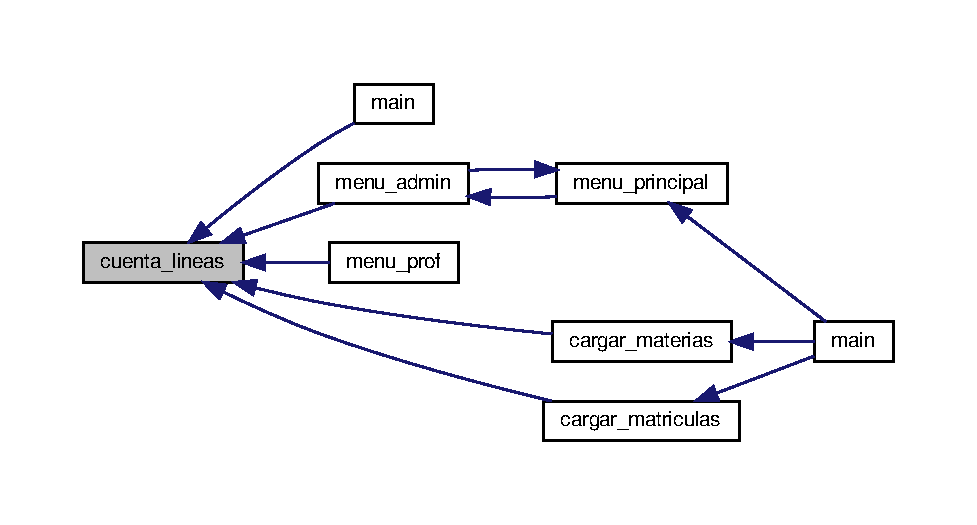
\includegraphics[width=350pt]{auxiliar_8h_aa0b5b35c3b50e4f533a31f5e98cd4a1a_icgraph}
\end{center}
\end{figure}
\mbox{\Hypertarget{auxiliar_8h_af563356e908679d2838195c29ffaa5b3}\label{auxiliar_8h_af563356e908679d2838195c29ffaa5b3}} 
\index{auxiliar.\+h@{auxiliar.\+h}!fecha\+\_\+correcta@{fecha\+\_\+correcta}}
\index{fecha\+\_\+correcta@{fecha\+\_\+correcta}!auxiliar.\+h@{auxiliar.\+h}}
\subsubsection{\texorpdfstring{fecha\+\_\+correcta()}{fecha\_correcta()}}
{\footnotesize\ttfamily int fecha\+\_\+correcta (\begin{DoxyParamCaption}\item[{char $\ast$}]{fecha }\end{DoxyParamCaption})}

Here is the caller graph for this function\+:\nopagebreak
\begin{figure}[H]
\begin{center}
\leavevmode
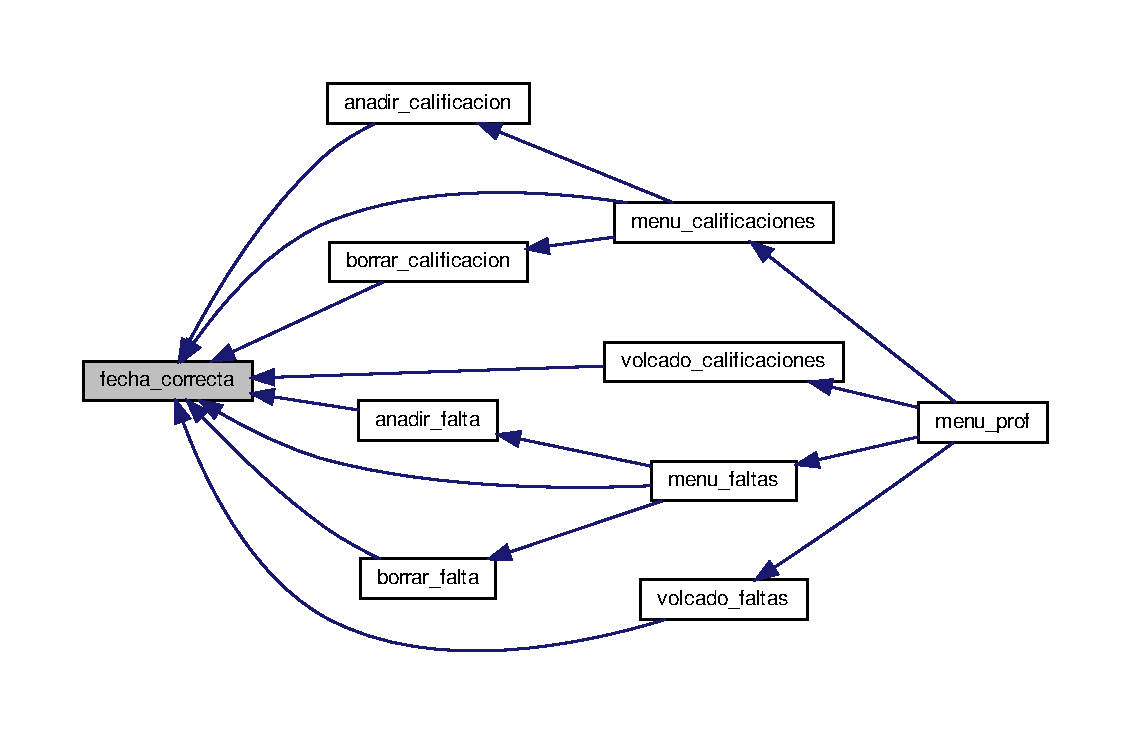
\includegraphics[width=350pt]{auxiliar_8h_af563356e908679d2838195c29ffaa5b3_icgraph}
\end{center}
\end{figure}
\mbox{\Hypertarget{auxiliar_8h_a32079d110eb0a5afff6f9e6a7b04068f}\label{auxiliar_8h_a32079d110eb0a5afff6f9e6a7b04068f}} 
\index{auxiliar.\+h@{auxiliar.\+h}!get\+\_\+line@{get\+\_\+line}}
\index{get\+\_\+line@{get\+\_\+line}!auxiliar.\+h@{auxiliar.\+h}}
\subsubsection{\texorpdfstring{get\+\_\+line()}{get\_line()}}
{\footnotesize\ttfamily int get\+\_\+line (\begin{DoxyParamCaption}\item[{char $\ast$}]{prmpt,  }\item[{char $\ast$}]{buff,  }\item[{size\+\_\+t}]{sz }\end{DoxyParamCaption})}

Here is the caller graph for this function\+:\nopagebreak
\begin{figure}[H]
\begin{center}
\leavevmode
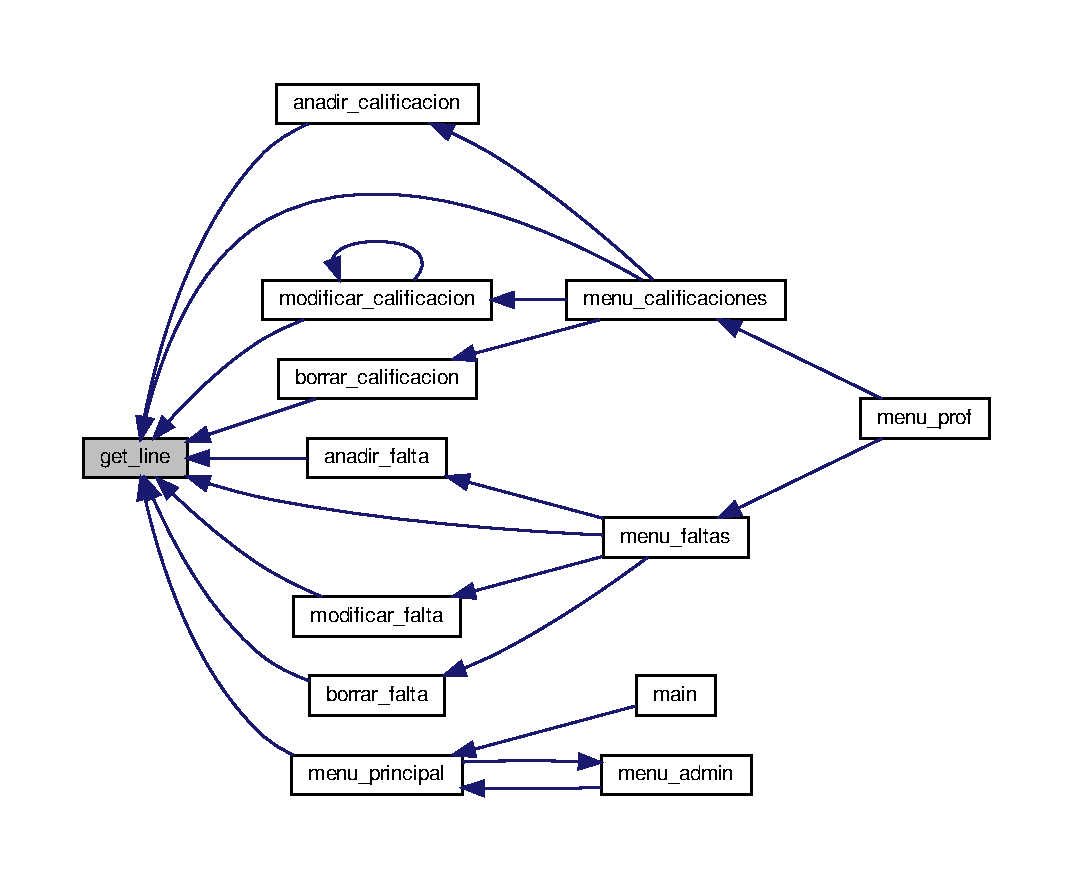
\includegraphics[width=350pt]{auxiliar_8h_a32079d110eb0a5afff6f9e6a7b04068f_icgraph}
\end{center}
\end{figure}
\mbox{\Hypertarget{auxiliar_8h_abdbe3a8a14ee84bfc7d3f33a4a327979}\label{auxiliar_8h_abdbe3a8a14ee84bfc7d3f33a4a327979}} 
\index{auxiliar.\+h@{auxiliar.\+h}!leer\+\_\+campo\+\_\+m@{leer\+\_\+campo\+\_\+m}}
\index{leer\+\_\+campo\+\_\+m@{leer\+\_\+campo\+\_\+m}!auxiliar.\+h@{auxiliar.\+h}}
\subsubsection{\texorpdfstring{leer\+\_\+campo\+\_\+m()}{leer\_campo\_m()}}
{\footnotesize\ttfamily char$\ast$ leer\+\_\+campo\+\_\+m (\begin{DoxyParamCaption}\item[{int}]{largo }\end{DoxyParamCaption})}

Here is the caller graph for this function\+:\nopagebreak
\begin{figure}[H]
\begin{center}
\leavevmode
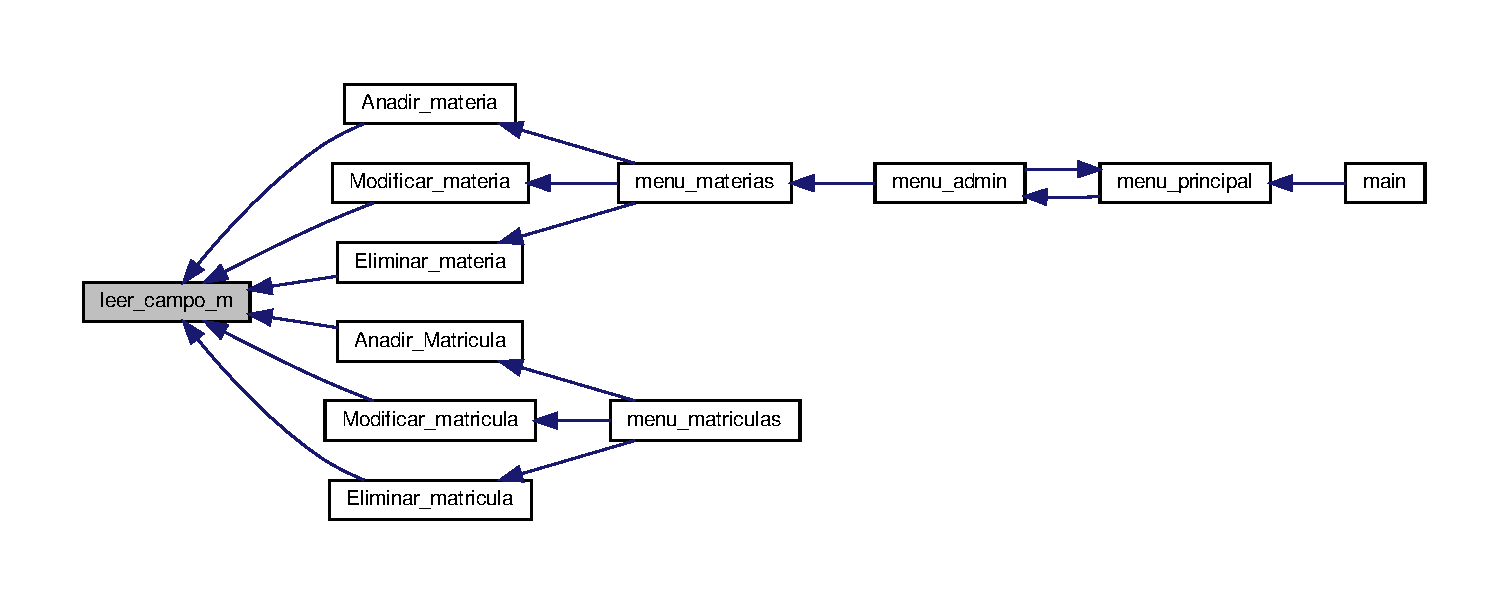
\includegraphics[width=350pt]{auxiliar_8h_abdbe3a8a14ee84bfc7d3f33a4a327979_icgraph}
\end{center}
\end{figure}
\mbox{\Hypertarget{auxiliar_8h_a81c76a28dc198558e047094b3b54e446}\label{auxiliar_8h_a81c76a28dc198558e047094b3b54e446}} 
\index{auxiliar.\+h@{auxiliar.\+h}!str\+\_\+replace@{str\+\_\+replace}}
\index{str\+\_\+replace@{str\+\_\+replace}!auxiliar.\+h@{auxiliar.\+h}}
\subsubsection{\texorpdfstring{str\+\_\+replace()}{str\_replace()}}
{\footnotesize\ttfamily void str\+\_\+replace (\begin{DoxyParamCaption}\item[{char $\ast$}]{target,  }\item[{const char $\ast$}]{needle,  }\item[{const char $\ast$}]{replacement }\end{DoxyParamCaption})}

Here is the caller graph for this function\+:\nopagebreak
\begin{figure}[H]
\begin{center}
\leavevmode
\includegraphics[width=350pt]{auxiliar_8h_a81c76a28dc198558e047094b3b54e446_icgraph}
\end{center}
\end{figure}

\hypertarget{calificaciones_8c}{}\section{calificaciones.\+c File Reference}
\label{calificaciones_8c}\index{calificaciones.\+c@{calificaciones.\+c}}
{\ttfamily \#include $<$stdio.\+h$>$}\newline
{\ttfamily \#include $<$stdlib.\+h$>$}\newline
{\ttfamily \#include $<$string.\+h$>$}\newline
{\ttfamily \#include \char`\"{}estructuras.\+h\char`\"{}}\newline
{\ttfamily \#include \char`\"{}auxiliar.\+h\char`\"{}}\newline
{\ttfamily \#include \char`\"{}calificaciones.\+h\char`\"{}}\newline
Include dependency graph for calificaciones.\+c\+:\nopagebreak
\begin{figure}[H]
\begin{center}
\leavevmode
\includegraphics[width=350pt]{calificaciones_8c__incl}
\end{center}
\end{figure}
This graph shows which files directly or indirectly include this file\+:\nopagebreak
\begin{figure}[H]
\begin{center}
\leavevmode
\includegraphics[width=164pt]{calificaciones_8c__dep__incl}
\end{center}
\end{figure}
\subsection*{Macros}
\begin{DoxyCompactItemize}
\item 
\#define \mbox{\hyperlink{calificaciones_8c_a5e7b25d6d6af977a017f9c93795ddb42}{M\+S\+G\+\_\+\+E\+R\+R\+O\+R\+\_\+\+N\+O\+TA}}~\char`\"{}No se admite como nota un valor inferior a 0 o superior a 10. Vuelva a intentarlo.\char`\"{}
\end{DoxyCompactItemize}
\subsection*{Functions}
\begin{DoxyCompactItemize}
\item 
int \mbox{\hyperlink{calificaciones_8c_aea947664e70772081dfa8ca1c52deb8d}{get\+\_\+longitud\+\_\+array\+\_\+calificaciones}} ()
\item 
int \mbox{\hyperlink{calificaciones_8c_a9483b8ffdfbb64b41447e365a3beb949}{nota\+\_\+valida}} (int nota, char $\ast$msg\+\_\+error)
\item 
void \mbox{\hyperlink{calificaciones_8c_a8499c1b281ab61f888cc659c3ea4a467}{buscar\+\_\+por\+\_\+materia}} (\mbox{\hyperlink{structcalificaciones}{calificaciones}} $\ast$list\+\_\+calificaciones, int id\+\_\+materia, \mbox{\hyperlink{structcalificaciones}{calificaciones}} $\ast$new\+\_\+list\+\_\+calificaciones, int longitud\+\_\+array)
\item 
void \mbox{\hyperlink{calificaciones_8c_a42463725127809cf3a21e41cab0a3b87}{buscar\+\_\+por\+\_\+alumno}} (\mbox{\hyperlink{structcalificaciones}{calificaciones}} $\ast$list\+\_\+calificaciones, int id\+\_\+alumno, \mbox{\hyperlink{structcalificaciones}{calificaciones}} $\ast$new\+\_\+list\+\_\+calificaciones, int longitud\+\_\+array)
\item 
void \mbox{\hyperlink{calificaciones_8c_a21abc134b66a3519979b8874b1d5973f}{print\+\_\+calificaciones\+\_\+por\+\_\+materia}} (\mbox{\hyperlink{structcalificaciones}{calificaciones}} $\ast$list\+\_\+calificaciones, int id\+\_\+materia, int longitud\+\_\+array)
\item 
void \mbox{\hyperlink{calificaciones_8c_ac715ee6871bcf139f60f3e3856f9d52f}{print\+\_\+calificaciones\+\_\+por\+\_\+alumno}} (\mbox{\hyperlink{structcalificaciones}{calificaciones}} $\ast$list\+\_\+calificaciones, int id\+\_\+alumno, int longitud\+\_\+array)
\item 
void \mbox{\hyperlink{calificaciones_8c_a2cec64ccdfe397e356898dc36c38c113}{print\+\_\+calificaciones\+\_\+criba}} (\mbox{\hyperlink{structcalificaciones}{calificaciones}} $\ast$list\+\_\+calificaciones, int $\ast$array\+\_\+datos, int longitud\+\_\+array)
\item 
\mbox{\hyperlink{structcalificaciones}{calificaciones}} $\ast$ \mbox{\hyperlink{calificaciones_8c_acca13e62fda4252c798b061adbf1c3b7}{anadir\+\_\+calificacion}} (\mbox{\hyperlink{structcalificaciones}{calificaciones}} $\ast$$\ast$list\+\_\+calificaciones, char datos\mbox{[}$\,$\mbox{]}\mbox{[}100\mbox{]}, int $\ast$longitud\+\_\+array)
\item 
void \mbox{\hyperlink{calificaciones_8c_a02a7c0ebe5e1312deb40cc4e481f82b6}{modificar\+\_\+calificacion}} (\mbox{\hyperlink{structcalificaciones}{calificaciones}} $\ast$list\+\_\+calificaciones, char datos\mbox{[}$\,$\mbox{]}\mbox{[}100\mbox{]}, int longitud\+\_\+array)
\item 
\mbox{\hyperlink{structcalificaciones}{calificaciones}} $\ast$ \mbox{\hyperlink{calificaciones_8c_a881cebfd4a7e933bbf2f4b878b11f0aa}{borrar\+\_\+calificacion}} (\mbox{\hyperlink{structcalificaciones}{calificaciones}} $\ast$$\ast$list\+\_\+calificaciones, char datos\mbox{[}$\,$\mbox{]}\mbox{[}100\mbox{]}, int $\ast$longitud\+\_\+array)
\item 
\mbox{\hyperlink{structcalificaciones}{calificaciones}} $\ast$ \mbox{\hyperlink{calificaciones_8c_abc9de671fc1b7b0ce38c34c72df7cbb3}{menu\+\_\+calificaciones}} (\mbox{\hyperlink{structcalificaciones}{calificaciones}} $\ast$list\+\_\+calificaciones, int $\ast$array\+\_\+datos, int longitud\+\_\+array)
\item 
void \mbox{\hyperlink{calificaciones_8c_a8252b1da04b93917487275be8a584210}{volcado\+\_\+calificaciones}} (F\+I\+LE $\ast$f, \mbox{\hyperlink{structcalificaciones}{calificaciones}} $\ast$list\+\_\+calificaciones, char $\ast$nom\+\_\+file, int longitud\+\_\+array)
\item 
void \mbox{\hyperlink{calificaciones_8c_a1392a5533577ef7383e5a9aeafe4dad4}{cargar\+\_\+calificaciones}} (F\+I\+LE $\ast$f, \mbox{\hyperlink{structcalificaciones}{calificaciones}} $\ast$list\+\_\+calificaciones)
\end{DoxyCompactItemize}
\subsection*{Variables}
\begin{DoxyCompactItemize}
\item 
int \mbox{\hyperlink{calificaciones_8c_aa7c327e827ac42d133740dd1a4ffbc33}{L\+O\+N\+G\+I\+T\+U\+D\+\_\+\+A\+R\+R\+A\+Y\+\_\+\+C\+A\+L\+I\+F\+I\+C\+A\+C\+I\+O\+N\+ES}}
\end{DoxyCompactItemize}


\subsection{Macro Definition Documentation}
\mbox{\Hypertarget{calificaciones_8c_a5e7b25d6d6af977a017f9c93795ddb42}\label{calificaciones_8c_a5e7b25d6d6af977a017f9c93795ddb42}} 
\index{calificaciones.\+c@{calificaciones.\+c}!M\+S\+G\+\_\+\+E\+R\+R\+O\+R\+\_\+\+N\+O\+TA@{M\+S\+G\+\_\+\+E\+R\+R\+O\+R\+\_\+\+N\+O\+TA}}
\index{M\+S\+G\+\_\+\+E\+R\+R\+O\+R\+\_\+\+N\+O\+TA@{M\+S\+G\+\_\+\+E\+R\+R\+O\+R\+\_\+\+N\+O\+TA}!calificaciones.\+c@{calificaciones.\+c}}
\subsubsection{\texorpdfstring{M\+S\+G\+\_\+\+E\+R\+R\+O\+R\+\_\+\+N\+O\+TA}{MSG\_ERROR\_NOTA}}
{\footnotesize\ttfamily \#define M\+S\+G\+\_\+\+E\+R\+R\+O\+R\+\_\+\+N\+O\+TA~\char`\"{}No se admite como nota un valor inferior a 0 o superior a 10. Vuelva a intentarlo.\char`\"{}}



\subsection{Function Documentation}
\mbox{\Hypertarget{calificaciones_8c_acca13e62fda4252c798b061adbf1c3b7}\label{calificaciones_8c_acca13e62fda4252c798b061adbf1c3b7}} 
\index{calificaciones.\+c@{calificaciones.\+c}!anadir\+\_\+calificacion@{anadir\+\_\+calificacion}}
\index{anadir\+\_\+calificacion@{anadir\+\_\+calificacion}!calificaciones.\+c@{calificaciones.\+c}}
\subsubsection{\texorpdfstring{anadir\+\_\+calificacion()}{anadir\_calificacion()}}
{\footnotesize\ttfamily \mbox{\hyperlink{structcalificaciones}{calificaciones}}$\ast$ anadir\+\_\+calificacion (\begin{DoxyParamCaption}\item[{\mbox{\hyperlink{structcalificaciones}{calificaciones}} $\ast$$\ast$}]{list\+\_\+calificaciones,  }\item[{char}]{datos\mbox{[}$\,$\mbox{]}\mbox{[}100\mbox{]},  }\item[{int $\ast$}]{longitud\+\_\+array }\end{DoxyParamCaption})}

Here is the call graph for this function\+:\nopagebreak
\begin{figure}[H]
\begin{center}
\leavevmode
\includegraphics[width=294pt]{calificaciones_8c_acca13e62fda4252c798b061adbf1c3b7_cgraph}
\end{center}
\end{figure}
Here is the caller graph for this function\+:\nopagebreak
\begin{figure}[H]
\begin{center}
\leavevmode
\includegraphics[width=350pt]{calificaciones_8c_acca13e62fda4252c798b061adbf1c3b7_icgraph}
\end{center}
\end{figure}
\mbox{\Hypertarget{calificaciones_8c_a881cebfd4a7e933bbf2f4b878b11f0aa}\label{calificaciones_8c_a881cebfd4a7e933bbf2f4b878b11f0aa}} 
\index{calificaciones.\+c@{calificaciones.\+c}!borrar\+\_\+calificacion@{borrar\+\_\+calificacion}}
\index{borrar\+\_\+calificacion@{borrar\+\_\+calificacion}!calificaciones.\+c@{calificaciones.\+c}}
\subsubsection{\texorpdfstring{borrar\+\_\+calificacion()}{borrar\_calificacion()}}
{\footnotesize\ttfamily \mbox{\hyperlink{structcalificaciones}{calificaciones}}$\ast$ borrar\+\_\+calificacion (\begin{DoxyParamCaption}\item[{\mbox{\hyperlink{structcalificaciones}{calificaciones}} $\ast$$\ast$}]{list\+\_\+calificaciones,  }\item[{char}]{datos\mbox{[}$\,$\mbox{]}\mbox{[}100\mbox{]},  }\item[{int $\ast$}]{longitud\+\_\+array }\end{DoxyParamCaption})}

Here is the call graph for this function\+:\nopagebreak
\begin{figure}[H]
\begin{center}
\leavevmode
\includegraphics[width=292pt]{calificaciones_8c_a881cebfd4a7e933bbf2f4b878b11f0aa_cgraph}
\end{center}
\end{figure}
Here is the caller graph for this function\+:\nopagebreak
\begin{figure}[H]
\begin{center}
\leavevmode
\includegraphics[width=350pt]{calificaciones_8c_a881cebfd4a7e933bbf2f4b878b11f0aa_icgraph}
\end{center}
\end{figure}
\mbox{\Hypertarget{calificaciones_8c_a42463725127809cf3a21e41cab0a3b87}\label{calificaciones_8c_a42463725127809cf3a21e41cab0a3b87}} 
\index{calificaciones.\+c@{calificaciones.\+c}!buscar\+\_\+por\+\_\+alumno@{buscar\+\_\+por\+\_\+alumno}}
\index{buscar\+\_\+por\+\_\+alumno@{buscar\+\_\+por\+\_\+alumno}!calificaciones.\+c@{calificaciones.\+c}}
\subsubsection{\texorpdfstring{buscar\+\_\+por\+\_\+alumno()}{buscar\_por\_alumno()}}
{\footnotesize\ttfamily void buscar\+\_\+por\+\_\+alumno (\begin{DoxyParamCaption}\item[{\mbox{\hyperlink{structcalificaciones}{calificaciones}} $\ast$}]{list\+\_\+calificaciones,  }\item[{int}]{id\+\_\+alumno,  }\item[{\mbox{\hyperlink{structcalificaciones}{calificaciones}} $\ast$}]{new\+\_\+list\+\_\+calificaciones,  }\item[{int}]{longitud\+\_\+array }\end{DoxyParamCaption})}

\mbox{\Hypertarget{calificaciones_8c_a8499c1b281ab61f888cc659c3ea4a467}\label{calificaciones_8c_a8499c1b281ab61f888cc659c3ea4a467}} 
\index{calificaciones.\+c@{calificaciones.\+c}!buscar\+\_\+por\+\_\+materia@{buscar\+\_\+por\+\_\+materia}}
\index{buscar\+\_\+por\+\_\+materia@{buscar\+\_\+por\+\_\+materia}!calificaciones.\+c@{calificaciones.\+c}}
\subsubsection{\texorpdfstring{buscar\+\_\+por\+\_\+materia()}{buscar\_por\_materia()}}
{\footnotesize\ttfamily void buscar\+\_\+por\+\_\+materia (\begin{DoxyParamCaption}\item[{\mbox{\hyperlink{structcalificaciones}{calificaciones}} $\ast$}]{list\+\_\+calificaciones,  }\item[{int}]{id\+\_\+materia,  }\item[{\mbox{\hyperlink{structcalificaciones}{calificaciones}} $\ast$}]{new\+\_\+list\+\_\+calificaciones,  }\item[{int}]{longitud\+\_\+array }\end{DoxyParamCaption})}

\mbox{\Hypertarget{calificaciones_8c_a1392a5533577ef7383e5a9aeafe4dad4}\label{calificaciones_8c_a1392a5533577ef7383e5a9aeafe4dad4}} 
\index{calificaciones.\+c@{calificaciones.\+c}!cargar\+\_\+calificaciones@{cargar\+\_\+calificaciones}}
\index{cargar\+\_\+calificaciones@{cargar\+\_\+calificaciones}!calificaciones.\+c@{calificaciones.\+c}}
\subsubsection{\texorpdfstring{cargar\+\_\+calificaciones()}{cargar\_calificaciones()}}
{\footnotesize\ttfamily void cargar\+\_\+calificaciones (\begin{DoxyParamCaption}\item[{F\+I\+LE $\ast$}]{f,  }\item[{\mbox{\hyperlink{structcalificaciones}{calificaciones}} $\ast$}]{list\+\_\+calificaciones }\end{DoxyParamCaption})}

Here is the caller graph for this function\+:\nopagebreak
\begin{figure}[H]
\begin{center}
\leavevmode
\includegraphics[width=286pt]{calificaciones_8c_a1392a5533577ef7383e5a9aeafe4dad4_icgraph}
\end{center}
\end{figure}
\mbox{\Hypertarget{calificaciones_8c_aea947664e70772081dfa8ca1c52deb8d}\label{calificaciones_8c_aea947664e70772081dfa8ca1c52deb8d}} 
\index{calificaciones.\+c@{calificaciones.\+c}!get\+\_\+longitud\+\_\+array\+\_\+calificaciones@{get\+\_\+longitud\+\_\+array\+\_\+calificaciones}}
\index{get\+\_\+longitud\+\_\+array\+\_\+calificaciones@{get\+\_\+longitud\+\_\+array\+\_\+calificaciones}!calificaciones.\+c@{calificaciones.\+c}}
\subsubsection{\texorpdfstring{get\+\_\+longitud\+\_\+array\+\_\+calificaciones()}{get\_longitud\_array\_calificaciones()}}
{\footnotesize\ttfamily int get\+\_\+longitud\+\_\+array\+\_\+calificaciones (\begin{DoxyParamCaption}{ }\end{DoxyParamCaption})}

Here is the caller graph for this function\+:\nopagebreak
\begin{figure}[H]
\begin{center}
\leavevmode
\includegraphics[width=274pt]{calificaciones_8c_aea947664e70772081dfa8ca1c52deb8d_icgraph}
\end{center}
\end{figure}
\mbox{\Hypertarget{calificaciones_8c_abc9de671fc1b7b0ce38c34c72df7cbb3}\label{calificaciones_8c_abc9de671fc1b7b0ce38c34c72df7cbb3}} 
\index{calificaciones.\+c@{calificaciones.\+c}!menu\+\_\+calificaciones@{menu\+\_\+calificaciones}}
\index{menu\+\_\+calificaciones@{menu\+\_\+calificaciones}!calificaciones.\+c@{calificaciones.\+c}}
\subsubsection{\texorpdfstring{menu\+\_\+calificaciones()}{menu\_calificaciones()}}
{\footnotesize\ttfamily \mbox{\hyperlink{structcalificaciones}{calificaciones}}$\ast$ menu\+\_\+calificaciones (\begin{DoxyParamCaption}\item[{\mbox{\hyperlink{structcalificaciones}{calificaciones}} $\ast$}]{list\+\_\+calificaciones,  }\item[{int $\ast$}]{array\+\_\+datos,  }\item[{int}]{longitud\+\_\+array }\end{DoxyParamCaption})}

Here is the call graph for this function\+:\nopagebreak
\begin{figure}[H]
\begin{center}
\leavevmode
\includegraphics[width=350pt]{calificaciones_8c_abc9de671fc1b7b0ce38c34c72df7cbb3_cgraph}
\end{center}
\end{figure}
Here is the caller graph for this function\+:\nopagebreak
\begin{figure}[H]
\begin{center}
\leavevmode
\includegraphics[width=283pt]{calificaciones_8c_abc9de671fc1b7b0ce38c34c72df7cbb3_icgraph}
\end{center}
\end{figure}
\mbox{\Hypertarget{calificaciones_8c_a02a7c0ebe5e1312deb40cc4e481f82b6}\label{calificaciones_8c_a02a7c0ebe5e1312deb40cc4e481f82b6}} 
\index{calificaciones.\+c@{calificaciones.\+c}!modificar\+\_\+calificacion@{modificar\+\_\+calificacion}}
\index{modificar\+\_\+calificacion@{modificar\+\_\+calificacion}!calificaciones.\+c@{calificaciones.\+c}}
\subsubsection{\texorpdfstring{modificar\+\_\+calificacion()}{modificar\_calificacion()}}
{\footnotesize\ttfamily void modificar\+\_\+calificacion (\begin{DoxyParamCaption}\item[{\mbox{\hyperlink{structcalificaciones}{calificaciones}} $\ast$}]{list\+\_\+calificaciones,  }\item[{char}]{datos\mbox{[}$\,$\mbox{]}\mbox{[}100\mbox{]},  }\item[{int}]{longitud\+\_\+array }\end{DoxyParamCaption})}

Here is the call graph for this function\+:\nopagebreak
\begin{figure}[H]
\begin{center}
\leavevmode
\includegraphics[width=292pt]{calificaciones_8c_a02a7c0ebe5e1312deb40cc4e481f82b6_cgraph}
\end{center}
\end{figure}
Here is the caller graph for this function\+:\nopagebreak
\begin{figure}[H]
\begin{center}
\leavevmode
\includegraphics[width=350pt]{calificaciones_8c_a02a7c0ebe5e1312deb40cc4e481f82b6_icgraph}
\end{center}
\end{figure}
\mbox{\Hypertarget{calificaciones_8c_a9483b8ffdfbb64b41447e365a3beb949}\label{calificaciones_8c_a9483b8ffdfbb64b41447e365a3beb949}} 
\index{calificaciones.\+c@{calificaciones.\+c}!nota\+\_\+valida@{nota\+\_\+valida}}
\index{nota\+\_\+valida@{nota\+\_\+valida}!calificaciones.\+c@{calificaciones.\+c}}
\subsubsection{\texorpdfstring{nota\+\_\+valida()}{nota\_valida()}}
{\footnotesize\ttfamily int nota\+\_\+valida (\begin{DoxyParamCaption}\item[{int}]{nota,  }\item[{char $\ast$}]{msg\+\_\+error }\end{DoxyParamCaption})}

Here is the caller graph for this function\+:\nopagebreak
\begin{figure}[H]
\begin{center}
\leavevmode
\includegraphics[width=350pt]{calificaciones_8c_a9483b8ffdfbb64b41447e365a3beb949_icgraph}
\end{center}
\end{figure}
\mbox{\Hypertarget{calificaciones_8c_a2cec64ccdfe397e356898dc36c38c113}\label{calificaciones_8c_a2cec64ccdfe397e356898dc36c38c113}} 
\index{calificaciones.\+c@{calificaciones.\+c}!print\+\_\+calificaciones\+\_\+criba@{print\+\_\+calificaciones\+\_\+criba}}
\index{print\+\_\+calificaciones\+\_\+criba@{print\+\_\+calificaciones\+\_\+criba}!calificaciones.\+c@{calificaciones.\+c}}
\subsubsection{\texorpdfstring{print\+\_\+calificaciones\+\_\+criba()}{print\_calificaciones\_criba()}}
{\footnotesize\ttfamily void print\+\_\+calificaciones\+\_\+criba (\begin{DoxyParamCaption}\item[{\mbox{\hyperlink{structcalificaciones}{calificaciones}} $\ast$}]{list\+\_\+calificaciones,  }\item[{int $\ast$}]{array\+\_\+datos,  }\item[{int}]{longitud\+\_\+array }\end{DoxyParamCaption})}

Here is the caller graph for this function\+:\nopagebreak
\begin{figure}[H]
\begin{center}
\leavevmode
\includegraphics[width=350pt]{calificaciones_8c_a2cec64ccdfe397e356898dc36c38c113_icgraph}
\end{center}
\end{figure}
\mbox{\Hypertarget{calificaciones_8c_ac715ee6871bcf139f60f3e3856f9d52f}\label{calificaciones_8c_ac715ee6871bcf139f60f3e3856f9d52f}} 
\index{calificaciones.\+c@{calificaciones.\+c}!print\+\_\+calificaciones\+\_\+por\+\_\+alumno@{print\+\_\+calificaciones\+\_\+por\+\_\+alumno}}
\index{print\+\_\+calificaciones\+\_\+por\+\_\+alumno@{print\+\_\+calificaciones\+\_\+por\+\_\+alumno}!calificaciones.\+c@{calificaciones.\+c}}
\subsubsection{\texorpdfstring{print\+\_\+calificaciones\+\_\+por\+\_\+alumno()}{print\_calificaciones\_por\_alumno()}}
{\footnotesize\ttfamily void print\+\_\+calificaciones\+\_\+por\+\_\+alumno (\begin{DoxyParamCaption}\item[{\mbox{\hyperlink{structcalificaciones}{calificaciones}} $\ast$}]{list\+\_\+calificaciones,  }\item[{int}]{id\+\_\+alumno,  }\item[{int}]{longitud\+\_\+array }\end{DoxyParamCaption})}

\mbox{\Hypertarget{calificaciones_8c_a21abc134b66a3519979b8874b1d5973f}\label{calificaciones_8c_a21abc134b66a3519979b8874b1d5973f}} 
\index{calificaciones.\+c@{calificaciones.\+c}!print\+\_\+calificaciones\+\_\+por\+\_\+materia@{print\+\_\+calificaciones\+\_\+por\+\_\+materia}}
\index{print\+\_\+calificaciones\+\_\+por\+\_\+materia@{print\+\_\+calificaciones\+\_\+por\+\_\+materia}!calificaciones.\+c@{calificaciones.\+c}}
\subsubsection{\texorpdfstring{print\+\_\+calificaciones\+\_\+por\+\_\+materia()}{print\_calificaciones\_por\_materia()}}
{\footnotesize\ttfamily void print\+\_\+calificaciones\+\_\+por\+\_\+materia (\begin{DoxyParamCaption}\item[{\mbox{\hyperlink{structcalificaciones}{calificaciones}} $\ast$}]{list\+\_\+calificaciones,  }\item[{int}]{id\+\_\+materia,  }\item[{int}]{longitud\+\_\+array }\end{DoxyParamCaption})}

\mbox{\Hypertarget{calificaciones_8c_a8252b1da04b93917487275be8a584210}\label{calificaciones_8c_a8252b1da04b93917487275be8a584210}} 
\index{calificaciones.\+c@{calificaciones.\+c}!volcado\+\_\+calificaciones@{volcado\+\_\+calificaciones}}
\index{volcado\+\_\+calificaciones@{volcado\+\_\+calificaciones}!calificaciones.\+c@{calificaciones.\+c}}
\subsubsection{\texorpdfstring{volcado\+\_\+calificaciones()}{volcado\_calificaciones()}}
{\footnotesize\ttfamily void volcado\+\_\+calificaciones (\begin{DoxyParamCaption}\item[{F\+I\+LE $\ast$}]{f,  }\item[{\mbox{\hyperlink{structcalificaciones}{calificaciones}} $\ast$}]{list\+\_\+calificaciones,  }\item[{char $\ast$}]{nom\+\_\+file,  }\item[{int}]{longitud\+\_\+array }\end{DoxyParamCaption})}

Here is the call graph for this function\+:\nopagebreak
\begin{figure}[H]
\begin{center}
\leavevmode
\includegraphics[width=312pt]{calificaciones_8c_a8252b1da04b93917487275be8a584210_cgraph}
\end{center}
\end{figure}
Here is the caller graph for this function\+:\nopagebreak
\begin{figure}[H]
\begin{center}
\leavevmode
\includegraphics[width=293pt]{calificaciones_8c_a8252b1da04b93917487275be8a584210_icgraph}
\end{center}
\end{figure}


\subsection{Variable Documentation}
\mbox{\Hypertarget{calificaciones_8c_aa7c327e827ac42d133740dd1a4ffbc33}\label{calificaciones_8c_aa7c327e827ac42d133740dd1a4ffbc33}} 
\index{calificaciones.\+c@{calificaciones.\+c}!L\+O\+N\+G\+I\+T\+U\+D\+\_\+\+A\+R\+R\+A\+Y\+\_\+\+C\+A\+L\+I\+F\+I\+C\+A\+C\+I\+O\+N\+ES@{L\+O\+N\+G\+I\+T\+U\+D\+\_\+\+A\+R\+R\+A\+Y\+\_\+\+C\+A\+L\+I\+F\+I\+C\+A\+C\+I\+O\+N\+ES}}
\index{L\+O\+N\+G\+I\+T\+U\+D\+\_\+\+A\+R\+R\+A\+Y\+\_\+\+C\+A\+L\+I\+F\+I\+C\+A\+C\+I\+O\+N\+ES@{L\+O\+N\+G\+I\+T\+U\+D\+\_\+\+A\+R\+R\+A\+Y\+\_\+\+C\+A\+L\+I\+F\+I\+C\+A\+C\+I\+O\+N\+ES}!calificaciones.\+c@{calificaciones.\+c}}
\subsubsection{\texorpdfstring{L\+O\+N\+G\+I\+T\+U\+D\+\_\+\+A\+R\+R\+A\+Y\+\_\+\+C\+A\+L\+I\+F\+I\+C\+A\+C\+I\+O\+N\+ES}{LONGITUD\_ARRAY\_CALIFICACIONES}}
{\footnotesize\ttfamily int L\+O\+N\+G\+I\+T\+U\+D\+\_\+\+A\+R\+R\+A\+Y\+\_\+\+C\+A\+L\+I\+F\+I\+C\+A\+C\+I\+O\+N\+ES}


\hypertarget{calificaciones_8h}{}\section{calificaciones.\+h File Reference}
\label{calificaciones_8h}\index{calificaciones.\+h@{calificaciones.\+h}}
{\ttfamily \#include $<$stdlib.\+h$>$}\newline
Include dependency graph for calificaciones.\+h\+:\nopagebreak
\begin{figure}[H]
\begin{center}
\leavevmode
\includegraphics[width=164pt]{calificaciones_8h__incl}
\end{center}
\end{figure}
This graph shows which files directly or indirectly include this file\+:\nopagebreak
\begin{figure}[H]
\begin{center}
\leavevmode
\includegraphics[width=164pt]{calificaciones_8h__dep__incl}
\end{center}
\end{figure}
\subsection*{Functions}
\begin{DoxyCompactItemize}
\item 
void \mbox{\hyperlink{calificaciones_8h_a1392a5533577ef7383e5a9aeafe4dad4}{cargar\+\_\+calificaciones}} (F\+I\+LE $\ast$f, \mbox{\hyperlink{structcalificaciones}{calificaciones}} $\ast$list\+\_\+calificaciones)
\item 
void \mbox{\hyperlink{calificaciones_8h_a8252b1da04b93917487275be8a584210}{volcado\+\_\+calificaciones}} (F\+I\+LE $\ast$f, \mbox{\hyperlink{structcalificaciones}{calificaciones}} $\ast$list\+\_\+calificaciones, char $\ast$nom\+\_\+file, int longitud\+\_\+array)
\item 
\mbox{\hyperlink{structcalificaciones}{calificaciones}} $\ast$ \mbox{\hyperlink{calificaciones_8h_abc9de671fc1b7b0ce38c34c72df7cbb3}{menu\+\_\+calificaciones}} (\mbox{\hyperlink{structcalificaciones}{calificaciones}} $\ast$list\+\_\+calificaciones, int $\ast$array\+\_\+datos, int longitud\+\_\+array)
\item 
\mbox{\hyperlink{structcalificaciones}{calificaciones}} $\ast$ \mbox{\hyperlink{calificaciones_8h_acca13e62fda4252c798b061adbf1c3b7}{anadir\+\_\+calificacion}} (\mbox{\hyperlink{structcalificaciones}{calificaciones}} $\ast$$\ast$list\+\_\+calificaciones, char datos\mbox{[}$\,$\mbox{]}\mbox{[}100\mbox{]}, int $\ast$longitud\+\_\+array)
\item 
void \mbox{\hyperlink{calificaciones_8h_a02a7c0ebe5e1312deb40cc4e481f82b6}{modificar\+\_\+calificacion}} (\mbox{\hyperlink{structcalificaciones}{calificaciones}} $\ast$list\+\_\+calificaciones, char datos\mbox{[}$\,$\mbox{]}\mbox{[}100\mbox{]}, int longitud\+\_\+array)
\item 
\mbox{\hyperlink{structcalificaciones}{calificaciones}} $\ast$ \mbox{\hyperlink{calificaciones_8h_a881cebfd4a7e933bbf2f4b878b11f0aa}{borrar\+\_\+calificacion}} (\mbox{\hyperlink{structcalificaciones}{calificaciones}} $\ast$$\ast$list\+\_\+calificaciones, char datos\mbox{[}$\,$\mbox{]}\mbox{[}100\mbox{]}, int $\ast$longitud\+\_\+array)
\item 
void \mbox{\hyperlink{calificaciones_8h_ac715ee6871bcf139f60f3e3856f9d52f}{print\+\_\+calificaciones\+\_\+por\+\_\+alumno}} (\mbox{\hyperlink{structcalificaciones}{calificaciones}} $\ast$list\+\_\+calificaciones, int id\+\_\+alumno, int longitud\+\_\+array)
\item 
void \mbox{\hyperlink{calificaciones_8h_a21abc134b66a3519979b8874b1d5973f}{print\+\_\+calificaciones\+\_\+por\+\_\+materia}} (\mbox{\hyperlink{structcalificaciones}{calificaciones}} $\ast$list\+\_\+calificaciones, int id\+\_\+materia, int longitud\+\_\+array)
\item 
void \mbox{\hyperlink{calificaciones_8h_a2cec64ccdfe397e356898dc36c38c113}{print\+\_\+calificaciones\+\_\+criba}} (\mbox{\hyperlink{structcalificaciones}{calificaciones}} $\ast$list\+\_\+calificaciones, int $\ast$array\+\_\+datos, int longitud\+\_\+array)
\item 
void \mbox{\hyperlink{calificaciones_8h_a8499c1b281ab61f888cc659c3ea4a467}{buscar\+\_\+por\+\_\+materia}} (\mbox{\hyperlink{structcalificaciones}{calificaciones}} $\ast$list\+\_\+calificaciones, int id\+\_\+materia, \mbox{\hyperlink{structcalificaciones}{calificaciones}} $\ast$new\+\_\+list\+\_\+calificaciones, int longitud\+\_\+array)
\item 
void \mbox{\hyperlink{calificaciones_8h_a42463725127809cf3a21e41cab0a3b87}{buscar\+\_\+por\+\_\+alumno}} (\mbox{\hyperlink{structcalificaciones}{calificaciones}} $\ast$list\+\_\+calificaciones, int id\+\_\+alumno, \mbox{\hyperlink{structcalificaciones}{calificaciones}} $\ast$new\+\_\+list\+\_\+calificaciones, int longitud\+\_\+array)
\item 
int \mbox{\hyperlink{calificaciones_8h_a9483b8ffdfbb64b41447e365a3beb949}{nota\+\_\+valida}} (int nota, char $\ast$msg\+\_\+error)
\item 
int \mbox{\hyperlink{calificaciones_8h_aea947664e70772081dfa8ca1c52deb8d}{get\+\_\+longitud\+\_\+array\+\_\+calificaciones}} ()
\end{DoxyCompactItemize}


\subsection{Function Documentation}
\mbox{\Hypertarget{calificaciones_8h_acca13e62fda4252c798b061adbf1c3b7}\label{calificaciones_8h_acca13e62fda4252c798b061adbf1c3b7}} 
\index{calificaciones.\+h@{calificaciones.\+h}!anadir\+\_\+calificacion@{anadir\+\_\+calificacion}}
\index{anadir\+\_\+calificacion@{anadir\+\_\+calificacion}!calificaciones.\+h@{calificaciones.\+h}}
\subsubsection{\texorpdfstring{anadir\+\_\+calificacion()}{anadir\_calificacion()}}
{\footnotesize\ttfamily \mbox{\hyperlink{structcalificaciones}{calificaciones}}$\ast$ anadir\+\_\+calificacion (\begin{DoxyParamCaption}\item[{\mbox{\hyperlink{structcalificaciones}{calificaciones}} $\ast$$\ast$}]{list\+\_\+calificaciones,  }\item[{char}]{datos\mbox{[}$\,$\mbox{]}\mbox{[}100\mbox{]},  }\item[{int $\ast$}]{longitud\+\_\+array }\end{DoxyParamCaption})}

Here is the call graph for this function\+:\nopagebreak
\begin{figure}[H]
\begin{center}
\leavevmode
\includegraphics[width=294pt]{calificaciones_8h_acca13e62fda4252c798b061adbf1c3b7_cgraph}
\end{center}
\end{figure}
Here is the caller graph for this function\+:\nopagebreak
\begin{figure}[H]
\begin{center}
\leavevmode
\includegraphics[width=350pt]{calificaciones_8h_acca13e62fda4252c798b061adbf1c3b7_icgraph}
\end{center}
\end{figure}
\mbox{\Hypertarget{calificaciones_8h_a881cebfd4a7e933bbf2f4b878b11f0aa}\label{calificaciones_8h_a881cebfd4a7e933bbf2f4b878b11f0aa}} 
\index{calificaciones.\+h@{calificaciones.\+h}!borrar\+\_\+calificacion@{borrar\+\_\+calificacion}}
\index{borrar\+\_\+calificacion@{borrar\+\_\+calificacion}!calificaciones.\+h@{calificaciones.\+h}}
\subsubsection{\texorpdfstring{borrar\+\_\+calificacion()}{borrar\_calificacion()}}
{\footnotesize\ttfamily \mbox{\hyperlink{structcalificaciones}{calificaciones}}$\ast$ borrar\+\_\+calificacion (\begin{DoxyParamCaption}\item[{\mbox{\hyperlink{structcalificaciones}{calificaciones}} $\ast$$\ast$}]{list\+\_\+calificaciones,  }\item[{char}]{datos\mbox{[}$\,$\mbox{]}\mbox{[}100\mbox{]},  }\item[{int $\ast$}]{longitud\+\_\+array }\end{DoxyParamCaption})}

Here is the call graph for this function\+:\nopagebreak
\begin{figure}[H]
\begin{center}
\leavevmode
\includegraphics[width=292pt]{calificaciones_8h_a881cebfd4a7e933bbf2f4b878b11f0aa_cgraph}
\end{center}
\end{figure}
Here is the caller graph for this function\+:\nopagebreak
\begin{figure}[H]
\begin{center}
\leavevmode
\includegraphics[width=350pt]{calificaciones_8h_a881cebfd4a7e933bbf2f4b878b11f0aa_icgraph}
\end{center}
\end{figure}
\mbox{\Hypertarget{calificaciones_8h_a42463725127809cf3a21e41cab0a3b87}\label{calificaciones_8h_a42463725127809cf3a21e41cab0a3b87}} 
\index{calificaciones.\+h@{calificaciones.\+h}!buscar\+\_\+por\+\_\+alumno@{buscar\+\_\+por\+\_\+alumno}}
\index{buscar\+\_\+por\+\_\+alumno@{buscar\+\_\+por\+\_\+alumno}!calificaciones.\+h@{calificaciones.\+h}}
\subsubsection{\texorpdfstring{buscar\+\_\+por\+\_\+alumno()}{buscar\_por\_alumno()}}
{\footnotesize\ttfamily void buscar\+\_\+por\+\_\+alumno (\begin{DoxyParamCaption}\item[{\mbox{\hyperlink{structcalificaciones}{calificaciones}} $\ast$}]{list\+\_\+calificaciones,  }\item[{int}]{id\+\_\+alumno,  }\item[{\mbox{\hyperlink{structcalificaciones}{calificaciones}} $\ast$}]{new\+\_\+list\+\_\+calificaciones,  }\item[{int}]{longitud\+\_\+array }\end{DoxyParamCaption})}

\mbox{\Hypertarget{calificaciones_8h_a8499c1b281ab61f888cc659c3ea4a467}\label{calificaciones_8h_a8499c1b281ab61f888cc659c3ea4a467}} 
\index{calificaciones.\+h@{calificaciones.\+h}!buscar\+\_\+por\+\_\+materia@{buscar\+\_\+por\+\_\+materia}}
\index{buscar\+\_\+por\+\_\+materia@{buscar\+\_\+por\+\_\+materia}!calificaciones.\+h@{calificaciones.\+h}}
\subsubsection{\texorpdfstring{buscar\+\_\+por\+\_\+materia()}{buscar\_por\_materia()}}
{\footnotesize\ttfamily void buscar\+\_\+por\+\_\+materia (\begin{DoxyParamCaption}\item[{\mbox{\hyperlink{structcalificaciones}{calificaciones}} $\ast$}]{list\+\_\+calificaciones,  }\item[{int}]{id\+\_\+materia,  }\item[{\mbox{\hyperlink{structcalificaciones}{calificaciones}} $\ast$}]{new\+\_\+list\+\_\+calificaciones,  }\item[{int}]{longitud\+\_\+array }\end{DoxyParamCaption})}

\mbox{\Hypertarget{calificaciones_8h_a1392a5533577ef7383e5a9aeafe4dad4}\label{calificaciones_8h_a1392a5533577ef7383e5a9aeafe4dad4}} 
\index{calificaciones.\+h@{calificaciones.\+h}!cargar\+\_\+calificaciones@{cargar\+\_\+calificaciones}}
\index{cargar\+\_\+calificaciones@{cargar\+\_\+calificaciones}!calificaciones.\+h@{calificaciones.\+h}}
\subsubsection{\texorpdfstring{cargar\+\_\+calificaciones()}{cargar\_calificaciones()}}
{\footnotesize\ttfamily void cargar\+\_\+calificaciones (\begin{DoxyParamCaption}\item[{F\+I\+LE $\ast$}]{f,  }\item[{\mbox{\hyperlink{structcalificaciones}{calificaciones}} $\ast$}]{list\+\_\+calificaciones }\end{DoxyParamCaption})}

Here is the caller graph for this function\+:\nopagebreak
\begin{figure}[H]
\begin{center}
\leavevmode
\includegraphics[width=286pt]{calificaciones_8h_a1392a5533577ef7383e5a9aeafe4dad4_icgraph}
\end{center}
\end{figure}
\mbox{\Hypertarget{calificaciones_8h_aea947664e70772081dfa8ca1c52deb8d}\label{calificaciones_8h_aea947664e70772081dfa8ca1c52deb8d}} 
\index{calificaciones.\+h@{calificaciones.\+h}!get\+\_\+longitud\+\_\+array\+\_\+calificaciones@{get\+\_\+longitud\+\_\+array\+\_\+calificaciones}}
\index{get\+\_\+longitud\+\_\+array\+\_\+calificaciones@{get\+\_\+longitud\+\_\+array\+\_\+calificaciones}!calificaciones.\+h@{calificaciones.\+h}}
\subsubsection{\texorpdfstring{get\+\_\+longitud\+\_\+array\+\_\+calificaciones()}{get\_longitud\_array\_calificaciones()}}
{\footnotesize\ttfamily int get\+\_\+longitud\+\_\+array\+\_\+calificaciones (\begin{DoxyParamCaption}{ }\end{DoxyParamCaption})}

Here is the caller graph for this function\+:\nopagebreak
\begin{figure}[H]
\begin{center}
\leavevmode
\includegraphics[width=274pt]{calificaciones_8h_aea947664e70772081dfa8ca1c52deb8d_icgraph}
\end{center}
\end{figure}
\mbox{\Hypertarget{calificaciones_8h_abc9de671fc1b7b0ce38c34c72df7cbb3}\label{calificaciones_8h_abc9de671fc1b7b0ce38c34c72df7cbb3}} 
\index{calificaciones.\+h@{calificaciones.\+h}!menu\+\_\+calificaciones@{menu\+\_\+calificaciones}}
\index{menu\+\_\+calificaciones@{menu\+\_\+calificaciones}!calificaciones.\+h@{calificaciones.\+h}}
\subsubsection{\texorpdfstring{menu\+\_\+calificaciones()}{menu\_calificaciones()}}
{\footnotesize\ttfamily \mbox{\hyperlink{structcalificaciones}{calificaciones}}$\ast$ menu\+\_\+calificaciones (\begin{DoxyParamCaption}\item[{\mbox{\hyperlink{structcalificaciones}{calificaciones}} $\ast$}]{list\+\_\+calificaciones,  }\item[{int $\ast$}]{array\+\_\+datos,  }\item[{int}]{longitud\+\_\+array }\end{DoxyParamCaption})}

Here is the call graph for this function\+:\nopagebreak
\begin{figure}[H]
\begin{center}
\leavevmode
\includegraphics[width=350pt]{calificaciones_8h_abc9de671fc1b7b0ce38c34c72df7cbb3_cgraph}
\end{center}
\end{figure}
Here is the caller graph for this function\+:\nopagebreak
\begin{figure}[H]
\begin{center}
\leavevmode
\includegraphics[width=283pt]{calificaciones_8h_abc9de671fc1b7b0ce38c34c72df7cbb3_icgraph}
\end{center}
\end{figure}
\mbox{\Hypertarget{calificaciones_8h_a02a7c0ebe5e1312deb40cc4e481f82b6}\label{calificaciones_8h_a02a7c0ebe5e1312deb40cc4e481f82b6}} 
\index{calificaciones.\+h@{calificaciones.\+h}!modificar\+\_\+calificacion@{modificar\+\_\+calificacion}}
\index{modificar\+\_\+calificacion@{modificar\+\_\+calificacion}!calificaciones.\+h@{calificaciones.\+h}}
\subsubsection{\texorpdfstring{modificar\+\_\+calificacion()}{modificar\_calificacion()}}
{\footnotesize\ttfamily void modificar\+\_\+calificacion (\begin{DoxyParamCaption}\item[{\mbox{\hyperlink{structcalificaciones}{calificaciones}} $\ast$}]{list\+\_\+calificaciones,  }\item[{char}]{datos\mbox{[}$\,$\mbox{]}\mbox{[}100\mbox{]},  }\item[{int}]{longitud\+\_\+array }\end{DoxyParamCaption})}

Here is the call graph for this function\+:\nopagebreak
\begin{figure}[H]
\begin{center}
\leavevmode
\includegraphics[width=350pt]{calificaciones_8h_a02a7c0ebe5e1312deb40cc4e481f82b6_cgraph}
\end{center}
\end{figure}
Here is the caller graph for this function\+:\nopagebreak
\begin{figure}[H]
\begin{center}
\leavevmode
\includegraphics[width=350pt]{calificaciones_8h_a02a7c0ebe5e1312deb40cc4e481f82b6_icgraph}
\end{center}
\end{figure}
\mbox{\Hypertarget{calificaciones_8h_a9483b8ffdfbb64b41447e365a3beb949}\label{calificaciones_8h_a9483b8ffdfbb64b41447e365a3beb949}} 
\index{calificaciones.\+h@{calificaciones.\+h}!nota\+\_\+valida@{nota\+\_\+valida}}
\index{nota\+\_\+valida@{nota\+\_\+valida}!calificaciones.\+h@{calificaciones.\+h}}
\subsubsection{\texorpdfstring{nota\+\_\+valida()}{nota\_valida()}}
{\footnotesize\ttfamily int nota\+\_\+valida (\begin{DoxyParamCaption}\item[{int}]{nota,  }\item[{char $\ast$}]{msg\+\_\+error }\end{DoxyParamCaption})}

Here is the caller graph for this function\+:\nopagebreak
\begin{figure}[H]
\begin{center}
\leavevmode
\includegraphics[width=350pt]{calificaciones_8h_a9483b8ffdfbb64b41447e365a3beb949_icgraph}
\end{center}
\end{figure}
\mbox{\Hypertarget{calificaciones_8h_a2cec64ccdfe397e356898dc36c38c113}\label{calificaciones_8h_a2cec64ccdfe397e356898dc36c38c113}} 
\index{calificaciones.\+h@{calificaciones.\+h}!print\+\_\+calificaciones\+\_\+criba@{print\+\_\+calificaciones\+\_\+criba}}
\index{print\+\_\+calificaciones\+\_\+criba@{print\+\_\+calificaciones\+\_\+criba}!calificaciones.\+h@{calificaciones.\+h}}
\subsubsection{\texorpdfstring{print\+\_\+calificaciones\+\_\+criba()}{print\_calificaciones\_criba()}}
{\footnotesize\ttfamily void print\+\_\+calificaciones\+\_\+criba (\begin{DoxyParamCaption}\item[{\mbox{\hyperlink{structcalificaciones}{calificaciones}} $\ast$}]{list\+\_\+calificaciones,  }\item[{int $\ast$}]{array\+\_\+datos,  }\item[{int}]{longitud\+\_\+array }\end{DoxyParamCaption})}

Here is the caller graph for this function\+:\nopagebreak
\begin{figure}[H]
\begin{center}
\leavevmode
\includegraphics[width=350pt]{calificaciones_8h_a2cec64ccdfe397e356898dc36c38c113_icgraph}
\end{center}
\end{figure}
\mbox{\Hypertarget{calificaciones_8h_ac715ee6871bcf139f60f3e3856f9d52f}\label{calificaciones_8h_ac715ee6871bcf139f60f3e3856f9d52f}} 
\index{calificaciones.\+h@{calificaciones.\+h}!print\+\_\+calificaciones\+\_\+por\+\_\+alumno@{print\+\_\+calificaciones\+\_\+por\+\_\+alumno}}
\index{print\+\_\+calificaciones\+\_\+por\+\_\+alumno@{print\+\_\+calificaciones\+\_\+por\+\_\+alumno}!calificaciones.\+h@{calificaciones.\+h}}
\subsubsection{\texorpdfstring{print\+\_\+calificaciones\+\_\+por\+\_\+alumno()}{print\_calificaciones\_por\_alumno()}}
{\footnotesize\ttfamily void print\+\_\+calificaciones\+\_\+por\+\_\+alumno (\begin{DoxyParamCaption}\item[{\mbox{\hyperlink{structcalificaciones}{calificaciones}} $\ast$}]{list\+\_\+calificaciones,  }\item[{int}]{id\+\_\+alumno,  }\item[{int}]{longitud\+\_\+array }\end{DoxyParamCaption})}

\mbox{\Hypertarget{calificaciones_8h_a21abc134b66a3519979b8874b1d5973f}\label{calificaciones_8h_a21abc134b66a3519979b8874b1d5973f}} 
\index{calificaciones.\+h@{calificaciones.\+h}!print\+\_\+calificaciones\+\_\+por\+\_\+materia@{print\+\_\+calificaciones\+\_\+por\+\_\+materia}}
\index{print\+\_\+calificaciones\+\_\+por\+\_\+materia@{print\+\_\+calificaciones\+\_\+por\+\_\+materia}!calificaciones.\+h@{calificaciones.\+h}}
\subsubsection{\texorpdfstring{print\+\_\+calificaciones\+\_\+por\+\_\+materia()}{print\_calificaciones\_por\_materia()}}
{\footnotesize\ttfamily void print\+\_\+calificaciones\+\_\+por\+\_\+materia (\begin{DoxyParamCaption}\item[{\mbox{\hyperlink{structcalificaciones}{calificaciones}} $\ast$}]{list\+\_\+calificaciones,  }\item[{int}]{id\+\_\+materia,  }\item[{int}]{longitud\+\_\+array }\end{DoxyParamCaption})}

\mbox{\Hypertarget{calificaciones_8h_a8252b1da04b93917487275be8a584210}\label{calificaciones_8h_a8252b1da04b93917487275be8a584210}} 
\index{calificaciones.\+h@{calificaciones.\+h}!volcado\+\_\+calificaciones@{volcado\+\_\+calificaciones}}
\index{volcado\+\_\+calificaciones@{volcado\+\_\+calificaciones}!calificaciones.\+h@{calificaciones.\+h}}
\subsubsection{\texorpdfstring{volcado\+\_\+calificaciones()}{volcado\_calificaciones()}}
{\footnotesize\ttfamily void volcado\+\_\+calificaciones (\begin{DoxyParamCaption}\item[{F\+I\+LE $\ast$}]{f,  }\item[{\mbox{\hyperlink{structcalificaciones}{calificaciones}} $\ast$}]{list\+\_\+calificaciones,  }\item[{char $\ast$}]{nom\+\_\+file,  }\item[{int}]{longitud\+\_\+array }\end{DoxyParamCaption})}

Here is the call graph for this function\+:\nopagebreak
\begin{figure}[H]
\begin{center}
\leavevmode
\includegraphics[width=312pt]{calificaciones_8h_a8252b1da04b93917487275be8a584210_cgraph}
\end{center}
\end{figure}
Here is the caller graph for this function\+:\nopagebreak
\begin{figure}[H]
\begin{center}
\leavevmode
\includegraphics[width=293pt]{calificaciones_8h_a8252b1da04b93917487275be8a584210_icgraph}
\end{center}
\end{figure}

\hypertarget{estructuras_8h}{}\section{Referencia del Archivo estructuras.\+h}
\label{estructuras_8h}\index{estructuras.\+h@{estructuras.\+h}}
Gráfico de los archivos que directa o indirectamente incluyen a este archivo\+:
\nopagebreak
\begin{figure}[H]
\begin{center}
\leavevmode
\includegraphics[width=350pt]{estructuras_8h__dep__incl}
\end{center}
\end{figure}
\subsection*{Estructuras de datos}
\begin{DoxyCompactItemize}
\item 
struct \mbox{\hyperlink{structusuarios}{usuarios}}
\item 
struct \mbox{\hyperlink{structalumnos}{alumnos}}
\item 
struct \mbox{\hyperlink{structmaterias}{materias}}
\item 
struct \mbox{\hyperlink{structmatriculas}{matriculas}}
\item 
struct \mbox{\hyperlink{structcalificaciones}{calificaciones}}
\item 
struct \mbox{\hyperlink{structfaltas}{faltas}}
\item 
struct \mbox{\hyperlink{structhorarios}{horarios}}
\end{DoxyCompactItemize}
\subsection*{typedefs}
\begin{DoxyCompactItemize}
\item 
typedef struct \mbox{\hyperlink{structusuarios}{usuarios}} \mbox{\hyperlink{estructuras_8h_ac1728c34aa05e0fdb0eeb7753884758c}{usuarios}}
\item 
typedef struct \mbox{\hyperlink{structalumnos}{alumnos}} \mbox{\hyperlink{estructuras_8h_a41ebaf7c4c9ef3af924b899f92feddd7}{alumnos}}
\item 
typedef struct \mbox{\hyperlink{structmaterias}{materias}} \mbox{\hyperlink{estructuras_8h_ad304547834b396916396fcecca0fe81c}{materias}}
\item 
typedef struct \mbox{\hyperlink{structmatriculas}{matriculas}} \mbox{\hyperlink{estructuras_8h_ac9c9b99adaf71845cb5eee0e811cd941}{matriculas}}
\item 
typedef struct \mbox{\hyperlink{structcalificaciones}{calificaciones}} \mbox{\hyperlink{estructuras_8h_a0174d9aa93227ffe7fd9e3080e326f0f}{calificaciones}}
\item 
typedef struct \mbox{\hyperlink{structfaltas}{faltas}} \mbox{\hyperlink{estructuras_8h_aa4505214e7129dbe7b7f25e4e4ad5a9f}{faltas}}
\item 
typedef struct \mbox{\hyperlink{structhorarios}{horarios}} \mbox{\hyperlink{estructuras_8h_a9701d389f9779efa917edf357e365472}{horarios}}
\end{DoxyCompactItemize}


\subsection{Documentación de los \textquotesingle{}typedefs\textquotesingle{}}
\mbox{\Hypertarget{estructuras_8h_a41ebaf7c4c9ef3af924b899f92feddd7}\label{estructuras_8h_a41ebaf7c4c9ef3af924b899f92feddd7}} 
\index{estructuras.\+h@{estructuras.\+h}!alumnos@{alumnos}}
\index{alumnos@{alumnos}!estructuras.\+h@{estructuras.\+h}}
\subsubsection{\texorpdfstring{alumnos}{alumnos}}
{\footnotesize\ttfamily typedef struct \mbox{\hyperlink{structalumnos}{alumnos}}  \mbox{\hyperlink{structalumnos}{alumnos}}}

\mbox{\Hypertarget{estructuras_8h_a0174d9aa93227ffe7fd9e3080e326f0f}\label{estructuras_8h_a0174d9aa93227ffe7fd9e3080e326f0f}} 
\index{estructuras.\+h@{estructuras.\+h}!calificaciones@{calificaciones}}
\index{calificaciones@{calificaciones}!estructuras.\+h@{estructuras.\+h}}
\subsubsection{\texorpdfstring{calificaciones}{calificaciones}}
{\footnotesize\ttfamily typedef struct \mbox{\hyperlink{structcalificaciones}{calificaciones}}  \mbox{\hyperlink{structcalificaciones}{calificaciones}}}

\mbox{\Hypertarget{estructuras_8h_aa4505214e7129dbe7b7f25e4e4ad5a9f}\label{estructuras_8h_aa4505214e7129dbe7b7f25e4e4ad5a9f}} 
\index{estructuras.\+h@{estructuras.\+h}!faltas@{faltas}}
\index{faltas@{faltas}!estructuras.\+h@{estructuras.\+h}}
\subsubsection{\texorpdfstring{faltas}{faltas}}
{\footnotesize\ttfamily typedef struct \mbox{\hyperlink{structfaltas}{faltas}}  \mbox{\hyperlink{structfaltas}{faltas}}}

\mbox{\Hypertarget{estructuras_8h_a9701d389f9779efa917edf357e365472}\label{estructuras_8h_a9701d389f9779efa917edf357e365472}} 
\index{estructuras.\+h@{estructuras.\+h}!horarios@{horarios}}
\index{horarios@{horarios}!estructuras.\+h@{estructuras.\+h}}
\subsubsection{\texorpdfstring{horarios}{horarios}}
{\footnotesize\ttfamily typedef struct \mbox{\hyperlink{structhorarios}{horarios}}  \mbox{\hyperlink{structhorarios}{horarios}}}

\mbox{\Hypertarget{estructuras_8h_ad304547834b396916396fcecca0fe81c}\label{estructuras_8h_ad304547834b396916396fcecca0fe81c}} 
\index{estructuras.\+h@{estructuras.\+h}!materias@{materias}}
\index{materias@{materias}!estructuras.\+h@{estructuras.\+h}}
\subsubsection{\texorpdfstring{materias}{materias}}
{\footnotesize\ttfamily typedef struct \mbox{\hyperlink{structmaterias}{materias}}  \mbox{\hyperlink{structmaterias}{materias}}}

\mbox{\Hypertarget{estructuras_8h_ac9c9b99adaf71845cb5eee0e811cd941}\label{estructuras_8h_ac9c9b99adaf71845cb5eee0e811cd941}} 
\index{estructuras.\+h@{estructuras.\+h}!matriculas@{matriculas}}
\index{matriculas@{matriculas}!estructuras.\+h@{estructuras.\+h}}
\subsubsection{\texorpdfstring{matriculas}{matriculas}}
{\footnotesize\ttfamily typedef struct \mbox{\hyperlink{structmatriculas}{matriculas}}  \mbox{\hyperlink{structmatriculas}{matriculas}}}

\mbox{\Hypertarget{estructuras_8h_ac1728c34aa05e0fdb0eeb7753884758c}\label{estructuras_8h_ac1728c34aa05e0fdb0eeb7753884758c}} 
\index{estructuras.\+h@{estructuras.\+h}!usuarios@{usuarios}}
\index{usuarios@{usuarios}!estructuras.\+h@{estructuras.\+h}}
\subsubsection{\texorpdfstring{usuarios}{usuarios}}
{\footnotesize\ttfamily typedef struct \mbox{\hyperlink{structusuarios}{usuarios}}  \mbox{\hyperlink{structusuarios}{usuarios}}}


\hypertarget{faltas_8c}{}\section{faltas.\+c File Reference}
\label{faltas_8c}\index{faltas.\+c@{faltas.\+c}}
{\ttfamily \#include $<$stdio.\+h$>$}\newline
{\ttfamily \#include $<$stdlib.\+h$>$}\newline
{\ttfamily \#include $<$string.\+h$>$}\newline
{\ttfamily \#include \char`\"{}estructuras.\+h\char`\"{}}\newline
{\ttfamily \#include \char`\"{}auxiliar.\+h\char`\"{}}\newline
{\ttfamily \#include \char`\"{}faltas.\+h\char`\"{}}\newline
Include dependency graph for faltas.\+c\+:\nopagebreak
\begin{figure}[H]
\begin{center}
\leavevmode
\includegraphics[width=350pt]{faltas_8c__incl}
\end{center}
\end{figure}
This graph shows which files directly or indirectly include this file\+:\nopagebreak
\begin{figure}[H]
\begin{center}
\leavevmode
\includegraphics[width=129pt]{faltas_8c__dep__incl}
\end{center}
\end{figure}
\subsection*{Macros}
\begin{DoxyCompactItemize}
\item 
\#define \mbox{\hyperlink{faltas_8c_ad1eb77a1e2be51e7dac4a76491f20db0}{M\+S\+G\+\_\+\+E\+R\+R\+O\+R\+\_\+\+T\+R\+A\+M\+O\+\_\+\+H\+O\+R\+A\+R\+IO}}~\char`\"{}No se admite un tramo horario inferior a 1 o superior a 6. Vuelva a intentarlo.\char`\"{}
\end{DoxyCompactItemize}
\subsection*{Functions}
\begin{DoxyCompactItemize}
\item 
int \mbox{\hyperlink{faltas_8c_af8b62d8e2db2950af22e85431bf928e3}{get\+\_\+longitud\+\_\+array\+\_\+faltas}} ()
\item 
int \mbox{\hyperlink{faltas_8c_a8c8131544bd5c7f4372e96b1e62a1ae7}{hora\+\_\+valida}} (int hora, char $\ast$msg\+\_\+error)
\item 
void \mbox{\hyperlink{faltas_8c_ac25e8a7370334c266ef15677a4d5bd78}{print\+\_\+faltas\+\_\+por\+\_\+alumno}} (\mbox{\hyperlink{structfaltas}{faltas}} $\ast$list\+\_\+faltas, int id\+\_\+alumno, int longitud\+\_\+array)
\item 
void \mbox{\hyperlink{faltas_8c_af1bf30907229947ac141b92448141222}{print\+\_\+faltas\+\_\+criba}} (\mbox{\hyperlink{structfaltas}{faltas}} $\ast$list\+\_\+faltas, int $\ast$array\+\_\+datos, int longitud\+\_\+array)
\item 
\mbox{\hyperlink{structfaltas}{faltas}} $\ast$ \mbox{\hyperlink{faltas_8c_a01a96410c572c0a52d82e74c97dbc76f}{anadir\+\_\+falta}} (\mbox{\hyperlink{structfaltas}{faltas}} $\ast$$\ast$list\+\_\+faltas, char datos\mbox{[}$\,$\mbox{]}\mbox{[}100\mbox{]}, int $\ast$longitud\+\_\+array)
\item 
void \mbox{\hyperlink{faltas_8c_a021333cfe33a8b13ad5b411a36b78312}{modificar\+\_\+falta}} (\mbox{\hyperlink{structfaltas}{faltas}} $\ast$list\+\_\+faltas, char datos\mbox{[}$\,$\mbox{]}\mbox{[}100\mbox{]}, int longitud\+\_\+array)
\item 
\mbox{\hyperlink{structfaltas}{faltas}} $\ast$ \mbox{\hyperlink{faltas_8c_a22106337e44c31837464d1d6629f569b}{borrar\+\_\+falta}} (\mbox{\hyperlink{structfaltas}{faltas}} $\ast$$\ast$list\+\_\+faltas, char datos\mbox{[}$\,$\mbox{]}\mbox{[}100\mbox{]}, int $\ast$longitud\+\_\+array)
\item 
\mbox{\hyperlink{structfaltas}{faltas}} $\ast$ \mbox{\hyperlink{faltas_8c_acafdc055ee82748c786c811904117a06}{menu\+\_\+faltas}} (\mbox{\hyperlink{structfaltas}{faltas}} $\ast$list\+\_\+faltas, int $\ast$array\+\_\+datos, int longitud\+\_\+array)
\item 
void \mbox{\hyperlink{faltas_8c_ac19bf7dc52746d3dd441301befd2fdd7}{volcado\+\_\+faltas}} (F\+I\+LE $\ast$f, \mbox{\hyperlink{structfaltas}{faltas}} $\ast$list\+\_\+faltas, char $\ast$nom\+\_\+file, int longitud\+\_\+array)
\item 
void \mbox{\hyperlink{faltas_8c_a61c7994d3e4978ac726efe93b5bbb51a}{cargar\+\_\+faltas}} (F\+I\+LE $\ast$f, \mbox{\hyperlink{structfaltas}{faltas}} $\ast$list\+\_\+faltas)
\end{DoxyCompactItemize}
\subsection*{Variables}
\begin{DoxyCompactItemize}
\item 
int \mbox{\hyperlink{faltas_8c_acaee99e213d9815c81df0c5c61eed566}{L\+O\+N\+G\+I\+T\+U\+D\+\_\+\+A\+R\+R\+A\+Y\+\_\+\+F\+A\+L\+T\+AS}}
\end{DoxyCompactItemize}


\subsection{Macro Definition Documentation}
\mbox{\Hypertarget{faltas_8c_ad1eb77a1e2be51e7dac4a76491f20db0}\label{faltas_8c_ad1eb77a1e2be51e7dac4a76491f20db0}} 
\index{faltas.\+c@{faltas.\+c}!M\+S\+G\+\_\+\+E\+R\+R\+O\+R\+\_\+\+T\+R\+A\+M\+O\+\_\+\+H\+O\+R\+A\+R\+IO@{M\+S\+G\+\_\+\+E\+R\+R\+O\+R\+\_\+\+T\+R\+A\+M\+O\+\_\+\+H\+O\+R\+A\+R\+IO}}
\index{M\+S\+G\+\_\+\+E\+R\+R\+O\+R\+\_\+\+T\+R\+A\+M\+O\+\_\+\+H\+O\+R\+A\+R\+IO@{M\+S\+G\+\_\+\+E\+R\+R\+O\+R\+\_\+\+T\+R\+A\+M\+O\+\_\+\+H\+O\+R\+A\+R\+IO}!faltas.\+c@{faltas.\+c}}
\subsubsection{\texorpdfstring{M\+S\+G\+\_\+\+E\+R\+R\+O\+R\+\_\+\+T\+R\+A\+M\+O\+\_\+\+H\+O\+R\+A\+R\+IO}{MSG\_ERROR\_TRAMO\_HORARIO}}
{\footnotesize\ttfamily \#define M\+S\+G\+\_\+\+E\+R\+R\+O\+R\+\_\+\+T\+R\+A\+M\+O\+\_\+\+H\+O\+R\+A\+R\+IO~\char`\"{}No se admite un tramo horario inferior a 1 o superior a 6. Vuelva a intentarlo.\char`\"{}}



\subsection{Function Documentation}
\mbox{\Hypertarget{faltas_8c_a01a96410c572c0a52d82e74c97dbc76f}\label{faltas_8c_a01a96410c572c0a52d82e74c97dbc76f}} 
\index{faltas.\+c@{faltas.\+c}!anadir\+\_\+falta@{anadir\+\_\+falta}}
\index{anadir\+\_\+falta@{anadir\+\_\+falta}!faltas.\+c@{faltas.\+c}}
\subsubsection{\texorpdfstring{anadir\+\_\+falta()}{anadir\_falta()}}
{\footnotesize\ttfamily \mbox{\hyperlink{structfaltas}{faltas}}$\ast$ anadir\+\_\+falta (\begin{DoxyParamCaption}\item[{\mbox{\hyperlink{structfaltas}{faltas}} $\ast$$\ast$}]{list\+\_\+faltas,  }\item[{char}]{datos\mbox{[}$\,$\mbox{]}\mbox{[}100\mbox{]},  }\item[{int $\ast$}]{longitud\+\_\+array }\end{DoxyParamCaption})}

Here is the call graph for this function\+:\nopagebreak
\begin{figure}[H]
\begin{center}
\leavevmode
\includegraphics[width=264pt]{faltas_8c_a01a96410c572c0a52d82e74c97dbc76f_cgraph}
\end{center}
\end{figure}
Here is the caller graph for this function\+:\nopagebreak
\begin{figure}[H]
\begin{center}
\leavevmode
\includegraphics[width=350pt]{faltas_8c_a01a96410c572c0a52d82e74c97dbc76f_icgraph}
\end{center}
\end{figure}
\mbox{\Hypertarget{faltas_8c_a22106337e44c31837464d1d6629f569b}\label{faltas_8c_a22106337e44c31837464d1d6629f569b}} 
\index{faltas.\+c@{faltas.\+c}!borrar\+\_\+falta@{borrar\+\_\+falta}}
\index{borrar\+\_\+falta@{borrar\+\_\+falta}!faltas.\+c@{faltas.\+c}}
\subsubsection{\texorpdfstring{borrar\+\_\+falta()}{borrar\_falta()}}
{\footnotesize\ttfamily \mbox{\hyperlink{structfaltas}{faltas}}$\ast$ borrar\+\_\+falta (\begin{DoxyParamCaption}\item[{\mbox{\hyperlink{structfaltas}{faltas}} $\ast$$\ast$}]{list\+\_\+faltas,  }\item[{char}]{datos\mbox{[}$\,$\mbox{]}\mbox{[}100\mbox{]},  }\item[{int $\ast$}]{longitud\+\_\+array }\end{DoxyParamCaption})}

Here is the call graph for this function\+:\nopagebreak
\begin{figure}[H]
\begin{center}
\leavevmode
\includegraphics[width=262pt]{faltas_8c_a22106337e44c31837464d1d6629f569b_cgraph}
\end{center}
\end{figure}
Here is the caller graph for this function\+:\nopagebreak
\begin{figure}[H]
\begin{center}
\leavevmode
\includegraphics[width=349pt]{faltas_8c_a22106337e44c31837464d1d6629f569b_icgraph}
\end{center}
\end{figure}
\mbox{\Hypertarget{faltas_8c_a61c7994d3e4978ac726efe93b5bbb51a}\label{faltas_8c_a61c7994d3e4978ac726efe93b5bbb51a}} 
\index{faltas.\+c@{faltas.\+c}!cargar\+\_\+faltas@{cargar\+\_\+faltas}}
\index{cargar\+\_\+faltas@{cargar\+\_\+faltas}!faltas.\+c@{faltas.\+c}}
\subsubsection{\texorpdfstring{cargar\+\_\+faltas()}{cargar\_faltas()}}
{\footnotesize\ttfamily void cargar\+\_\+faltas (\begin{DoxyParamCaption}\item[{F\+I\+LE $\ast$}]{f,  }\item[{\mbox{\hyperlink{structfaltas}{faltas}} $\ast$}]{list\+\_\+faltas }\end{DoxyParamCaption})}

Here is the caller graph for this function\+:\nopagebreak
\begin{figure}[H]
\begin{center}
\leavevmode
\includegraphics[width=251pt]{faltas_8c_a61c7994d3e4978ac726efe93b5bbb51a_icgraph}
\end{center}
\end{figure}
\mbox{\Hypertarget{faltas_8c_af8b62d8e2db2950af22e85431bf928e3}\label{faltas_8c_af8b62d8e2db2950af22e85431bf928e3}} 
\index{faltas.\+c@{faltas.\+c}!get\+\_\+longitud\+\_\+array\+\_\+faltas@{get\+\_\+longitud\+\_\+array\+\_\+faltas}}
\index{get\+\_\+longitud\+\_\+array\+\_\+faltas@{get\+\_\+longitud\+\_\+array\+\_\+faltas}!faltas.\+c@{faltas.\+c}}
\subsubsection{\texorpdfstring{get\+\_\+longitud\+\_\+array\+\_\+faltas()}{get\_longitud\_array\_faltas()}}
{\footnotesize\ttfamily int get\+\_\+longitud\+\_\+array\+\_\+faltas (\begin{DoxyParamCaption}{ }\end{DoxyParamCaption})}

Here is the caller graph for this function\+:\nopagebreak
\begin{figure}[H]
\begin{center}
\leavevmode
\includegraphics[width=274pt]{faltas_8c_af8b62d8e2db2950af22e85431bf928e3_icgraph}
\end{center}
\end{figure}
\mbox{\Hypertarget{faltas_8c_a8c8131544bd5c7f4372e96b1e62a1ae7}\label{faltas_8c_a8c8131544bd5c7f4372e96b1e62a1ae7}} 
\index{faltas.\+c@{faltas.\+c}!hora\+\_\+valida@{hora\+\_\+valida}}
\index{hora\+\_\+valida@{hora\+\_\+valida}!faltas.\+c@{faltas.\+c}}
\subsubsection{\texorpdfstring{hora\+\_\+valida()}{hora\_valida()}}
{\footnotesize\ttfamily int hora\+\_\+valida (\begin{DoxyParamCaption}\item[{int}]{hora,  }\item[{char $\ast$}]{msg\+\_\+error }\end{DoxyParamCaption})}

Here is the caller graph for this function\+:\nopagebreak
\begin{figure}[H]
\begin{center}
\leavevmode
\includegraphics[width=350pt]{faltas_8c_a8c8131544bd5c7f4372e96b1e62a1ae7_icgraph}
\end{center}
\end{figure}
\mbox{\Hypertarget{faltas_8c_acafdc055ee82748c786c811904117a06}\label{faltas_8c_acafdc055ee82748c786c811904117a06}} 
\index{faltas.\+c@{faltas.\+c}!menu\+\_\+faltas@{menu\+\_\+faltas}}
\index{menu\+\_\+faltas@{menu\+\_\+faltas}!faltas.\+c@{faltas.\+c}}
\subsubsection{\texorpdfstring{menu\+\_\+faltas()}{menu\_faltas()}}
{\footnotesize\ttfamily \mbox{\hyperlink{structfaltas}{faltas}}$\ast$ menu\+\_\+faltas (\begin{DoxyParamCaption}\item[{\mbox{\hyperlink{structfaltas}{faltas}} $\ast$}]{list\+\_\+faltas,  }\item[{int $\ast$}]{array\+\_\+datos,  }\item[{int}]{longitud\+\_\+array }\end{DoxyParamCaption})}

Here is the call graph for this function\+:\nopagebreak
\begin{figure}[H]
\begin{center}
\leavevmode
\includegraphics[width=350pt]{faltas_8c_acafdc055ee82748c786c811904117a06_cgraph}
\end{center}
\end{figure}
Here is the caller graph for this function\+:\nopagebreak
\begin{figure}[H]
\begin{center}
\leavevmode
\includegraphics[width=248pt]{faltas_8c_acafdc055ee82748c786c811904117a06_icgraph}
\end{center}
\end{figure}
\mbox{\Hypertarget{faltas_8c_a021333cfe33a8b13ad5b411a36b78312}\label{faltas_8c_a021333cfe33a8b13ad5b411a36b78312}} 
\index{faltas.\+c@{faltas.\+c}!modificar\+\_\+falta@{modificar\+\_\+falta}}
\index{modificar\+\_\+falta@{modificar\+\_\+falta}!faltas.\+c@{faltas.\+c}}
\subsubsection{\texorpdfstring{modificar\+\_\+falta()}{modificar\_falta()}}
{\footnotesize\ttfamily void modificar\+\_\+falta (\begin{DoxyParamCaption}\item[{\mbox{\hyperlink{structfaltas}{faltas}} $\ast$}]{list\+\_\+faltas,  }\item[{char}]{datos\mbox{[}$\,$\mbox{]}\mbox{[}100\mbox{]},  }\item[{int}]{longitud\+\_\+array }\end{DoxyParamCaption})}

Here is the call graph for this function\+:\nopagebreak
\begin{figure}[H]
\begin{center}
\leavevmode
\includegraphics[width=246pt]{faltas_8c_a021333cfe33a8b13ad5b411a36b78312_cgraph}
\end{center}
\end{figure}
Here is the caller graph for this function\+:\nopagebreak
\begin{figure}[H]
\begin{center}
\leavevmode
\includegraphics[width=350pt]{faltas_8c_a021333cfe33a8b13ad5b411a36b78312_icgraph}
\end{center}
\end{figure}
\mbox{\Hypertarget{faltas_8c_af1bf30907229947ac141b92448141222}\label{faltas_8c_af1bf30907229947ac141b92448141222}} 
\index{faltas.\+c@{faltas.\+c}!print\+\_\+faltas\+\_\+criba@{print\+\_\+faltas\+\_\+criba}}
\index{print\+\_\+faltas\+\_\+criba@{print\+\_\+faltas\+\_\+criba}!faltas.\+c@{faltas.\+c}}
\subsubsection{\texorpdfstring{print\+\_\+faltas\+\_\+criba()}{print\_faltas\_criba()}}
{\footnotesize\ttfamily void print\+\_\+faltas\+\_\+criba (\begin{DoxyParamCaption}\item[{\mbox{\hyperlink{structfaltas}{faltas}} $\ast$}]{list\+\_\+faltas,  }\item[{int $\ast$}]{array\+\_\+datos,  }\item[{int}]{longitud\+\_\+array }\end{DoxyParamCaption})}

Here is the caller graph for this function\+:\nopagebreak
\begin{figure}[H]
\begin{center}
\leavevmode
\includegraphics[width=350pt]{faltas_8c_af1bf30907229947ac141b92448141222_icgraph}
\end{center}
\end{figure}
\mbox{\Hypertarget{faltas_8c_ac25e8a7370334c266ef15677a4d5bd78}\label{faltas_8c_ac25e8a7370334c266ef15677a4d5bd78}} 
\index{faltas.\+c@{faltas.\+c}!print\+\_\+faltas\+\_\+por\+\_\+alumno@{print\+\_\+faltas\+\_\+por\+\_\+alumno}}
\index{print\+\_\+faltas\+\_\+por\+\_\+alumno@{print\+\_\+faltas\+\_\+por\+\_\+alumno}!faltas.\+c@{faltas.\+c}}
\subsubsection{\texorpdfstring{print\+\_\+faltas\+\_\+por\+\_\+alumno()}{print\_faltas\_por\_alumno()}}
{\footnotesize\ttfamily void print\+\_\+faltas\+\_\+por\+\_\+alumno (\begin{DoxyParamCaption}\item[{\mbox{\hyperlink{structfaltas}{faltas}} $\ast$}]{list\+\_\+faltas,  }\item[{int}]{id\+\_\+alumno,  }\item[{int}]{longitud\+\_\+array }\end{DoxyParamCaption})}

\mbox{\Hypertarget{faltas_8c_ac19bf7dc52746d3dd441301befd2fdd7}\label{faltas_8c_ac19bf7dc52746d3dd441301befd2fdd7}} 
\index{faltas.\+c@{faltas.\+c}!volcado\+\_\+faltas@{volcado\+\_\+faltas}}
\index{volcado\+\_\+faltas@{volcado\+\_\+faltas}!faltas.\+c@{faltas.\+c}}
\subsubsection{\texorpdfstring{volcado\+\_\+faltas()}{volcado\_faltas()}}
{\footnotesize\ttfamily void volcado\+\_\+faltas (\begin{DoxyParamCaption}\item[{F\+I\+LE $\ast$}]{f,  }\item[{\mbox{\hyperlink{structfaltas}{faltas}} $\ast$}]{list\+\_\+faltas,  }\item[{char $\ast$}]{nom\+\_\+file,  }\item[{int}]{longitud\+\_\+array }\end{DoxyParamCaption})}

Here is the call graph for this function\+:\nopagebreak
\begin{figure}[H]
\begin{center}
\leavevmode
\includegraphics[width=277pt]{faltas_8c_ac19bf7dc52746d3dd441301befd2fdd7_cgraph}
\end{center}
\end{figure}
Here is the caller graph for this function\+:\nopagebreak
\begin{figure}[H]
\begin{center}
\leavevmode
\includegraphics[width=258pt]{faltas_8c_ac19bf7dc52746d3dd441301befd2fdd7_icgraph}
\end{center}
\end{figure}


\subsection{Variable Documentation}
\mbox{\Hypertarget{faltas_8c_acaee99e213d9815c81df0c5c61eed566}\label{faltas_8c_acaee99e213d9815c81df0c5c61eed566}} 
\index{faltas.\+c@{faltas.\+c}!L\+O\+N\+G\+I\+T\+U\+D\+\_\+\+A\+R\+R\+A\+Y\+\_\+\+F\+A\+L\+T\+AS@{L\+O\+N\+G\+I\+T\+U\+D\+\_\+\+A\+R\+R\+A\+Y\+\_\+\+F\+A\+L\+T\+AS}}
\index{L\+O\+N\+G\+I\+T\+U\+D\+\_\+\+A\+R\+R\+A\+Y\+\_\+\+F\+A\+L\+T\+AS@{L\+O\+N\+G\+I\+T\+U\+D\+\_\+\+A\+R\+R\+A\+Y\+\_\+\+F\+A\+L\+T\+AS}!faltas.\+c@{faltas.\+c}}
\subsubsection{\texorpdfstring{L\+O\+N\+G\+I\+T\+U\+D\+\_\+\+A\+R\+R\+A\+Y\+\_\+\+F\+A\+L\+T\+AS}{LONGITUD\_ARRAY\_FALTAS}}
{\footnotesize\ttfamily int L\+O\+N\+G\+I\+T\+U\+D\+\_\+\+A\+R\+R\+A\+Y\+\_\+\+F\+A\+L\+T\+AS}


\hypertarget{faltas_8h}{}\section{faltas.\+h File Reference}
\label{faltas_8h}\index{faltas.\+h@{faltas.\+h}}
{\ttfamily \#include $<$stdlib.\+h$>$}\newline
Include dependency graph for faltas.\+h\+:\nopagebreak
\begin{figure}[H]
\begin{center}
\leavevmode
\includegraphics[width=129pt]{faltas_8h__incl}
\end{center}
\end{figure}
This graph shows which files directly or indirectly include this file\+:\nopagebreak
\begin{figure}[H]
\begin{center}
\leavevmode
\includegraphics[width=129pt]{faltas_8h__dep__incl}
\end{center}
\end{figure}
\subsection*{Functions}
\begin{DoxyCompactItemize}
\item 
void \mbox{\hyperlink{faltas_8h_a61c7994d3e4978ac726efe93b5bbb51a}{cargar\+\_\+faltas}} (F\+I\+LE $\ast$f, \mbox{\hyperlink{structfaltas}{faltas}} $\ast$list\+\_\+faltas)
\item 
void \mbox{\hyperlink{faltas_8h_ac19bf7dc52746d3dd441301befd2fdd7}{volcado\+\_\+faltas}} (F\+I\+LE $\ast$f, \mbox{\hyperlink{structfaltas}{faltas}} $\ast$list\+\_\+faltas, char $\ast$nom\+\_\+file, int longitud\+\_\+array)
\item 
\mbox{\hyperlink{structfaltas}{faltas}} $\ast$ \mbox{\hyperlink{faltas_8h_acafdc055ee82748c786c811904117a06}{menu\+\_\+faltas}} (\mbox{\hyperlink{structfaltas}{faltas}} $\ast$list\+\_\+faltas, int $\ast$array\+\_\+datos, int longitud\+\_\+array)
\item 
\mbox{\hyperlink{structfaltas}{faltas}} $\ast$ \mbox{\hyperlink{faltas_8h_a01a96410c572c0a52d82e74c97dbc76f}{anadir\+\_\+falta}} (\mbox{\hyperlink{structfaltas}{faltas}} $\ast$$\ast$list\+\_\+faltas, char datos\mbox{[}$\,$\mbox{]}\mbox{[}100\mbox{]}, int $\ast$longitud\+\_\+array)
\item 
void \mbox{\hyperlink{faltas_8h_a021333cfe33a8b13ad5b411a36b78312}{modificar\+\_\+falta}} (\mbox{\hyperlink{structfaltas}{faltas}} $\ast$list\+\_\+faltas, char datos\mbox{[}$\,$\mbox{]}\mbox{[}100\mbox{]}, int longitud\+\_\+array)
\item 
\mbox{\hyperlink{structfaltas}{faltas}} $\ast$ \mbox{\hyperlink{faltas_8h_a22106337e44c31837464d1d6629f569b}{borrar\+\_\+falta}} (\mbox{\hyperlink{structfaltas}{faltas}} $\ast$$\ast$list\+\_\+faltas, char datos\mbox{[}$\,$\mbox{]}\mbox{[}100\mbox{]}, int $\ast$longitud\+\_\+array)
\item 
void \mbox{\hyperlink{faltas_8h_ac25e8a7370334c266ef15677a4d5bd78}{print\+\_\+faltas\+\_\+por\+\_\+alumno}} (\mbox{\hyperlink{structfaltas}{faltas}} $\ast$list\+\_\+faltas, int id\+\_\+alumno, int longitud\+\_\+array)
\item 
void \mbox{\hyperlink{faltas_8h_af1bf30907229947ac141b92448141222}{print\+\_\+faltas\+\_\+criba}} (\mbox{\hyperlink{structfaltas}{faltas}} $\ast$list\+\_\+faltas, int $\ast$array\+\_\+datos, int longitud\+\_\+array)
\item 
int \mbox{\hyperlink{faltas_8h_a8c8131544bd5c7f4372e96b1e62a1ae7}{hora\+\_\+valida}} (int hora, char $\ast$msg\+\_\+error)
\item 
int \mbox{\hyperlink{faltas_8h_af8b62d8e2db2950af22e85431bf928e3}{get\+\_\+longitud\+\_\+array\+\_\+faltas}} ()
\end{DoxyCompactItemize}


\subsection{Function Documentation}
\mbox{\Hypertarget{faltas_8h_a01a96410c572c0a52d82e74c97dbc76f}\label{faltas_8h_a01a96410c572c0a52d82e74c97dbc76f}} 
\index{faltas.\+h@{faltas.\+h}!anadir\+\_\+falta@{anadir\+\_\+falta}}
\index{anadir\+\_\+falta@{anadir\+\_\+falta}!faltas.\+h@{faltas.\+h}}
\subsubsection{\texorpdfstring{anadir\+\_\+falta()}{anadir\_falta()}}
{\footnotesize\ttfamily \mbox{\hyperlink{structfaltas}{faltas}}$\ast$ anadir\+\_\+falta (\begin{DoxyParamCaption}\item[{\mbox{\hyperlink{structfaltas}{faltas}} $\ast$$\ast$}]{list\+\_\+faltas,  }\item[{char}]{datos\mbox{[}$\,$\mbox{]}\mbox{[}100\mbox{]},  }\item[{int $\ast$}]{longitud\+\_\+array }\end{DoxyParamCaption})}

Here is the call graph for this function\+:\nopagebreak
\begin{figure}[H]
\begin{center}
\leavevmode
\includegraphics[width=264pt]{faltas_8h_a01a96410c572c0a52d82e74c97dbc76f_cgraph}
\end{center}
\end{figure}
Here is the caller graph for this function\+:\nopagebreak
\begin{figure}[H]
\begin{center}
\leavevmode
\includegraphics[width=350pt]{faltas_8h_a01a96410c572c0a52d82e74c97dbc76f_icgraph}
\end{center}
\end{figure}
\mbox{\Hypertarget{faltas_8h_a22106337e44c31837464d1d6629f569b}\label{faltas_8h_a22106337e44c31837464d1d6629f569b}} 
\index{faltas.\+h@{faltas.\+h}!borrar\+\_\+falta@{borrar\+\_\+falta}}
\index{borrar\+\_\+falta@{borrar\+\_\+falta}!faltas.\+h@{faltas.\+h}}
\subsubsection{\texorpdfstring{borrar\+\_\+falta()}{borrar\_falta()}}
{\footnotesize\ttfamily \mbox{\hyperlink{structfaltas}{faltas}}$\ast$ borrar\+\_\+falta (\begin{DoxyParamCaption}\item[{\mbox{\hyperlink{structfaltas}{faltas}} $\ast$$\ast$}]{list\+\_\+faltas,  }\item[{char}]{datos\mbox{[}$\,$\mbox{]}\mbox{[}100\mbox{]},  }\item[{int $\ast$}]{longitud\+\_\+array }\end{DoxyParamCaption})}

Here is the call graph for this function\+:\nopagebreak
\begin{figure}[H]
\begin{center}
\leavevmode
\includegraphics[width=262pt]{faltas_8h_a22106337e44c31837464d1d6629f569b_cgraph}
\end{center}
\end{figure}
Here is the caller graph for this function\+:\nopagebreak
\begin{figure}[H]
\begin{center}
\leavevmode
\includegraphics[width=349pt]{faltas_8h_a22106337e44c31837464d1d6629f569b_icgraph}
\end{center}
\end{figure}
\mbox{\Hypertarget{faltas_8h_a61c7994d3e4978ac726efe93b5bbb51a}\label{faltas_8h_a61c7994d3e4978ac726efe93b5bbb51a}} 
\index{faltas.\+h@{faltas.\+h}!cargar\+\_\+faltas@{cargar\+\_\+faltas}}
\index{cargar\+\_\+faltas@{cargar\+\_\+faltas}!faltas.\+h@{faltas.\+h}}
\subsubsection{\texorpdfstring{cargar\+\_\+faltas()}{cargar\_faltas()}}
{\footnotesize\ttfamily void cargar\+\_\+faltas (\begin{DoxyParamCaption}\item[{F\+I\+LE $\ast$}]{f,  }\item[{\mbox{\hyperlink{structfaltas}{faltas}} $\ast$}]{list\+\_\+faltas }\end{DoxyParamCaption})}

Here is the caller graph for this function\+:\nopagebreak
\begin{figure}[H]
\begin{center}
\leavevmode
\includegraphics[width=251pt]{faltas_8h_a61c7994d3e4978ac726efe93b5bbb51a_icgraph}
\end{center}
\end{figure}
\mbox{\Hypertarget{faltas_8h_af8b62d8e2db2950af22e85431bf928e3}\label{faltas_8h_af8b62d8e2db2950af22e85431bf928e3}} 
\index{faltas.\+h@{faltas.\+h}!get\+\_\+longitud\+\_\+array\+\_\+faltas@{get\+\_\+longitud\+\_\+array\+\_\+faltas}}
\index{get\+\_\+longitud\+\_\+array\+\_\+faltas@{get\+\_\+longitud\+\_\+array\+\_\+faltas}!faltas.\+h@{faltas.\+h}}
\subsubsection{\texorpdfstring{get\+\_\+longitud\+\_\+array\+\_\+faltas()}{get\_longitud\_array\_faltas()}}
{\footnotesize\ttfamily int get\+\_\+longitud\+\_\+array\+\_\+faltas (\begin{DoxyParamCaption}{ }\end{DoxyParamCaption})}

Here is the caller graph for this function\+:\nopagebreak
\begin{figure}[H]
\begin{center}
\leavevmode
\includegraphics[width=274pt]{faltas_8h_af8b62d8e2db2950af22e85431bf928e3_icgraph}
\end{center}
\end{figure}
\mbox{\Hypertarget{faltas_8h_a8c8131544bd5c7f4372e96b1e62a1ae7}\label{faltas_8h_a8c8131544bd5c7f4372e96b1e62a1ae7}} 
\index{faltas.\+h@{faltas.\+h}!hora\+\_\+valida@{hora\+\_\+valida}}
\index{hora\+\_\+valida@{hora\+\_\+valida}!faltas.\+h@{faltas.\+h}}
\subsubsection{\texorpdfstring{hora\+\_\+valida()}{hora\_valida()}}
{\footnotesize\ttfamily int hora\+\_\+valida (\begin{DoxyParamCaption}\item[{int}]{hora,  }\item[{char $\ast$}]{msg\+\_\+error }\end{DoxyParamCaption})}

Here is the caller graph for this function\+:\nopagebreak
\begin{figure}[H]
\begin{center}
\leavevmode
\includegraphics[width=350pt]{faltas_8h_a8c8131544bd5c7f4372e96b1e62a1ae7_icgraph}
\end{center}
\end{figure}
\mbox{\Hypertarget{faltas_8h_acafdc055ee82748c786c811904117a06}\label{faltas_8h_acafdc055ee82748c786c811904117a06}} 
\index{faltas.\+h@{faltas.\+h}!menu\+\_\+faltas@{menu\+\_\+faltas}}
\index{menu\+\_\+faltas@{menu\+\_\+faltas}!faltas.\+h@{faltas.\+h}}
\subsubsection{\texorpdfstring{menu\+\_\+faltas()}{menu\_faltas()}}
{\footnotesize\ttfamily \mbox{\hyperlink{structfaltas}{faltas}}$\ast$ menu\+\_\+faltas (\begin{DoxyParamCaption}\item[{\mbox{\hyperlink{structfaltas}{faltas}} $\ast$}]{list\+\_\+faltas,  }\item[{int $\ast$}]{array\+\_\+datos,  }\item[{int}]{longitud\+\_\+array }\end{DoxyParamCaption})}

Here is the call graph for this function\+:\nopagebreak
\begin{figure}[H]
\begin{center}
\leavevmode
\includegraphics[width=350pt]{faltas_8h_acafdc055ee82748c786c811904117a06_cgraph}
\end{center}
\end{figure}
Here is the caller graph for this function\+:\nopagebreak
\begin{figure}[H]
\begin{center}
\leavevmode
\includegraphics[width=248pt]{faltas_8h_acafdc055ee82748c786c811904117a06_icgraph}
\end{center}
\end{figure}
\mbox{\Hypertarget{faltas_8h_a021333cfe33a8b13ad5b411a36b78312}\label{faltas_8h_a021333cfe33a8b13ad5b411a36b78312}} 
\index{faltas.\+h@{faltas.\+h}!modificar\+\_\+falta@{modificar\+\_\+falta}}
\index{modificar\+\_\+falta@{modificar\+\_\+falta}!faltas.\+h@{faltas.\+h}}
\subsubsection{\texorpdfstring{modificar\+\_\+falta()}{modificar\_falta()}}
{\footnotesize\ttfamily void modificar\+\_\+falta (\begin{DoxyParamCaption}\item[{\mbox{\hyperlink{structfaltas}{faltas}} $\ast$}]{list\+\_\+faltas,  }\item[{char}]{datos\mbox{[}$\,$\mbox{]}\mbox{[}100\mbox{]},  }\item[{int}]{longitud\+\_\+array }\end{DoxyParamCaption})}

Here is the call graph for this function\+:\nopagebreak
\begin{figure}[H]
\begin{center}
\leavevmode
\includegraphics[width=246pt]{faltas_8h_a021333cfe33a8b13ad5b411a36b78312_cgraph}
\end{center}
\end{figure}
Here is the caller graph for this function\+:\nopagebreak
\begin{figure}[H]
\begin{center}
\leavevmode
\includegraphics[width=350pt]{faltas_8h_a021333cfe33a8b13ad5b411a36b78312_icgraph}
\end{center}
\end{figure}
\mbox{\Hypertarget{faltas_8h_af1bf30907229947ac141b92448141222}\label{faltas_8h_af1bf30907229947ac141b92448141222}} 
\index{faltas.\+h@{faltas.\+h}!print\+\_\+faltas\+\_\+criba@{print\+\_\+faltas\+\_\+criba}}
\index{print\+\_\+faltas\+\_\+criba@{print\+\_\+faltas\+\_\+criba}!faltas.\+h@{faltas.\+h}}
\subsubsection{\texorpdfstring{print\+\_\+faltas\+\_\+criba()}{print\_faltas\_criba()}}
{\footnotesize\ttfamily void print\+\_\+faltas\+\_\+criba (\begin{DoxyParamCaption}\item[{\mbox{\hyperlink{structfaltas}{faltas}} $\ast$}]{list\+\_\+faltas,  }\item[{int $\ast$}]{array\+\_\+datos,  }\item[{int}]{longitud\+\_\+array }\end{DoxyParamCaption})}

Here is the caller graph for this function\+:\nopagebreak
\begin{figure}[H]
\begin{center}
\leavevmode
\includegraphics[width=350pt]{faltas_8h_af1bf30907229947ac141b92448141222_icgraph}
\end{center}
\end{figure}
\mbox{\Hypertarget{faltas_8h_ac25e8a7370334c266ef15677a4d5bd78}\label{faltas_8h_ac25e8a7370334c266ef15677a4d5bd78}} 
\index{faltas.\+h@{faltas.\+h}!print\+\_\+faltas\+\_\+por\+\_\+alumno@{print\+\_\+faltas\+\_\+por\+\_\+alumno}}
\index{print\+\_\+faltas\+\_\+por\+\_\+alumno@{print\+\_\+faltas\+\_\+por\+\_\+alumno}!faltas.\+h@{faltas.\+h}}
\subsubsection{\texorpdfstring{print\+\_\+faltas\+\_\+por\+\_\+alumno()}{print\_faltas\_por\_alumno()}}
{\footnotesize\ttfamily void print\+\_\+faltas\+\_\+por\+\_\+alumno (\begin{DoxyParamCaption}\item[{\mbox{\hyperlink{structfaltas}{faltas}} $\ast$}]{list\+\_\+faltas,  }\item[{int}]{id\+\_\+alumno,  }\item[{int}]{longitud\+\_\+array }\end{DoxyParamCaption})}

\mbox{\Hypertarget{faltas_8h_ac19bf7dc52746d3dd441301befd2fdd7}\label{faltas_8h_ac19bf7dc52746d3dd441301befd2fdd7}} 
\index{faltas.\+h@{faltas.\+h}!volcado\+\_\+faltas@{volcado\+\_\+faltas}}
\index{volcado\+\_\+faltas@{volcado\+\_\+faltas}!faltas.\+h@{faltas.\+h}}
\subsubsection{\texorpdfstring{volcado\+\_\+faltas()}{volcado\_faltas()}}
{\footnotesize\ttfamily void volcado\+\_\+faltas (\begin{DoxyParamCaption}\item[{F\+I\+LE $\ast$}]{f,  }\item[{\mbox{\hyperlink{structfaltas}{faltas}} $\ast$}]{list\+\_\+faltas,  }\item[{char $\ast$}]{nom\+\_\+file,  }\item[{int}]{longitud\+\_\+array }\end{DoxyParamCaption})}

Here is the call graph for this function\+:\nopagebreak
\begin{figure}[H]
\begin{center}
\leavevmode
\includegraphics[width=277pt]{faltas_8h_ac19bf7dc52746d3dd441301befd2fdd7_cgraph}
\end{center}
\end{figure}
Here is the caller graph for this function\+:\nopagebreak
\begin{figure}[H]
\begin{center}
\leavevmode
\includegraphics[width=258pt]{faltas_8h_ac19bf7dc52746d3dd441301befd2fdd7_icgraph}
\end{center}
\end{figure}

\hypertarget{horarios_8c}{}\section{Referencia del Archivo horarios.\+c}
\label{horarios_8c}\index{horarios.\+c@{horarios.\+c}}
{\ttfamily \#include $<$stdio.\+h$>$}\newline
{\ttfamily \#include $<$stdlib.\+h$>$}\newline
{\ttfamily \#include $<$string.\+h$>$}\newline
{\ttfamily \#include \char`\"{}estructuras.\+h\char`\"{}}\newline
{\ttfamily \#include \char`\"{}horarios.\+h\char`\"{}}\newline
{\ttfamily \#include \char`\"{}auxiliar.\+c\char`\"{}}\newline
Dependencia gráfica adjunta para horarios.\+c\+:
\nopagebreak
\begin{figure}[H]
\begin{center}
\leavevmode
\includegraphics[width=350pt]{horarios_8c__incl}
\end{center}
\end{figure}
Gráfico de los archivos que directa o indirectamente incluyen a este archivo\+:
\nopagebreak
\begin{figure}[H]
\begin{center}
\leavevmode
\includegraphics[width=139pt]{horarios_8c__dep__incl}
\end{center}
\end{figure}
\subsection*{Funciones}
\begin{DoxyCompactItemize}
\item 
void \mbox{\hyperlink{horarios_8c_ab08f695fa8e14341384848dd641f4592}{menu\+\_\+horarios}} (\mbox{\hyperlink{structhorarios}{horarios}} $\ast$arr\+\_\+horarios, int $\ast$\mbox{\hyperlink{main_8c_abd4dc5792bcde09bf93e3a6aa8dfd582}{n\+\_\+horarios}})
\item 
void \mbox{\hyperlink{horarios_8c_afcdea4dd153979e26b04721f8789e318}{leer\+\_\+horario}} (\mbox{\hyperlink{structhorarios}{horarios}} $\ast$h)
\item 
void \mbox{\hyperlink{horarios_8c_aa65a3d3e1aa52c7d10bca63443a52fa4}{listar\+\_\+horarios\+\_\+prof}} (\mbox{\hyperlink{structhorarios}{horarios}} $\ast$$\ast$arr, int $\ast$n, char id\+\_\+p)
\item 
void \mbox{\hyperlink{horarios_8c_a0a4b2f433ce31342e348a3b958228d79}{listar\+\_\+horarios\+\_\+admin}} (\mbox{\hyperlink{structhorarios}{horarios}} $\ast$arr, int $\ast$n)
\item 
void \mbox{\hyperlink{horarios_8c_a5e071188464de33f89bcb54b22eab053}{aniadir\+\_\+horario}} (\mbox{\hyperlink{structhorarios}{horarios}} $\ast$arr\+\_\+horarios, int $\ast$n)
\item 
void \mbox{\hyperlink{horarios_8c_a931440f9d3ab7ab98222ae8addeb32a6}{eliminar\+\_\+horario}} (\mbox{\hyperlink{structhorarios}{horarios}} $\ast$arr\+\_\+horarios, int $\ast$n)
\item 
void \mbox{\hyperlink{horarios_8c_a874a30aa61f0a34947c17c08bf43abe3}{modificar\+\_\+horario}} (\mbox{\hyperlink{structhorarios}{horarios}} $\ast$arr\+\_\+horarios, int $\ast$n)
\item 
void \mbox{\hyperlink{horarios_8c_a8f6b2c2a1dd41f79da1769a375750daa}{volcado\+\_\+horarios}} (\mbox{\hyperlink{structhorarios}{horarios}} $\ast$$\ast$arr\+\_\+horarios, int $\ast$n)
\item 
void \mbox{\hyperlink{horarios_8c_a1e2f916c6bfebe44dfadd22306f8869d}{horas\+\_\+materia}} (\mbox{\hyperlink{structhorarios}{horarios}} $\ast$$\ast$arr\+\_\+horarios, int $\ast$n, \mbox{\hyperlink{structmaterias}{materias}} $\ast$$\ast$\mbox{\hyperlink{main_8c_a5f4e23eeb96920de9f2c3da74c182862}{arr\+\_\+materias}}, int \mbox{\hyperlink{main_8c_a86ac3b2a0e794ffacc8e97143a2064e5}{n\+\_\+materias}}, int arr\+\_\+horas\+\_\+mat\mbox{[}$\,$\mbox{]})
\item 
int \mbox{\hyperlink{horarios_8c_ae66f6b31b5ad750f1fe042a706a4e3d4}{main}} ()
\end{DoxyCompactItemize}


\subsection{Documentación de las funciones}
\mbox{\Hypertarget{horarios_8c_a5e071188464de33f89bcb54b22eab053}\label{horarios_8c_a5e071188464de33f89bcb54b22eab053}} 
\index{horarios.\+c@{horarios.\+c}!aniadir\+\_\+horario@{aniadir\+\_\+horario}}
\index{aniadir\+\_\+horario@{aniadir\+\_\+horario}!horarios.\+c@{horarios.\+c}}
\subsubsection{\texorpdfstring{aniadir\+\_\+horario()}{aniadir\_horario()}}
{\footnotesize\ttfamily void aniadir\+\_\+horario (\begin{DoxyParamCaption}\item[{\mbox{\hyperlink{structhorarios}{horarios}} $\ast$}]{arr\+\_\+horarios,  }\item[{int $\ast$}]{n }\end{DoxyParamCaption})}



Definición en la línea 141 del archivo horarios.\+c.

Gráfico de llamadas para esta función\+:
\nopagebreak
\begin{figure}[H]
\begin{center}
\leavevmode
\includegraphics[width=305pt]{horarios_8c_a5e071188464de33f89bcb54b22eab053_cgraph}
\end{center}
\end{figure}
Gráfico de llamadas a esta función\+:
\nopagebreak
\begin{figure}[H]
\begin{center}
\leavevmode
\includegraphics[width=350pt]{horarios_8c_a5e071188464de33f89bcb54b22eab053_icgraph}
\end{center}
\end{figure}
\mbox{\Hypertarget{horarios_8c_a931440f9d3ab7ab98222ae8addeb32a6}\label{horarios_8c_a931440f9d3ab7ab98222ae8addeb32a6}} 
\index{horarios.\+c@{horarios.\+c}!eliminar\+\_\+horario@{eliminar\+\_\+horario}}
\index{eliminar\+\_\+horario@{eliminar\+\_\+horario}!horarios.\+c@{horarios.\+c}}
\subsubsection{\texorpdfstring{eliminar\+\_\+horario()}{eliminar\_horario()}}
{\footnotesize\ttfamily void eliminar\+\_\+horario (\begin{DoxyParamCaption}\item[{\mbox{\hyperlink{structhorarios}{horarios}} $\ast$}]{arr\+\_\+horarios,  }\item[{int $\ast$}]{n }\end{DoxyParamCaption})}



Definición en la línea 181 del archivo horarios.\+c.

Gráfico de llamadas para esta función\+:
\nopagebreak
\begin{figure}[H]
\begin{center}
\leavevmode
\includegraphics[width=310pt]{horarios_8c_a931440f9d3ab7ab98222ae8addeb32a6_cgraph}
\end{center}
\end{figure}
Gráfico de llamadas a esta función\+:
\nopagebreak
\begin{figure}[H]
\begin{center}
\leavevmode
\includegraphics[width=350pt]{horarios_8c_a931440f9d3ab7ab98222ae8addeb32a6_icgraph}
\end{center}
\end{figure}
\mbox{\Hypertarget{horarios_8c_a1e2f916c6bfebe44dfadd22306f8869d}\label{horarios_8c_a1e2f916c6bfebe44dfadd22306f8869d}} 
\index{horarios.\+c@{horarios.\+c}!horas\+\_\+materia@{horas\+\_\+materia}}
\index{horas\+\_\+materia@{horas\+\_\+materia}!horarios.\+c@{horarios.\+c}}
\subsubsection{\texorpdfstring{horas\+\_\+materia()}{horas\_materia()}}
{\footnotesize\ttfamily void horas\+\_\+materia (\begin{DoxyParamCaption}\item[{\mbox{\hyperlink{structhorarios}{horarios}} $\ast$$\ast$}]{arr\+\_\+horarios,  }\item[{int $\ast$}]{n,  }\item[{\mbox{\hyperlink{structmaterias}{materias}} $\ast$$\ast$}]{arr\+\_\+materias,  }\item[{int}]{n\+\_\+materias,  }\item[{int}]{arr\+\_\+horas\+\_\+mat\mbox{[}$\,$\mbox{]} }\end{DoxyParamCaption})}



Definición en la línea 301 del archivo horarios.\+c.

\mbox{\Hypertarget{horarios_8c_afcdea4dd153979e26b04721f8789e318}\label{horarios_8c_afcdea4dd153979e26b04721f8789e318}} 
\index{horarios.\+c@{horarios.\+c}!leer\+\_\+horario@{leer\+\_\+horario}}
\index{leer\+\_\+horario@{leer\+\_\+horario}!horarios.\+c@{horarios.\+c}}
\subsubsection{\texorpdfstring{leer\+\_\+horario()}{leer\_horario()}}
{\footnotesize\ttfamily void leer\+\_\+horario (\begin{DoxyParamCaption}\item[{\mbox{\hyperlink{structhorarios}{horarios}} $\ast$}]{h }\end{DoxyParamCaption})}



Definición en la línea 68 del archivo horarios.\+c.

Gráfico de llamadas a esta función\+:
\nopagebreak
\begin{figure}[H]
\begin{center}
\leavevmode
\includegraphics[width=350pt]{horarios_8c_afcdea4dd153979e26b04721f8789e318_icgraph}
\end{center}
\end{figure}
\mbox{\Hypertarget{horarios_8c_a0a4b2f433ce31342e348a3b958228d79}\label{horarios_8c_a0a4b2f433ce31342e348a3b958228d79}} 
\index{horarios.\+c@{horarios.\+c}!listar\+\_\+horarios\+\_\+admin@{listar\+\_\+horarios\+\_\+admin}}
\index{listar\+\_\+horarios\+\_\+admin@{listar\+\_\+horarios\+\_\+admin}!horarios.\+c@{horarios.\+c}}
\subsubsection{\texorpdfstring{listar\+\_\+horarios\+\_\+admin()}{listar\_horarios\_admin()}}
{\footnotesize\ttfamily void listar\+\_\+horarios\+\_\+admin (\begin{DoxyParamCaption}\item[{\mbox{\hyperlink{structhorarios}{horarios}} $\ast$}]{arr,  }\item[{int $\ast$}]{n }\end{DoxyParamCaption})}



Definición en la línea 125 del archivo horarios.\+c.

Gráfico de llamadas a esta función\+:
\nopagebreak
\begin{figure}[H]
\begin{center}
\leavevmode
\includegraphics[width=350pt]{horarios_8c_a0a4b2f433ce31342e348a3b958228d79_icgraph}
\end{center}
\end{figure}
\mbox{\Hypertarget{horarios_8c_aa65a3d3e1aa52c7d10bca63443a52fa4}\label{horarios_8c_aa65a3d3e1aa52c7d10bca63443a52fa4}} 
\index{horarios.\+c@{horarios.\+c}!listar\+\_\+horarios\+\_\+prof@{listar\+\_\+horarios\+\_\+prof}}
\index{listar\+\_\+horarios\+\_\+prof@{listar\+\_\+horarios\+\_\+prof}!horarios.\+c@{horarios.\+c}}
\subsubsection{\texorpdfstring{listar\+\_\+horarios\+\_\+prof()}{listar\_horarios\_prof()}}
{\footnotesize\ttfamily void listar\+\_\+horarios\+\_\+prof (\begin{DoxyParamCaption}\item[{\mbox{\hyperlink{structhorarios}{horarios}} $\ast$$\ast$}]{arr,  }\item[{int $\ast$}]{n,  }\item[{char}]{id\+\_\+p }\end{DoxyParamCaption})}



Definición en la línea 108 del archivo horarios.\+c.

\mbox{\Hypertarget{horarios_8c_ae66f6b31b5ad750f1fe042a706a4e3d4}\label{horarios_8c_ae66f6b31b5ad750f1fe042a706a4e3d4}} 
\index{horarios.\+c@{horarios.\+c}!main@{main}}
\index{main@{main}!horarios.\+c@{horarios.\+c}}
\subsubsection{\texorpdfstring{main()}{main()}}
{\footnotesize\ttfamily int main (\begin{DoxyParamCaption}{ }\end{DoxyParamCaption})}



Definición en la línea 344 del archivo horarios.\+c.

Gráfico de llamadas para esta función\+:
\nopagebreak
\begin{figure}[H]
\begin{center}
\leavevmode
\includegraphics[width=350pt]{horarios_8c_ae66f6b31b5ad750f1fe042a706a4e3d4_cgraph}
\end{center}
\end{figure}
\mbox{\Hypertarget{horarios_8c_ab08f695fa8e14341384848dd641f4592}\label{horarios_8c_ab08f695fa8e14341384848dd641f4592}} 
\index{horarios.\+c@{horarios.\+c}!menu\+\_\+horarios@{menu\+\_\+horarios}}
\index{menu\+\_\+horarios@{menu\+\_\+horarios}!horarios.\+c@{horarios.\+c}}
\subsubsection{\texorpdfstring{menu\+\_\+horarios()}{menu\_horarios()}}
{\footnotesize\ttfamily void menu\+\_\+horarios (\begin{DoxyParamCaption}\item[{\mbox{\hyperlink{structhorarios}{horarios}} $\ast$}]{arr\+\_\+horarios,  }\item[{int $\ast$}]{n\+\_\+horarios }\end{DoxyParamCaption})}



Definición en la línea 13 del archivo horarios.\+c.

Gráfico de llamadas para esta función\+:
\nopagebreak
\begin{figure}[H]
\begin{center}
\leavevmode
\includegraphics[width=350pt]{horarios_8c_ab08f695fa8e14341384848dd641f4592_cgraph}
\end{center}
\end{figure}
Gráfico de llamadas a esta función\+:
\nopagebreak
\begin{figure}[H]
\begin{center}
\leavevmode
\includegraphics[width=350pt]{horarios_8c_ab08f695fa8e14341384848dd641f4592_icgraph}
\end{center}
\end{figure}
\mbox{\Hypertarget{horarios_8c_a874a30aa61f0a34947c17c08bf43abe3}\label{horarios_8c_a874a30aa61f0a34947c17c08bf43abe3}} 
\index{horarios.\+c@{horarios.\+c}!modificar\+\_\+horario@{modificar\+\_\+horario}}
\index{modificar\+\_\+horario@{modificar\+\_\+horario}!horarios.\+c@{horarios.\+c}}
\subsubsection{\texorpdfstring{modificar\+\_\+horario()}{modificar\_horario()}}
{\footnotesize\ttfamily void modificar\+\_\+horario (\begin{DoxyParamCaption}\item[{\mbox{\hyperlink{structhorarios}{horarios}} $\ast$}]{arr\+\_\+horarios,  }\item[{int $\ast$}]{n }\end{DoxyParamCaption})}



Definición en la línea 226 del archivo horarios.\+c.

Gráfico de llamadas para esta función\+:
\nopagebreak
\begin{figure}[H]
\begin{center}
\leavevmode
\includegraphics[width=316pt]{horarios_8c_a874a30aa61f0a34947c17c08bf43abe3_cgraph}
\end{center}
\end{figure}
Gráfico de llamadas a esta función\+:
\nopagebreak
\begin{figure}[H]
\begin{center}
\leavevmode
\includegraphics[width=350pt]{horarios_8c_a874a30aa61f0a34947c17c08bf43abe3_icgraph}
\end{center}
\end{figure}
\mbox{\Hypertarget{horarios_8c_a8f6b2c2a1dd41f79da1769a375750daa}\label{horarios_8c_a8f6b2c2a1dd41f79da1769a375750daa}} 
\index{horarios.\+c@{horarios.\+c}!volcado\+\_\+horarios@{volcado\+\_\+horarios}}
\index{volcado\+\_\+horarios@{volcado\+\_\+horarios}!horarios.\+c@{horarios.\+c}}
\subsubsection{\texorpdfstring{volcado\+\_\+horarios()}{volcado\_horarios()}}
{\footnotesize\ttfamily void volcado\+\_\+horarios (\begin{DoxyParamCaption}\item[{\mbox{\hyperlink{structhorarios}{horarios}} $\ast$$\ast$}]{arr\+\_\+horarios,  }\item[{int $\ast$}]{n }\end{DoxyParamCaption})}



Definición en la línea 277 del archivo horarios.\+c.


\hypertarget{horarios_8h}{}\section{Referencia del Archivo horarios.\+h}
\label{horarios_8h}\index{horarios.\+h@{horarios.\+h}}
{\ttfamily \#include $<$stdio.\+h$>$}\newline
{\ttfamily \#include $<$stdlib.\+h$>$}\newline
{\ttfamily \#include $<$string.\+h$>$}\newline
Dependencia gráfica adjunta para horarios.\+h\+:
\nopagebreak
\begin{figure}[H]
\begin{center}
\leavevmode
\includegraphics[width=260pt]{horarios_8h__incl}
\end{center}
\end{figure}
Gráfico de los archivos que directa o indirectamente incluyen a este archivo\+:
\nopagebreak
\begin{figure}[H]
\begin{center}
\leavevmode
\includegraphics[width=139pt]{horarios_8h__dep__incl}
\end{center}
\end{figure}
\subsection*{defines}
\begin{DoxyCompactItemize}
\item 
\#define \mbox{\hyperlink{horarios_8h_a1ddc26555da6bafe9be478752cd8ab69}{G\+R\+U\+PO}}~11
\item 
\#define \mbox{\hyperlink{horarios_8h_a8ec5ba580f16bce107c72a10f1059867}{I\+DP}}~4
\item 
\#define \mbox{\hyperlink{horarios_8h_aec2291298b07032787f246689eb25842}{I\+DM}}~5
\item 
\#define \mbox{\hyperlink{horarios_8h_a6d85db410cb48bcbf9bcc54b231ce56f}{M\+A\+X\+\_\+\+L\+I\+N\+EA}}~1024
\end{DoxyCompactItemize}
\subsection*{Funciones}
\begin{DoxyCompactItemize}
\item 
void \mbox{\hyperlink{horarios_8h_ab08f695fa8e14341384848dd641f4592}{menu\+\_\+horarios}} (\mbox{\hyperlink{structhorarios}{horarios}} $\ast$arr\+\_\+horarios, int $\ast$\mbox{\hyperlink{main_8c_abd4dc5792bcde09bf93e3a6aa8dfd582}{n\+\_\+horarios}})
\item 
void \mbox{\hyperlink{horarios_8h_abb40c864a4275725fe38ea7948958c47}{leer\+\_\+horario}} (\mbox{\hyperlink{structhorarios}{horarios}} $\ast$h, int n\+\_\+horario)
\item 
void \mbox{\hyperlink{horarios_8h_aa65a3d3e1aa52c7d10bca63443a52fa4}{listar\+\_\+horarios\+\_\+prof}} (\mbox{\hyperlink{structhorarios}{horarios}} $\ast$$\ast$arr, int $\ast$n, char id\+\_\+p)
\item 
void \mbox{\hyperlink{horarios_8h_a0a4b2f433ce31342e348a3b958228d79}{listar\+\_\+horarios\+\_\+admin}} (\mbox{\hyperlink{structhorarios}{horarios}} $\ast$arr, int $\ast$n)
\item 
void \mbox{\hyperlink{horarios_8h_a5e071188464de33f89bcb54b22eab053}{aniadir\+\_\+horario}} (\mbox{\hyperlink{structhorarios}{horarios}} $\ast$arr\+\_\+horarios, int $\ast$n)
\item 
void \mbox{\hyperlink{horarios_8h_a931440f9d3ab7ab98222ae8addeb32a6}{eliminar\+\_\+horario}} (\mbox{\hyperlink{structhorarios}{horarios}} $\ast$arr\+\_\+horarios, int $\ast$n)
\item 
void \mbox{\hyperlink{horarios_8h_a874a30aa61f0a34947c17c08bf43abe3}{modificar\+\_\+horario}} (\mbox{\hyperlink{structhorarios}{horarios}} $\ast$arr\+\_\+horarios, int $\ast$n)
\item 
void \mbox{\hyperlink{horarios_8h_a8f6b2c2a1dd41f79da1769a375750daa}{volcado\+\_\+horarios}} (\mbox{\hyperlink{structhorarios}{horarios}} $\ast$$\ast$arr\+\_\+horarios, int $\ast$n)
\item 
void \mbox{\hyperlink{horarios_8h_a1e2f916c6bfebe44dfadd22306f8869d}{horas\+\_\+materia}} (\mbox{\hyperlink{structhorarios}{horarios}} $\ast$$\ast$arr\+\_\+horarios, int $\ast$n, \mbox{\hyperlink{structmaterias}{materias}} $\ast$$\ast$\mbox{\hyperlink{main_8c_a5f4e23eeb96920de9f2c3da74c182862}{arr\+\_\+materias}}, int \mbox{\hyperlink{main_8c_a86ac3b2a0e794ffacc8e97143a2064e5}{n\+\_\+materias}}, int arr\+\_\+horas\+\_\+mat\mbox{[}$\,$\mbox{]})
\end{DoxyCompactItemize}


\subsection{Documentación de los \textquotesingle{}defines\textquotesingle{}}
\mbox{\Hypertarget{horarios_8h_a1ddc26555da6bafe9be478752cd8ab69}\label{horarios_8h_a1ddc26555da6bafe9be478752cd8ab69}} 
\index{horarios.\+h@{horarios.\+h}!G\+R\+U\+PO@{G\+R\+U\+PO}}
\index{G\+R\+U\+PO@{G\+R\+U\+PO}!horarios.\+h@{horarios.\+h}}
\subsubsection{\texorpdfstring{G\+R\+U\+PO}{GRUPO}}
{\footnotesize\ttfamily \#define G\+R\+U\+PO~11}



Definición en la línea 6 del archivo horarios.\+h.

\mbox{\Hypertarget{horarios_8h_aec2291298b07032787f246689eb25842}\label{horarios_8h_aec2291298b07032787f246689eb25842}} 
\index{horarios.\+h@{horarios.\+h}!I\+DM@{I\+DM}}
\index{I\+DM@{I\+DM}!horarios.\+h@{horarios.\+h}}
\subsubsection{\texorpdfstring{I\+DM}{IDM}}
{\footnotesize\ttfamily \#define I\+DM~5}



Definición en la línea 8 del archivo horarios.\+h.

\mbox{\Hypertarget{horarios_8h_a8ec5ba580f16bce107c72a10f1059867}\label{horarios_8h_a8ec5ba580f16bce107c72a10f1059867}} 
\index{horarios.\+h@{horarios.\+h}!I\+DP@{I\+DP}}
\index{I\+DP@{I\+DP}!horarios.\+h@{horarios.\+h}}
\subsubsection{\texorpdfstring{I\+DP}{IDP}}
{\footnotesize\ttfamily \#define I\+DP~4}



Definición en la línea 7 del archivo horarios.\+h.

\mbox{\Hypertarget{horarios_8h_a6d85db410cb48bcbf9bcc54b231ce56f}\label{horarios_8h_a6d85db410cb48bcbf9bcc54b231ce56f}} 
\index{horarios.\+h@{horarios.\+h}!M\+A\+X\+\_\+\+L\+I\+N\+EA@{M\+A\+X\+\_\+\+L\+I\+N\+EA}}
\index{M\+A\+X\+\_\+\+L\+I\+N\+EA@{M\+A\+X\+\_\+\+L\+I\+N\+EA}!horarios.\+h@{horarios.\+h}}
\subsubsection{\texorpdfstring{M\+A\+X\+\_\+\+L\+I\+N\+EA}{MAX\_LINEA}}
{\footnotesize\ttfamily \#define M\+A\+X\+\_\+\+L\+I\+N\+EA~1024}



Definición en la línea 9 del archivo horarios.\+h.



\subsection{Documentación de las funciones}
\mbox{\Hypertarget{horarios_8h_a5e071188464de33f89bcb54b22eab053}\label{horarios_8h_a5e071188464de33f89bcb54b22eab053}} 
\index{horarios.\+h@{horarios.\+h}!aniadir\+\_\+horario@{aniadir\+\_\+horario}}
\index{aniadir\+\_\+horario@{aniadir\+\_\+horario}!horarios.\+h@{horarios.\+h}}
\subsubsection{\texorpdfstring{aniadir\+\_\+horario()}{aniadir\_horario()}}
{\footnotesize\ttfamily void aniadir\+\_\+horario (\begin{DoxyParamCaption}\item[{\mbox{\hyperlink{structhorarios}{horarios}} $\ast$}]{arr\+\_\+horarios,  }\item[{int $\ast$}]{n }\end{DoxyParamCaption})}



Definición en la línea 141 del archivo horarios.\+c.

Gráfico de llamadas para esta función\+:
\nopagebreak
\begin{figure}[H]
\begin{center}
\leavevmode
\includegraphics[width=305pt]{horarios_8h_a5e071188464de33f89bcb54b22eab053_cgraph}
\end{center}
\end{figure}
Gráfico de llamadas a esta función\+:
\nopagebreak
\begin{figure}[H]
\begin{center}
\leavevmode
\includegraphics[width=350pt]{horarios_8h_a5e071188464de33f89bcb54b22eab053_icgraph}
\end{center}
\end{figure}
\mbox{\Hypertarget{horarios_8h_a931440f9d3ab7ab98222ae8addeb32a6}\label{horarios_8h_a931440f9d3ab7ab98222ae8addeb32a6}} 
\index{horarios.\+h@{horarios.\+h}!eliminar\+\_\+horario@{eliminar\+\_\+horario}}
\index{eliminar\+\_\+horario@{eliminar\+\_\+horario}!horarios.\+h@{horarios.\+h}}
\subsubsection{\texorpdfstring{eliminar\+\_\+horario()}{eliminar\_horario()}}
{\footnotesize\ttfamily void eliminar\+\_\+horario (\begin{DoxyParamCaption}\item[{\mbox{\hyperlink{structhorarios}{horarios}} $\ast$}]{arr\+\_\+horarios,  }\item[{int $\ast$}]{n }\end{DoxyParamCaption})}



Definición en la línea 181 del archivo horarios.\+c.

Gráfico de llamadas para esta función\+:
\nopagebreak
\begin{figure}[H]
\begin{center}
\leavevmode
\includegraphics[width=310pt]{horarios_8h_a931440f9d3ab7ab98222ae8addeb32a6_cgraph}
\end{center}
\end{figure}
Gráfico de llamadas a esta función\+:
\nopagebreak
\begin{figure}[H]
\begin{center}
\leavevmode
\includegraphics[width=350pt]{horarios_8h_a931440f9d3ab7ab98222ae8addeb32a6_icgraph}
\end{center}
\end{figure}
\mbox{\Hypertarget{horarios_8h_a1e2f916c6bfebe44dfadd22306f8869d}\label{horarios_8h_a1e2f916c6bfebe44dfadd22306f8869d}} 
\index{horarios.\+h@{horarios.\+h}!horas\+\_\+materia@{horas\+\_\+materia}}
\index{horas\+\_\+materia@{horas\+\_\+materia}!horarios.\+h@{horarios.\+h}}
\subsubsection{\texorpdfstring{horas\+\_\+materia()}{horas\_materia()}}
{\footnotesize\ttfamily void horas\+\_\+materia (\begin{DoxyParamCaption}\item[{\mbox{\hyperlink{structhorarios}{horarios}} $\ast$$\ast$}]{arr\+\_\+horarios,  }\item[{int $\ast$}]{n,  }\item[{\mbox{\hyperlink{structmaterias}{materias}} $\ast$$\ast$}]{arr\+\_\+materias,  }\item[{int}]{n\+\_\+materias,  }\item[{int}]{arr\+\_\+horas\+\_\+mat\mbox{[}$\,$\mbox{]} }\end{DoxyParamCaption})}



Definición en la línea 301 del archivo horarios.\+c.

\mbox{\Hypertarget{horarios_8h_abb40c864a4275725fe38ea7948958c47}\label{horarios_8h_abb40c864a4275725fe38ea7948958c47}} 
\index{horarios.\+h@{horarios.\+h}!leer\+\_\+horario@{leer\+\_\+horario}}
\index{leer\+\_\+horario@{leer\+\_\+horario}!horarios.\+h@{horarios.\+h}}
\subsubsection{\texorpdfstring{leer\+\_\+horario()}{leer\_horario()}}
{\footnotesize\ttfamily void leer\+\_\+horario (\begin{DoxyParamCaption}\item[{\mbox{\hyperlink{structhorarios}{horarios}} $\ast$}]{h,  }\item[{int}]{n\+\_\+horario }\end{DoxyParamCaption})}

\mbox{\Hypertarget{horarios_8h_a0a4b2f433ce31342e348a3b958228d79}\label{horarios_8h_a0a4b2f433ce31342e348a3b958228d79}} 
\index{horarios.\+h@{horarios.\+h}!listar\+\_\+horarios\+\_\+admin@{listar\+\_\+horarios\+\_\+admin}}
\index{listar\+\_\+horarios\+\_\+admin@{listar\+\_\+horarios\+\_\+admin}!horarios.\+h@{horarios.\+h}}
\subsubsection{\texorpdfstring{listar\+\_\+horarios\+\_\+admin()}{listar\_horarios\_admin()}}
{\footnotesize\ttfamily void listar\+\_\+horarios\+\_\+admin (\begin{DoxyParamCaption}\item[{\mbox{\hyperlink{structhorarios}{horarios}} $\ast$}]{arr,  }\item[{int $\ast$}]{n }\end{DoxyParamCaption})}



Definición en la línea 125 del archivo horarios.\+c.

Gráfico de llamadas a esta función\+:
\nopagebreak
\begin{figure}[H]
\begin{center}
\leavevmode
\includegraphics[width=350pt]{horarios_8h_a0a4b2f433ce31342e348a3b958228d79_icgraph}
\end{center}
\end{figure}
\mbox{\Hypertarget{horarios_8h_aa65a3d3e1aa52c7d10bca63443a52fa4}\label{horarios_8h_aa65a3d3e1aa52c7d10bca63443a52fa4}} 
\index{horarios.\+h@{horarios.\+h}!listar\+\_\+horarios\+\_\+prof@{listar\+\_\+horarios\+\_\+prof}}
\index{listar\+\_\+horarios\+\_\+prof@{listar\+\_\+horarios\+\_\+prof}!horarios.\+h@{horarios.\+h}}
\subsubsection{\texorpdfstring{listar\+\_\+horarios\+\_\+prof()}{listar\_horarios\_prof()}}
{\footnotesize\ttfamily void listar\+\_\+horarios\+\_\+prof (\begin{DoxyParamCaption}\item[{\mbox{\hyperlink{structhorarios}{horarios}} $\ast$$\ast$}]{arr,  }\item[{int $\ast$}]{n,  }\item[{char}]{id\+\_\+p }\end{DoxyParamCaption})}



Definición en la línea 108 del archivo horarios.\+c.

\mbox{\Hypertarget{horarios_8h_ab08f695fa8e14341384848dd641f4592}\label{horarios_8h_ab08f695fa8e14341384848dd641f4592}} 
\index{horarios.\+h@{horarios.\+h}!menu\+\_\+horarios@{menu\+\_\+horarios}}
\index{menu\+\_\+horarios@{menu\+\_\+horarios}!horarios.\+h@{horarios.\+h}}
\subsubsection{\texorpdfstring{menu\+\_\+horarios()}{menu\_horarios()}}
{\footnotesize\ttfamily void menu\+\_\+horarios (\begin{DoxyParamCaption}\item[{\mbox{\hyperlink{structhorarios}{horarios}} $\ast$}]{arr\+\_\+horarios,  }\item[{int $\ast$}]{n\+\_\+horarios }\end{DoxyParamCaption})}



Definición en la línea 13 del archivo horarios.\+c.

Gráfico de llamadas para esta función\+:
\nopagebreak
\begin{figure}[H]
\begin{center}
\leavevmode
\includegraphics[width=350pt]{horarios_8h_ab08f695fa8e14341384848dd641f4592_cgraph}
\end{center}
\end{figure}
Gráfico de llamadas a esta función\+:
\nopagebreak
\begin{figure}[H]
\begin{center}
\leavevmode
\includegraphics[width=350pt]{horarios_8h_ab08f695fa8e14341384848dd641f4592_icgraph}
\end{center}
\end{figure}
\mbox{\Hypertarget{horarios_8h_a874a30aa61f0a34947c17c08bf43abe3}\label{horarios_8h_a874a30aa61f0a34947c17c08bf43abe3}} 
\index{horarios.\+h@{horarios.\+h}!modificar\+\_\+horario@{modificar\+\_\+horario}}
\index{modificar\+\_\+horario@{modificar\+\_\+horario}!horarios.\+h@{horarios.\+h}}
\subsubsection{\texorpdfstring{modificar\+\_\+horario()}{modificar\_horario()}}
{\footnotesize\ttfamily void modificar\+\_\+horario (\begin{DoxyParamCaption}\item[{\mbox{\hyperlink{structhorarios}{horarios}} $\ast$}]{arr\+\_\+horarios,  }\item[{int $\ast$}]{n }\end{DoxyParamCaption})}



Definición en la línea 226 del archivo horarios.\+c.

Gráfico de llamadas para esta función\+:
\nopagebreak
\begin{figure}[H]
\begin{center}
\leavevmode
\includegraphics[width=316pt]{horarios_8h_a874a30aa61f0a34947c17c08bf43abe3_cgraph}
\end{center}
\end{figure}
Gráfico de llamadas a esta función\+:
\nopagebreak
\begin{figure}[H]
\begin{center}
\leavevmode
\includegraphics[width=350pt]{horarios_8h_a874a30aa61f0a34947c17c08bf43abe3_icgraph}
\end{center}
\end{figure}
\mbox{\Hypertarget{horarios_8h_a8f6b2c2a1dd41f79da1769a375750daa}\label{horarios_8h_a8f6b2c2a1dd41f79da1769a375750daa}} 
\index{horarios.\+h@{horarios.\+h}!volcado\+\_\+horarios@{volcado\+\_\+horarios}}
\index{volcado\+\_\+horarios@{volcado\+\_\+horarios}!horarios.\+h@{horarios.\+h}}
\subsubsection{\texorpdfstring{volcado\+\_\+horarios()}{volcado\_horarios()}}
{\footnotesize\ttfamily void volcado\+\_\+horarios (\begin{DoxyParamCaption}\item[{\mbox{\hyperlink{structhorarios}{horarios}} $\ast$$\ast$}]{arr\+\_\+horarios,  }\item[{int $\ast$}]{n }\end{DoxyParamCaption})}



Definición en la línea 277 del archivo horarios.\+c.


\hypertarget{main_8c}{}\section{Referencia del Archivo main.\+c}
\label{main_8c}\index{main.\+c@{main.\+c}}
{\ttfamily \#include $<$stdlib.\+h$>$}\newline
{\ttfamily \#include $<$stdio.\+h$>$}\newline
{\ttfamily \#include $<$string.\+h$>$}\newline
{\ttfamily \#include \char`\"{}estructuras.\+h\char`\"{}}\newline
{\ttfamily \#include \char`\"{}auxiliar.\+c\char`\"{}}\newline
{\ttfamily \#include \char`\"{}matricula.\+c\char`\"{}}\newline
{\ttfamily \#include \char`\"{}materias.\+c\char`\"{}}\newline
{\ttfamily \#include \char`\"{}alumnos.\+c\char`\"{}}\newline
{\ttfamily \#include \char`\"{}usuarios.\+c\char`\"{}}\newline
{\ttfamily \#include \char`\"{}horarios.\+c\char`\"{}}\newline
{\ttfamily \#include \char`\"{}calificaciones.\+c\char`\"{}}\newline
{\ttfamily \#include \char`\"{}faltas.\+c\char`\"{}}\newline
Dependencia gráfica adjunta para main.\+c\+:
\nopagebreak
\begin{figure}[H]
\begin{center}
\leavevmode
\includegraphics[width=350pt]{main_8c__incl}
\end{center}
\end{figure}
\subsection*{Funciones}
\begin{DoxyCompactItemize}
\item 
void \mbox{\hyperlink{main_8c_ae3a600065cfe3e0105b6209e35d20264}{menu\+\_\+principal}} ()
\item 
void \mbox{\hyperlink{main_8c_a00990449875fc238baa27ecdb95d24b6}{menu\+\_\+admin}} ()
\item 
void \mbox{\hyperlink{main_8c_ade4384e5d3b90666d589f36e8595733f}{menu\+\_\+prof}} ()
\item 
void \mbox{\hyperlink{main_8c_aabd987f505a7231f4a3d29035af68824}{guardar}} ()
\item 
void \mbox{\hyperlink{main_8c_a240562414c587dcfa7ec0c8709fb6ce7}{quitar\+\_\+saltos}} (char $\ast$cadena)
\item 
int \mbox{\hyperlink{main_8c_ae66f6b31b5ad750f1fe042a706a4e3d4}{main}} ()
\item 
void \mbox{\hyperlink{main_8c_aebadd3ec973ef036b430aea530af2b45}{menu\+\_\+prof}} (int i)
\end{DoxyCompactItemize}
\subsection*{Variables}
\begin{DoxyCompactItemize}
\item 
int \mbox{\hyperlink{main_8c_abd4dc5792bcde09bf93e3a6aa8dfd582}{n\+\_\+horarios}}
\item 
int \mbox{\hyperlink{main_8c_a11901021bff789e60f4d3d79c10f45cf}{n\+\_\+alumnos}}
\item 
int \mbox{\hyperlink{main_8c_a562cd15f76d3156345731db6002f858c}{n\+\_\+usuarios}}
\item 
int \mbox{\hyperlink{main_8c_a86ac3b2a0e794ffacc8e97143a2064e5}{n\+\_\+materias}}
\item 
int \mbox{\hyperlink{main_8c_adf189e6e9522871e22938623c2921327}{n\+\_\+matriculas}}
\item 
\mbox{\hyperlink{structusuarios}{usuarios}} $\ast$ \mbox{\hyperlink{main_8c_ac7805827cab37db51d34ce2843c3162c}{arr\+\_\+usuarios}}
\item 
\mbox{\hyperlink{structalumnos}{alumnos}} $\ast$ \mbox{\hyperlink{main_8c_a074bcb9e388f87c39fbb2fba8788bd46}{arr\+\_\+alumnos}}
\item 
\mbox{\hyperlink{structmaterias}{materias}} $\ast$ \mbox{\hyperlink{main_8c_a5f4e23eeb96920de9f2c3da74c182862}{arr\+\_\+materias}}
\item 
\mbox{\hyperlink{structmatriculas}{matriculas}} $\ast$ \mbox{\hyperlink{main_8c_ae207dd266a971d998d0c281f5f966a54}{arr\+\_\+matriculas}}
\item 
\mbox{\hyperlink{structfaltas}{faltas}} $\ast$ \mbox{\hyperlink{main_8c_a999689a9c581b07917053128655feeaa}{arr\+\_\+faltas}}
\item 
\mbox{\hyperlink{structcalificaciones}{calificaciones}} $\ast$ \mbox{\hyperlink{main_8c_a2e7fa03196fe719a471a4079ba8d0468}{arr\+\_\+calificaciones}}
\end{DoxyCompactItemize}


\subsection{Documentación de las funciones}
\mbox{\Hypertarget{main_8c_aabd987f505a7231f4a3d29035af68824}\label{main_8c_aabd987f505a7231f4a3d29035af68824}} 
\index{main.\+c@{main.\+c}!guardar@{guardar}}
\index{guardar@{guardar}!main.\+c@{main.\+c}}
\subsubsection{\texorpdfstring{guardar()}{guardar()}}
{\footnotesize\ttfamily void guardar (\begin{DoxyParamCaption}{ }\end{DoxyParamCaption})}



Definición en la línea 305 del archivo main.\+c.

Gráfico de llamadas para esta función\+:
\nopagebreak
\begin{figure}[H]
\begin{center}
\leavevmode
\includegraphics[width=264pt]{main_8c_aabd987f505a7231f4a3d29035af68824_cgraph}
\end{center}
\end{figure}
Gráfico de llamadas a esta función\+:
\nopagebreak
\begin{figure}[H]
\begin{center}
\leavevmode
\includegraphics[width=203pt]{main_8c_aabd987f505a7231f4a3d29035af68824_icgraph}
\end{center}
\end{figure}
\mbox{\Hypertarget{main_8c_ae66f6b31b5ad750f1fe042a706a4e3d4}\label{main_8c_ae66f6b31b5ad750f1fe042a706a4e3d4}} 
\index{main.\+c@{main.\+c}!main@{main}}
\index{main@{main}!main.\+c@{main.\+c}}
\subsubsection{\texorpdfstring{main()}{main()}}
{\footnotesize\ttfamily int main (\begin{DoxyParamCaption}{ }\end{DoxyParamCaption})}



Definición en la línea 51 del archivo main.\+c.

Gráfico de llamadas para esta función\+:
\nopagebreak
\begin{figure}[H]
\begin{center}
\leavevmode
\includegraphics[width=350pt]{main_8c_ae66f6b31b5ad750f1fe042a706a4e3d4_cgraph}
\end{center}
\end{figure}
\mbox{\Hypertarget{main_8c_a00990449875fc238baa27ecdb95d24b6}\label{main_8c_a00990449875fc238baa27ecdb95d24b6}} 
\index{main.\+c@{main.\+c}!menu\+\_\+admin@{menu\+\_\+admin}}
\index{menu\+\_\+admin@{menu\+\_\+admin}!main.\+c@{main.\+c}}
\subsubsection{\texorpdfstring{menu\+\_\+admin()}{menu\_admin()}}
{\footnotesize\ttfamily void menu\+\_\+admin (\begin{DoxyParamCaption}{ }\end{DoxyParamCaption})}



Definición en la línea 141 del archivo main.\+c.

Gráfico de llamadas para esta función\+:
\nopagebreak
\begin{figure}[H]
\begin{center}
\leavevmode
\includegraphics[width=350pt]{main_8c_a00990449875fc238baa27ecdb95d24b6_cgraph}
\end{center}
\end{figure}
Gráfico de llamadas a esta función\+:
\nopagebreak
\begin{figure}[H]
\begin{center}
\leavevmode
\includegraphics[width=344pt]{main_8c_a00990449875fc238baa27ecdb95d24b6_icgraph}
\end{center}
\end{figure}
\mbox{\Hypertarget{main_8c_ae3a600065cfe3e0105b6209e35d20264}\label{main_8c_ae3a600065cfe3e0105b6209e35d20264}} 
\index{main.\+c@{main.\+c}!menu\+\_\+principal@{menu\+\_\+principal}}
\index{menu\+\_\+principal@{menu\+\_\+principal}!main.\+c@{main.\+c}}
\subsubsection{\texorpdfstring{menu\+\_\+principal()}{menu\_principal()}}
{\footnotesize\ttfamily void menu\+\_\+principal (\begin{DoxyParamCaption}{ }\end{DoxyParamCaption})}



Definición en la línea 84 del archivo main.\+c.

Gráfico de llamadas para esta función\+:
\nopagebreak
\begin{figure}[H]
\begin{center}
\leavevmode
\includegraphics[width=350pt]{main_8c_ae3a600065cfe3e0105b6209e35d20264_cgraph}
\end{center}
\end{figure}
Gráfico de llamadas a esta función\+:
\nopagebreak
\begin{figure}[H]
\begin{center}
\leavevmode
\includegraphics[width=270pt]{main_8c_ae3a600065cfe3e0105b6209e35d20264_icgraph}
\end{center}
\end{figure}
\mbox{\Hypertarget{main_8c_ade4384e5d3b90666d589f36e8595733f}\label{main_8c_ade4384e5d3b90666d589f36e8595733f}} 
\index{main.\+c@{main.\+c}!menu\+\_\+prof@{menu\+\_\+prof}}
\index{menu\+\_\+prof@{menu\+\_\+prof}!main.\+c@{main.\+c}}
\subsubsection{\texorpdfstring{menu\+\_\+prof()}{menu\_prof()}\hspace{0.1cm}{\footnotesize\ttfamily [1/2]}}
{\footnotesize\ttfamily void menu\+\_\+prof (\begin{DoxyParamCaption}{ }\end{DoxyParamCaption})}

Gráfico de llamadas a esta función\+:
\nopagebreak
\begin{figure}[H]
\begin{center}
\leavevmode
\includegraphics[width=350pt]{main_8c_ade4384e5d3b90666d589f36e8595733f_icgraph}
\end{center}
\end{figure}
\mbox{\Hypertarget{main_8c_aebadd3ec973ef036b430aea530af2b45}\label{main_8c_aebadd3ec973ef036b430aea530af2b45}} 
\index{main.\+c@{main.\+c}!menu\+\_\+prof@{menu\+\_\+prof}}
\index{menu\+\_\+prof@{menu\+\_\+prof}!main.\+c@{main.\+c}}
\subsubsection{\texorpdfstring{menu\+\_\+prof()}{menu\_prof()}\hspace{0.1cm}{\footnotesize\ttfamily [2/2]}}
{\footnotesize\ttfamily void menu\+\_\+prof (\begin{DoxyParamCaption}\item[{int}]{i }\end{DoxyParamCaption})}



Definición en la línea 192 del archivo main.\+c.

Gráfico de llamadas para esta función\+:
\nopagebreak
\begin{figure}[H]
\begin{center}
\leavevmode
\includegraphics[width=350pt]{main_8c_aebadd3ec973ef036b430aea530af2b45_cgraph}
\end{center}
\end{figure}
\mbox{\Hypertarget{main_8c_a240562414c587dcfa7ec0c8709fb6ce7}\label{main_8c_a240562414c587dcfa7ec0c8709fb6ce7}} 
\index{main.\+c@{main.\+c}!quitar\+\_\+saltos@{quitar\+\_\+saltos}}
\index{quitar\+\_\+saltos@{quitar\+\_\+saltos}!main.\+c@{main.\+c}}
\subsubsection{\texorpdfstring{quitar\+\_\+saltos()}{quitar\_saltos()}}
{\footnotesize\ttfamily void quitar\+\_\+saltos (\begin{DoxyParamCaption}\item[{char $\ast$}]{cadena }\end{DoxyParamCaption})}



Definición en la línea 299 del archivo main.\+c.



\subsection{Documentación de las variables}
\mbox{\Hypertarget{main_8c_a074bcb9e388f87c39fbb2fba8788bd46}\label{main_8c_a074bcb9e388f87c39fbb2fba8788bd46}} 
\index{main.\+c@{main.\+c}!arr\+\_\+alumnos@{arr\+\_\+alumnos}}
\index{arr\+\_\+alumnos@{arr\+\_\+alumnos}!main.\+c@{main.\+c}}
\subsubsection{\texorpdfstring{arr\+\_\+alumnos}{arr\_alumnos}}
{\footnotesize\ttfamily \mbox{\hyperlink{structalumnos}{alumnos}}$\ast$ arr\+\_\+alumnos}



Definición en la línea 45 del archivo main.\+c.

\mbox{\Hypertarget{main_8c_a2e7fa03196fe719a471a4079ba8d0468}\label{main_8c_a2e7fa03196fe719a471a4079ba8d0468}} 
\index{main.\+c@{main.\+c}!arr\+\_\+calificaciones@{arr\+\_\+calificaciones}}
\index{arr\+\_\+calificaciones@{arr\+\_\+calificaciones}!main.\+c@{main.\+c}}
\subsubsection{\texorpdfstring{arr\+\_\+calificaciones}{arr\_calificaciones}}
{\footnotesize\ttfamily \mbox{\hyperlink{structcalificaciones}{calificaciones}}$\ast$ arr\+\_\+calificaciones}



Definición en la línea 49 del archivo main.\+c.

\mbox{\Hypertarget{main_8c_a999689a9c581b07917053128655feeaa}\label{main_8c_a999689a9c581b07917053128655feeaa}} 
\index{main.\+c@{main.\+c}!arr\+\_\+faltas@{arr\+\_\+faltas}}
\index{arr\+\_\+faltas@{arr\+\_\+faltas}!main.\+c@{main.\+c}}
\subsubsection{\texorpdfstring{arr\+\_\+faltas}{arr\_faltas}}
{\footnotesize\ttfamily \mbox{\hyperlink{structfaltas}{faltas}}$\ast$ arr\+\_\+faltas}



Definición en la línea 48 del archivo main.\+c.

\mbox{\Hypertarget{main_8c_a5f4e23eeb96920de9f2c3da74c182862}\label{main_8c_a5f4e23eeb96920de9f2c3da74c182862}} 
\index{main.\+c@{main.\+c}!arr\+\_\+materias@{arr\+\_\+materias}}
\index{arr\+\_\+materias@{arr\+\_\+materias}!main.\+c@{main.\+c}}
\subsubsection{\texorpdfstring{arr\+\_\+materias}{arr\_materias}}
{\footnotesize\ttfamily \mbox{\hyperlink{structmaterias}{materias}}$\ast$ arr\+\_\+materias}



Definición en la línea 46 del archivo main.\+c.

\mbox{\Hypertarget{main_8c_ae207dd266a971d998d0c281f5f966a54}\label{main_8c_ae207dd266a971d998d0c281f5f966a54}} 
\index{main.\+c@{main.\+c}!arr\+\_\+matriculas@{arr\+\_\+matriculas}}
\index{arr\+\_\+matriculas@{arr\+\_\+matriculas}!main.\+c@{main.\+c}}
\subsubsection{\texorpdfstring{arr\+\_\+matriculas}{arr\_matriculas}}
{\footnotesize\ttfamily \mbox{\hyperlink{structmatriculas}{matriculas}}$\ast$ arr\+\_\+matriculas}



Definición en la línea 47 del archivo main.\+c.

\mbox{\Hypertarget{main_8c_ac7805827cab37db51d34ce2843c3162c}\label{main_8c_ac7805827cab37db51d34ce2843c3162c}} 
\index{main.\+c@{main.\+c}!arr\+\_\+usuarios@{arr\+\_\+usuarios}}
\index{arr\+\_\+usuarios@{arr\+\_\+usuarios}!main.\+c@{main.\+c}}
\subsubsection{\texorpdfstring{arr\+\_\+usuarios}{arr\_usuarios}}
{\footnotesize\ttfamily \mbox{\hyperlink{structusuarios}{usuarios}}$\ast$ arr\+\_\+usuarios}



Definición en la línea 44 del archivo main.\+c.

\mbox{\Hypertarget{main_8c_a11901021bff789e60f4d3d79c10f45cf}\label{main_8c_a11901021bff789e60f4d3d79c10f45cf}} 
\index{main.\+c@{main.\+c}!n\+\_\+alumnos@{n\+\_\+alumnos}}
\index{n\+\_\+alumnos@{n\+\_\+alumnos}!main.\+c@{main.\+c}}
\subsubsection{\texorpdfstring{n\+\_\+alumnos}{n\_alumnos}}
{\footnotesize\ttfamily int n\+\_\+alumnos}



Definición en la línea 34 del archivo main.\+c.

\mbox{\Hypertarget{main_8c_abd4dc5792bcde09bf93e3a6aa8dfd582}\label{main_8c_abd4dc5792bcde09bf93e3a6aa8dfd582}} 
\index{main.\+c@{main.\+c}!n\+\_\+horarios@{n\+\_\+horarios}}
\index{n\+\_\+horarios@{n\+\_\+horarios}!main.\+c@{main.\+c}}
\subsubsection{\texorpdfstring{n\+\_\+horarios}{n\_horarios}}
{\footnotesize\ttfamily int n\+\_\+horarios}



Definición en la línea 34 del archivo main.\+c.

\mbox{\Hypertarget{main_8c_a86ac3b2a0e794ffacc8e97143a2064e5}\label{main_8c_a86ac3b2a0e794ffacc8e97143a2064e5}} 
\index{main.\+c@{main.\+c}!n\+\_\+materias@{n\+\_\+materias}}
\index{n\+\_\+materias@{n\+\_\+materias}!main.\+c@{main.\+c}}
\subsubsection{\texorpdfstring{n\+\_\+materias}{n\_materias}}
{\footnotesize\ttfamily int n\+\_\+materias}



Definición en la línea 35 del archivo main.\+c.

\mbox{\Hypertarget{main_8c_adf189e6e9522871e22938623c2921327}\label{main_8c_adf189e6e9522871e22938623c2921327}} 
\index{main.\+c@{main.\+c}!n\+\_\+matriculas@{n\+\_\+matriculas}}
\index{n\+\_\+matriculas@{n\+\_\+matriculas}!main.\+c@{main.\+c}}
\subsubsection{\texorpdfstring{n\+\_\+matriculas}{n\_matriculas}}
{\footnotesize\ttfamily int n\+\_\+matriculas}



Definición en la línea 35 del archivo main.\+c.

\mbox{\Hypertarget{main_8c_a562cd15f76d3156345731db6002f858c}\label{main_8c_a562cd15f76d3156345731db6002f858c}} 
\index{main.\+c@{main.\+c}!n\+\_\+usuarios@{n\+\_\+usuarios}}
\index{n\+\_\+usuarios@{n\+\_\+usuarios}!main.\+c@{main.\+c}}
\subsubsection{\texorpdfstring{n\+\_\+usuarios}{n\_usuarios}}
{\footnotesize\ttfamily int n\+\_\+usuarios}



Definición en la línea 34 del archivo main.\+c.


\hypertarget{materias_8c}{}\section{Referencia del Archivo materias.\+c}
\label{materias_8c}\index{materias.\+c@{materias.\+c}}
{\ttfamily \#include $<$stdio.\+h$>$}\newline
{\ttfamily \#include $<$stdlib.\+h$>$}\newline
{\ttfamily \#include $<$string.\+h$>$}\newline
{\ttfamily \#include \char`\"{}materias.\+h\char`\"{}}\newline
{\ttfamily \#include \char`\"{}matricula.\+h\char`\"{}}\newline
{\ttfamily \#include \char`\"{}estructuras.\+h\char`\"{}}\newline
{\ttfamily \#include \char`\"{}auxiliar.\+h\char`\"{}}\newline
Dependencia gráfica adjunta para materias.\+c\+:
\nopagebreak
\begin{figure}[H]
\begin{center}
\leavevmode
\includegraphics[width=350pt]{materias_8c__incl}
\end{center}
\end{figure}
Gráfico de los archivos que directa o indirectamente incluyen a este archivo\+:
\nopagebreak
\begin{figure}[H]
\begin{center}
\leavevmode
\includegraphics[width=142pt]{materias_8c__dep__incl}
\end{center}
\end{figure}
\subsection*{Funciones}
\begin{DoxyCompactItemize}
\item 
int \mbox{\hyperlink{materias_8c_ac5dcc9dd31d0d9ba611ebef28ca0bef8}{get\+\_\+tam\+\_\+array\+\_\+materias}} ()
\item 
void \mbox{\hyperlink{materias_8c_a030818e3d7fa617d61a344985245e753}{cargar\+\_\+materias}} (\mbox{\hyperlink{structmaterias}{materias}} $\ast$mater)
\item 
void \mbox{\hyperlink{materias_8c_acb99bee38cabb70fcbd5a491ae3f4f4e}{listar\+\_\+materias}} (\mbox{\hyperlink{structmaterias}{materias}} $\ast$mater)
\item 
void \mbox{\hyperlink{materias_8c_a2c50a24fd4c5f2b05724046dfcc04b84}{Anadir\+\_\+materia}} (\mbox{\hyperlink{structmaterias}{materias}} $\ast$mater)
\item 
void \mbox{\hyperlink{materias_8c_a13ef60191f0a47e28ddf08ef93f1b495}{Modificar\+\_\+materia}} (\mbox{\hyperlink{structmaterias}{materias}} $\ast$mater)
\item 
void \mbox{\hyperlink{materias_8c_a637f8cef16be52a28fef5a6b43c9309b}{Eliminar\+\_\+materia}} (\mbox{\hyperlink{structmaterias}{materias}} $\ast$mater)
\item 
void \mbox{\hyperlink{materias_8c_a1dcb38af4770522732f22d8fbdec2381}{menu\+\_\+materias}} (\mbox{\hyperlink{structmaterias}{materias}} $\ast$mater)
\item 
void \mbox{\hyperlink{materias_8c_adceb93442de186f495daaf3512205006}{guardar\+\_\+materias}} (\mbox{\hyperlink{structmaterias}{materias}} $\ast$mater)
\end{DoxyCompactItemize}
\subsection*{Variables}
\begin{DoxyCompactItemize}
\item 
int \mbox{\hyperlink{materias_8c_a8ea00c9a450bd4a16f3c1294e9c045ce}{tam\+\_\+array}}
\end{DoxyCompactItemize}


\subsection{Documentación de las funciones}
\mbox{\Hypertarget{materias_8c_a2c50a24fd4c5f2b05724046dfcc04b84}\label{materias_8c_a2c50a24fd4c5f2b05724046dfcc04b84}} 
\index{materias.\+c@{materias.\+c}!Anadir\+\_\+materia@{Anadir\+\_\+materia}}
\index{Anadir\+\_\+materia@{Anadir\+\_\+materia}!materias.\+c@{materias.\+c}}
\subsubsection{\texorpdfstring{Anadir\+\_\+materia()}{Anadir\_materia()}}
{\footnotesize\ttfamily void Anadir\+\_\+materia (\begin{DoxyParamCaption}\item[{\mbox{\hyperlink{structmaterias}{materias}} $\ast$}]{mater }\end{DoxyParamCaption})}



Definición en la línea 63 del archivo materias.\+c.

Gráfico de llamadas para esta función\+:
\nopagebreak
\begin{figure}[H]
\begin{center}
\leavevmode
\includegraphics[width=278pt]{materias_8c_a2c50a24fd4c5f2b05724046dfcc04b84_cgraph}
\end{center}
\end{figure}
Gráfico de llamadas a esta función\+:
\nopagebreak
\begin{figure}[H]
\begin{center}
\leavevmode
\includegraphics[width=350pt]{materias_8c_a2c50a24fd4c5f2b05724046dfcc04b84_icgraph}
\end{center}
\end{figure}
\mbox{\Hypertarget{materias_8c_a030818e3d7fa617d61a344985245e753}\label{materias_8c_a030818e3d7fa617d61a344985245e753}} 
\index{materias.\+c@{materias.\+c}!cargar\+\_\+materias@{cargar\+\_\+materias}}
\index{cargar\+\_\+materias@{cargar\+\_\+materias}!materias.\+c@{materias.\+c}}
\subsubsection{\texorpdfstring{cargar\+\_\+materias()}{cargar\_materias()}}
{\footnotesize\ttfamily void cargar\+\_\+materias (\begin{DoxyParamCaption}\item[{\mbox{\hyperlink{structmaterias}{materias}} $\ast$}]{mater }\end{DoxyParamCaption})}



Definición en la línea 15 del archivo materias.\+c.

Gráfico de llamadas para esta función\+:
\nopagebreak
\begin{figure}[H]
\begin{center}
\leavevmode
\includegraphics[width=279pt]{materias_8c_a030818e3d7fa617d61a344985245e753_cgraph}
\end{center}
\end{figure}
Gráfico de llamadas a esta función\+:
\nopagebreak
\begin{figure}[H]
\begin{center}
\leavevmode
\includegraphics[width=240pt]{materias_8c_a030818e3d7fa617d61a344985245e753_icgraph}
\end{center}
\end{figure}
\mbox{\Hypertarget{materias_8c_a637f8cef16be52a28fef5a6b43c9309b}\label{materias_8c_a637f8cef16be52a28fef5a6b43c9309b}} 
\index{materias.\+c@{materias.\+c}!Eliminar\+\_\+materia@{Eliminar\+\_\+materia}}
\index{Eliminar\+\_\+materia@{Eliminar\+\_\+materia}!materias.\+c@{materias.\+c}}
\subsubsection{\texorpdfstring{Eliminar\+\_\+materia()}{Eliminar\_materia()}}
{\footnotesize\ttfamily void Eliminar\+\_\+materia (\begin{DoxyParamCaption}\item[{\mbox{\hyperlink{structmaterias}{materias}} $\ast$}]{mater }\end{DoxyParamCaption})}



Definición en la línea 127 del archivo materias.\+c.

Gráfico de llamadas para esta función\+:
\nopagebreak
\begin{figure}[H]
\begin{center}
\leavevmode
\includegraphics[width=285pt]{materias_8c_a637f8cef16be52a28fef5a6b43c9309b_cgraph}
\end{center}
\end{figure}
Gráfico de llamadas a esta función\+:
\nopagebreak
\begin{figure}[H]
\begin{center}
\leavevmode
\includegraphics[width=350pt]{materias_8c_a637f8cef16be52a28fef5a6b43c9309b_icgraph}
\end{center}
\end{figure}
\mbox{\Hypertarget{materias_8c_ac5dcc9dd31d0d9ba611ebef28ca0bef8}\label{materias_8c_ac5dcc9dd31d0d9ba611ebef28ca0bef8}} 
\index{materias.\+c@{materias.\+c}!get\+\_\+tam\+\_\+array\+\_\+materias@{get\+\_\+tam\+\_\+array\+\_\+materias}}
\index{get\+\_\+tam\+\_\+array\+\_\+materias@{get\+\_\+tam\+\_\+array\+\_\+materias}!materias.\+c@{materias.\+c}}
\subsubsection{\texorpdfstring{get\+\_\+tam\+\_\+array\+\_\+materias()}{get\_tam\_array\_materias()}}
{\footnotesize\ttfamily int get\+\_\+tam\+\_\+array\+\_\+materias (\begin{DoxyParamCaption}{ }\end{DoxyParamCaption})}



Definición en la línea 11 del archivo materias.\+c.

Gráfico de llamadas a esta función\+:
\nopagebreak
\begin{figure}[H]
\begin{center}
\leavevmode
\includegraphics[width=350pt]{materias_8c_ac5dcc9dd31d0d9ba611ebef28ca0bef8_icgraph}
\end{center}
\end{figure}
\mbox{\Hypertarget{materias_8c_adceb93442de186f495daaf3512205006}\label{materias_8c_adceb93442de186f495daaf3512205006}} 
\index{materias.\+c@{materias.\+c}!guardar\+\_\+materias@{guardar\+\_\+materias}}
\index{guardar\+\_\+materias@{guardar\+\_\+materias}!materias.\+c@{materias.\+c}}
\subsubsection{\texorpdfstring{guardar\+\_\+materias()}{guardar\_materias()}}
{\footnotesize\ttfamily void guardar\+\_\+materias (\begin{DoxyParamCaption}\item[{\mbox{\hyperlink{structmaterias}{materias}} $\ast$}]{mater }\end{DoxyParamCaption})}



Definición en la línea 198 del archivo materias.\+c.

Gráfico de llamadas a esta función\+:
\nopagebreak
\begin{figure}[H]
\begin{center}
\leavevmode
\includegraphics[width=331pt]{materias_8c_adceb93442de186f495daaf3512205006_icgraph}
\end{center}
\end{figure}
\mbox{\Hypertarget{materias_8c_acb99bee38cabb70fcbd5a491ae3f4f4e}\label{materias_8c_acb99bee38cabb70fcbd5a491ae3f4f4e}} 
\index{materias.\+c@{materias.\+c}!listar\+\_\+materias@{listar\+\_\+materias}}
\index{listar\+\_\+materias@{listar\+\_\+materias}!materias.\+c@{materias.\+c}}
\subsubsection{\texorpdfstring{listar\+\_\+materias()}{listar\_materias()}}
{\footnotesize\ttfamily void listar\+\_\+materias (\begin{DoxyParamCaption}\item[{\mbox{\hyperlink{structmaterias}{materias}} $\ast$}]{mater }\end{DoxyParamCaption})}



Definición en la línea 53 del archivo materias.\+c.

Gráfico de llamadas a esta función\+:
\nopagebreak
\begin{figure}[H]
\begin{center}
\leavevmode
\includegraphics[width=350pt]{materias_8c_acb99bee38cabb70fcbd5a491ae3f4f4e_icgraph}
\end{center}
\end{figure}
\mbox{\Hypertarget{materias_8c_a1dcb38af4770522732f22d8fbdec2381}\label{materias_8c_a1dcb38af4770522732f22d8fbdec2381}} 
\index{materias.\+c@{materias.\+c}!menu\+\_\+materias@{menu\+\_\+materias}}
\index{menu\+\_\+materias@{menu\+\_\+materias}!materias.\+c@{materias.\+c}}
\subsubsection{\texorpdfstring{menu\+\_\+materias()}{menu\_materias()}}
{\footnotesize\ttfamily void menu\+\_\+materias (\begin{DoxyParamCaption}\item[{\mbox{\hyperlink{structmaterias}{materias}} $\ast$}]{mater }\end{DoxyParamCaption})}



Definición en la línea 150 del archivo materias.\+c.

Gráfico de llamadas para esta función\+:
\nopagebreak
\begin{figure}[H]
\begin{center}
\leavevmode
\includegraphics[width=350pt]{materias_8c_a1dcb38af4770522732f22d8fbdec2381_cgraph}
\end{center}
\end{figure}
Gráfico de llamadas a esta función\+:
\nopagebreak
\begin{figure}[H]
\begin{center}
\leavevmode
\includegraphics[width=350pt]{materias_8c_a1dcb38af4770522732f22d8fbdec2381_icgraph}
\end{center}
\end{figure}
\mbox{\Hypertarget{materias_8c_a13ef60191f0a47e28ddf08ef93f1b495}\label{materias_8c_a13ef60191f0a47e28ddf08ef93f1b495}} 
\index{materias.\+c@{materias.\+c}!Modificar\+\_\+materia@{Modificar\+\_\+materia}}
\index{Modificar\+\_\+materia@{Modificar\+\_\+materia}!materias.\+c@{materias.\+c}}
\subsubsection{\texorpdfstring{Modificar\+\_\+materia()}{Modificar\_materia()}}
{\footnotesize\ttfamily void Modificar\+\_\+materia (\begin{DoxyParamCaption}\item[{\mbox{\hyperlink{structmaterias}{materias}} $\ast$}]{mater }\end{DoxyParamCaption})}



Definición en la línea 78 del archivo materias.\+c.

Gráfico de llamadas para esta función\+:
\nopagebreak
\begin{figure}[H]
\begin{center}
\leavevmode
\includegraphics[width=290pt]{materias_8c_a13ef60191f0a47e28ddf08ef93f1b495_cgraph}
\end{center}
\end{figure}
Gráfico de llamadas a esta función\+:
\nopagebreak
\begin{figure}[H]
\begin{center}
\leavevmode
\includegraphics[width=350pt]{materias_8c_a13ef60191f0a47e28ddf08ef93f1b495_icgraph}
\end{center}
\end{figure}


\subsection{Documentación de las variables}
\mbox{\Hypertarget{materias_8c_a8ea00c9a450bd4a16f3c1294e9c045ce}\label{materias_8c_a8ea00c9a450bd4a16f3c1294e9c045ce}} 
\index{materias.\+c@{materias.\+c}!tam\+\_\+array@{tam\+\_\+array}}
\index{tam\+\_\+array@{tam\+\_\+array}!materias.\+c@{materias.\+c}}
\subsubsection{\texorpdfstring{tam\+\_\+array}{tam\_array}}
{\footnotesize\ttfamily int tam\+\_\+array}



Definición en la línea 9 del archivo materias.\+c.


\hypertarget{materias_8h}{}\section{materias.\+h File Reference}
\label{materias_8h}\index{materias.\+h@{materias.\+h}}
{\ttfamily \#include \char`\"{}estructuras.\+h\char`\"{}}\newline
Include dependency graph for materias.\+h\+:\nopagebreak
\begin{figure}[H]
\begin{center}
\leavevmode
\includegraphics[width=154pt]{materias_8h__incl}
\end{center}
\end{figure}
This graph shows which files directly or indirectly include this file\+:\nopagebreak
\begin{figure}[H]
\begin{center}
\leavevmode
\includegraphics[width=226pt]{materias_8h__dep__incl}
\end{center}
\end{figure}
\subsection*{Functions}
\begin{DoxyCompactItemize}
\item 
int \mbox{\hyperlink{materias_8h_ac5dcc9dd31d0d9ba611ebef28ca0bef8}{get\+\_\+tam\+\_\+array\+\_\+materias}} ()
\item 
char $\ast$ \mbox{\hyperlink{materias_8h_a590ea69ff3535e31fb786f103ab1736f}{nombre\+\_\+id}} (char $\ast$idmateria, \mbox{\hyperlink{structmaterias}{materias}} $\ast$mater)
\item 
void \mbox{\hyperlink{materias_8h_a1dcb38af4770522732f22d8fbdec2381}{menu\+\_\+materias}} (\mbox{\hyperlink{structmaterias}{materias}} $\ast$mater)
\item 
void \mbox{\hyperlink{materias_8h_a030818e3d7fa617d61a344985245e753}{cargar\+\_\+materias}} (\mbox{\hyperlink{structmaterias}{materias}} $\ast$mater)
\item 
void \mbox{\hyperlink{materias_8h_acb99bee38cabb70fcbd5a491ae3f4f4e}{listar\+\_\+materias}} (\mbox{\hyperlink{structmaterias}{materias}} $\ast$mater)
\item 
void \mbox{\hyperlink{materias_8h_a13ef60191f0a47e28ddf08ef93f1b495}{Modificar\+\_\+materia}} (\mbox{\hyperlink{structmaterias}{materias}} $\ast$mater)
\item 
void \mbox{\hyperlink{materias_8h_a637f8cef16be52a28fef5a6b43c9309b}{Eliminar\+\_\+materia}} (\mbox{\hyperlink{structmaterias}{materias}} $\ast$mater)
\item 
void \mbox{\hyperlink{materias_8h_adceb93442de186f495daaf3512205006}{guardar\+\_\+materias}} (\mbox{\hyperlink{structmaterias}{materias}} $\ast$mater)
\end{DoxyCompactItemize}


\subsection{Function Documentation}
\mbox{\Hypertarget{materias_8h_a030818e3d7fa617d61a344985245e753}\label{materias_8h_a030818e3d7fa617d61a344985245e753}} 
\index{materias.\+h@{materias.\+h}!cargar\+\_\+materias@{cargar\+\_\+materias}}
\index{cargar\+\_\+materias@{cargar\+\_\+materias}!materias.\+h@{materias.\+h}}
\subsubsection{\texorpdfstring{cargar\+\_\+materias()}{cargar\_materias()}}
{\footnotesize\ttfamily void cargar\+\_\+materias (\begin{DoxyParamCaption}\item[{\mbox{\hyperlink{structmaterias}{materias}} $\ast$}]{mater }\end{DoxyParamCaption})}

Here is the call graph for this function\+:\nopagebreak
\begin{figure}[H]
\begin{center}
\leavevmode
\includegraphics[width=279pt]{materias_8h_a030818e3d7fa617d61a344985245e753_cgraph}
\end{center}
\end{figure}
Here is the caller graph for this function\+:\nopagebreak
\begin{figure}[H]
\begin{center}
\leavevmode
\includegraphics[width=240pt]{materias_8h_a030818e3d7fa617d61a344985245e753_icgraph}
\end{center}
\end{figure}
\mbox{\Hypertarget{materias_8h_a637f8cef16be52a28fef5a6b43c9309b}\label{materias_8h_a637f8cef16be52a28fef5a6b43c9309b}} 
\index{materias.\+h@{materias.\+h}!Eliminar\+\_\+materia@{Eliminar\+\_\+materia}}
\index{Eliminar\+\_\+materia@{Eliminar\+\_\+materia}!materias.\+h@{materias.\+h}}
\subsubsection{\texorpdfstring{Eliminar\+\_\+materia()}{Eliminar\_materia()}}
{\footnotesize\ttfamily void Eliminar\+\_\+materia (\begin{DoxyParamCaption}\item[{\mbox{\hyperlink{structmaterias}{materias}} $\ast$}]{mater }\end{DoxyParamCaption})}

Here is the call graph for this function\+:\nopagebreak
\begin{figure}[H]
\begin{center}
\leavevmode
\includegraphics[width=285pt]{materias_8h_a637f8cef16be52a28fef5a6b43c9309b_cgraph}
\end{center}
\end{figure}
Here is the caller graph for this function\+:\nopagebreak
\begin{figure}[H]
\begin{center}
\leavevmode
\includegraphics[width=350pt]{materias_8h_a637f8cef16be52a28fef5a6b43c9309b_icgraph}
\end{center}
\end{figure}
\mbox{\Hypertarget{materias_8h_ac5dcc9dd31d0d9ba611ebef28ca0bef8}\label{materias_8h_ac5dcc9dd31d0d9ba611ebef28ca0bef8}} 
\index{materias.\+h@{materias.\+h}!get\+\_\+tam\+\_\+array\+\_\+materias@{get\+\_\+tam\+\_\+array\+\_\+materias}}
\index{get\+\_\+tam\+\_\+array\+\_\+materias@{get\+\_\+tam\+\_\+array\+\_\+materias}!materias.\+h@{materias.\+h}}
\subsubsection{\texorpdfstring{get\+\_\+tam\+\_\+array\+\_\+materias()}{get\_tam\_array\_materias()}}
{\footnotesize\ttfamily int get\+\_\+tam\+\_\+array\+\_\+materias (\begin{DoxyParamCaption}{ }\end{DoxyParamCaption})}

Here is the caller graph for this function\+:\nopagebreak
\begin{figure}[H]
\begin{center}
\leavevmode
\includegraphics[width=350pt]{materias_8h_ac5dcc9dd31d0d9ba611ebef28ca0bef8_icgraph}
\end{center}
\end{figure}
\mbox{\Hypertarget{materias_8h_adceb93442de186f495daaf3512205006}\label{materias_8h_adceb93442de186f495daaf3512205006}} 
\index{materias.\+h@{materias.\+h}!guardar\+\_\+materias@{guardar\+\_\+materias}}
\index{guardar\+\_\+materias@{guardar\+\_\+materias}!materias.\+h@{materias.\+h}}
\subsubsection{\texorpdfstring{guardar\+\_\+materias()}{guardar\_materias()}}
{\footnotesize\ttfamily void guardar\+\_\+materias (\begin{DoxyParamCaption}\item[{\mbox{\hyperlink{structmaterias}{materias}} $\ast$}]{mater }\end{DoxyParamCaption})}

Here is the caller graph for this function\+:\nopagebreak
\begin{figure}[H]
\begin{center}
\leavevmode
\includegraphics[width=331pt]{materias_8h_adceb93442de186f495daaf3512205006_icgraph}
\end{center}
\end{figure}
\mbox{\Hypertarget{materias_8h_acb99bee38cabb70fcbd5a491ae3f4f4e}\label{materias_8h_acb99bee38cabb70fcbd5a491ae3f4f4e}} 
\index{materias.\+h@{materias.\+h}!listar\+\_\+materias@{listar\+\_\+materias}}
\index{listar\+\_\+materias@{listar\+\_\+materias}!materias.\+h@{materias.\+h}}
\subsubsection{\texorpdfstring{listar\+\_\+materias()}{listar\_materias()}}
{\footnotesize\ttfamily void listar\+\_\+materias (\begin{DoxyParamCaption}\item[{\mbox{\hyperlink{structmaterias}{materias}} $\ast$}]{mater }\end{DoxyParamCaption})}

Here is the caller graph for this function\+:\nopagebreak
\begin{figure}[H]
\begin{center}
\leavevmode
\includegraphics[width=350pt]{materias_8h_acb99bee38cabb70fcbd5a491ae3f4f4e_icgraph}
\end{center}
\end{figure}
\mbox{\Hypertarget{materias_8h_a1dcb38af4770522732f22d8fbdec2381}\label{materias_8h_a1dcb38af4770522732f22d8fbdec2381}} 
\index{materias.\+h@{materias.\+h}!menu\+\_\+materias@{menu\+\_\+materias}}
\index{menu\+\_\+materias@{menu\+\_\+materias}!materias.\+h@{materias.\+h}}
\subsubsection{\texorpdfstring{menu\+\_\+materias()}{menu\_materias()}}
{\footnotesize\ttfamily void menu\+\_\+materias (\begin{DoxyParamCaption}\item[{\mbox{\hyperlink{structmaterias}{materias}} $\ast$}]{mater }\end{DoxyParamCaption})}

Here is the call graph for this function\+:\nopagebreak
\begin{figure}[H]
\begin{center}
\leavevmode
\includegraphics[width=350pt]{materias_8h_a1dcb38af4770522732f22d8fbdec2381_cgraph}
\end{center}
\end{figure}
Here is the caller graph for this function\+:\nopagebreak
\begin{figure}[H]
\begin{center}
\leavevmode
\includegraphics[width=350pt]{materias_8h_a1dcb38af4770522732f22d8fbdec2381_icgraph}
\end{center}
\end{figure}
\mbox{\Hypertarget{materias_8h_a13ef60191f0a47e28ddf08ef93f1b495}\label{materias_8h_a13ef60191f0a47e28ddf08ef93f1b495}} 
\index{materias.\+h@{materias.\+h}!Modificar\+\_\+materia@{Modificar\+\_\+materia}}
\index{Modificar\+\_\+materia@{Modificar\+\_\+materia}!materias.\+h@{materias.\+h}}
\subsubsection{\texorpdfstring{Modificar\+\_\+materia()}{Modificar\_materia()}}
{\footnotesize\ttfamily void Modificar\+\_\+materia (\begin{DoxyParamCaption}\item[{\mbox{\hyperlink{structmaterias}{materias}} $\ast$}]{mater }\end{DoxyParamCaption})}

Here is the call graph for this function\+:\nopagebreak
\begin{figure}[H]
\begin{center}
\leavevmode
\includegraphics[width=290pt]{materias_8h_a13ef60191f0a47e28ddf08ef93f1b495_cgraph}
\end{center}
\end{figure}
Here is the caller graph for this function\+:\nopagebreak
\begin{figure}[H]
\begin{center}
\leavevmode
\includegraphics[width=350pt]{materias_8h_a13ef60191f0a47e28ddf08ef93f1b495_icgraph}
\end{center}
\end{figure}
\mbox{\Hypertarget{materias_8h_a590ea69ff3535e31fb786f103ab1736f}\label{materias_8h_a590ea69ff3535e31fb786f103ab1736f}} 
\index{materias.\+h@{materias.\+h}!nombre\+\_\+id@{nombre\+\_\+id}}
\index{nombre\+\_\+id@{nombre\+\_\+id}!materias.\+h@{materias.\+h}}
\subsubsection{\texorpdfstring{nombre\+\_\+id()}{nombre\_id()}}
{\footnotesize\ttfamily char$\ast$ nombre\+\_\+id (\begin{DoxyParamCaption}\item[{char $\ast$}]{idmateria,  }\item[{\mbox{\hyperlink{structmaterias}{materias}} $\ast$}]{mater }\end{DoxyParamCaption})}


\hypertarget{matricula_8c}{}\section{Referencia del Archivo matricula.\+c}
\label{matricula_8c}\index{matricula.\+c@{matricula.\+c}}
{\ttfamily \#include $<$stdio.\+h$>$}\newline
{\ttfamily \#include $<$stdlib.\+h$>$}\newline
{\ttfamily \#include $<$string.\+h$>$}\newline
{\ttfamily \#include \char`\"{}matricula.\+h\char`\"{}}\newline
{\ttfamily \#include \char`\"{}estructuras.\+h\char`\"{}}\newline
{\ttfamily \#include \char`\"{}materias.\+h\char`\"{}}\newline
{\ttfamily \#include \char`\"{}auxiliar.\+h\char`\"{}}\newline
Dependencia gráfica adjunta para matricula.\+c\+:
\nopagebreak
\begin{figure}[H]
\begin{center}
\leavevmode
\includegraphics[width=350pt]{matricula_8c__incl}
\end{center}
\end{figure}
Gráfico de los archivos que directa o indirectamente incluyen a este archivo\+:
\nopagebreak
\begin{figure}[H]
\begin{center}
\leavevmode
\includegraphics[width=145pt]{matricula_8c__dep__incl}
\end{center}
\end{figure}
\subsection*{Funciones}
\begin{DoxyCompactItemize}
\item 
int \mbox{\hyperlink{matricula_8c_ad475438f191fe7c7fddfbae777c7bbcd}{get\+\_\+tam\+\_\+array\+\_\+matriculas}} ()
\item 
void \mbox{\hyperlink{matricula_8c_abd16d9ec05394c2378d4184bb9a7314c}{cargar\+\_\+matriculas}} (\mbox{\hyperlink{structmatriculas}{matriculas}} $\ast$mat)
\item 
void \mbox{\hyperlink{matricula_8c_af201c1b12c632b86fb2a9763015d4ccf}{lista\+\_\+matricula}} (char $\ast$id\+\_\+alum, \mbox{\hyperlink{structmatriculas}{matriculas}} $\ast$mat, \mbox{\hyperlink{structmaterias}{materias}} $\ast$mater)
\item 
void \mbox{\hyperlink{matricula_8c_a663b94e4000e5b4e56290730b8526e97}{Anadir\+\_\+\+Matricula}} (\mbox{\hyperlink{structmatriculas}{matriculas}} $\ast$mat, char $\ast$id\+\_\+alum)
\item 
void \mbox{\hyperlink{matricula_8c_a304328dddc27e29abb05b1d588295b7b}{Modificar\+\_\+matricula}} (\mbox{\hyperlink{structmatriculas}{matriculas}} $\ast$mat, char $\ast$id\+\_\+alum, \mbox{\hyperlink{structmaterias}{materias}} $\ast$mater)
\item 
void \mbox{\hyperlink{matricula_8c_a2f96f2beb289695c52b0aa244e1c1b8d}{Eliminar\+\_\+matricula}} (\mbox{\hyperlink{structmatriculas}{matriculas}} $\ast$mat, char $\ast$id\+\_\+alum, \mbox{\hyperlink{structmaterias}{materias}} $\ast$mater)
\item 
void \mbox{\hyperlink{matricula_8c_a6524041ff10ff0ecebde3121e0fbafad}{menu\+\_\+matriculas}} (char $\ast$id\+\_\+alum, \mbox{\hyperlink{structmatriculas}{matriculas}} $\ast$mat, \mbox{\hyperlink{structmaterias}{materias}} $\ast$mater)
\item 
void \mbox{\hyperlink{matricula_8c_a1db475e6e223d0ce78d7cf064a8f7d3b}{guardar\+\_\+matriculas}} (\mbox{\hyperlink{structmatriculas}{matriculas}} $\ast$mat)
\end{DoxyCompactItemize}
\subsection*{Variables}
\begin{DoxyCompactItemize}
\item 
int \mbox{\hyperlink{matricula_8c_a8ea00c9a450bd4a16f3c1294e9c045ce}{tam\+\_\+array}}
\end{DoxyCompactItemize}


\subsection{Documentación de las funciones}
\mbox{\Hypertarget{matricula_8c_a663b94e4000e5b4e56290730b8526e97}\label{matricula_8c_a663b94e4000e5b4e56290730b8526e97}} 
\index{matricula.\+c@{matricula.\+c}!Anadir\+\_\+\+Matricula@{Anadir\+\_\+\+Matricula}}
\index{Anadir\+\_\+\+Matricula@{Anadir\+\_\+\+Matricula}!matricula.\+c@{matricula.\+c}}
\subsubsection{\texorpdfstring{Anadir\+\_\+\+Matricula()}{Anadir\_Matricula()}}
{\footnotesize\ttfamily void Anadir\+\_\+\+Matricula (\begin{DoxyParamCaption}\item[{\mbox{\hyperlink{structmatriculas}{matriculas}} $\ast$}]{mat,  }\item[{char $\ast$}]{id\+\_\+alum }\end{DoxyParamCaption})}



Definición en la línea 87 del archivo matricula.\+c.

Gráfico de llamadas para esta función\+:
\nopagebreak
\begin{figure}[H]
\begin{center}
\leavevmode
\includegraphics[width=285pt]{matricula_8c_a663b94e4000e5b4e56290730b8526e97_cgraph}
\end{center}
\end{figure}
Gráfico de llamadas a esta función\+:
\nopagebreak
\begin{figure}[H]
\begin{center}
\leavevmode
\includegraphics[width=296pt]{matricula_8c_a663b94e4000e5b4e56290730b8526e97_icgraph}
\end{center}
\end{figure}
\mbox{\Hypertarget{matricula_8c_abd16d9ec05394c2378d4184bb9a7314c}\label{matricula_8c_abd16d9ec05394c2378d4184bb9a7314c}} 
\index{matricula.\+c@{matricula.\+c}!cargar\+\_\+matriculas@{cargar\+\_\+matriculas}}
\index{cargar\+\_\+matriculas@{cargar\+\_\+matriculas}!matricula.\+c@{matricula.\+c}}
\subsubsection{\texorpdfstring{cargar\+\_\+matriculas()}{cargar\_matriculas()}}
{\footnotesize\ttfamily void cargar\+\_\+matriculas (\begin{DoxyParamCaption}\item[{\mbox{\hyperlink{structmatriculas}{matriculas}} $\ast$}]{mat }\end{DoxyParamCaption})}



Definición en la línea 15 del archivo matricula.\+c.

Gráfico de llamadas para esta función\+:
\nopagebreak
\begin{figure}[H]
\begin{center}
\leavevmode
\includegraphics[width=287pt]{matricula_8c_abd16d9ec05394c2378d4184bb9a7314c_cgraph}
\end{center}
\end{figure}
Gráfico de llamadas a esta función\+:
\nopagebreak
\begin{figure}[H]
\begin{center}
\leavevmode
\includegraphics[width=248pt]{matricula_8c_abd16d9ec05394c2378d4184bb9a7314c_icgraph}
\end{center}
\end{figure}
\mbox{\Hypertarget{matricula_8c_a2f96f2beb289695c52b0aa244e1c1b8d}\label{matricula_8c_a2f96f2beb289695c52b0aa244e1c1b8d}} 
\index{matricula.\+c@{matricula.\+c}!Eliminar\+\_\+matricula@{Eliminar\+\_\+matricula}}
\index{Eliminar\+\_\+matricula@{Eliminar\+\_\+matricula}!matricula.\+c@{matricula.\+c}}
\subsubsection{\texorpdfstring{Eliminar\+\_\+matricula()}{Eliminar\_matricula()}}
{\footnotesize\ttfamily void Eliminar\+\_\+matricula (\begin{DoxyParamCaption}\item[{\mbox{\hyperlink{structmatriculas}{matriculas}} $\ast$}]{mat,  }\item[{char $\ast$}]{id\+\_\+alum,  }\item[{\mbox{\hyperlink{structmaterias}{materias}} $\ast$}]{mater }\end{DoxyParamCaption})}



Definición en la línea 127 del archivo matricula.\+c.

Gráfico de llamadas para esta función\+:
\nopagebreak
\begin{figure}[H]
\begin{center}
\leavevmode
\includegraphics[width=335pt]{matricula_8c_a2f96f2beb289695c52b0aa244e1c1b8d_cgraph}
\end{center}
\end{figure}
Gráfico de llamadas a esta función\+:
\nopagebreak
\begin{figure}[H]
\begin{center}
\leavevmode
\includegraphics[width=304pt]{matricula_8c_a2f96f2beb289695c52b0aa244e1c1b8d_icgraph}
\end{center}
\end{figure}
\mbox{\Hypertarget{matricula_8c_ad475438f191fe7c7fddfbae777c7bbcd}\label{matricula_8c_ad475438f191fe7c7fddfbae777c7bbcd}} 
\index{matricula.\+c@{matricula.\+c}!get\+\_\+tam\+\_\+array\+\_\+matriculas@{get\+\_\+tam\+\_\+array\+\_\+matriculas}}
\index{get\+\_\+tam\+\_\+array\+\_\+matriculas@{get\+\_\+tam\+\_\+array\+\_\+matriculas}!matricula.\+c@{matricula.\+c}}
\subsubsection{\texorpdfstring{get\+\_\+tam\+\_\+array\+\_\+matriculas()}{get\_tam\_array\_matriculas()}}
{\footnotesize\ttfamily int get\+\_\+tam\+\_\+array\+\_\+matriculas (\begin{DoxyParamCaption}{ }\end{DoxyParamCaption})}



Definición en la línea 11 del archivo matricula.\+c.

\mbox{\Hypertarget{matricula_8c_a1db475e6e223d0ce78d7cf064a8f7d3b}\label{matricula_8c_a1db475e6e223d0ce78d7cf064a8f7d3b}} 
\index{matricula.\+c@{matricula.\+c}!guardar\+\_\+matriculas@{guardar\+\_\+matriculas}}
\index{guardar\+\_\+matriculas@{guardar\+\_\+matriculas}!matricula.\+c@{matricula.\+c}}
\subsubsection{\texorpdfstring{guardar\+\_\+matriculas()}{guardar\_matriculas()}}
{\footnotesize\ttfamily void guardar\+\_\+matriculas (\begin{DoxyParamCaption}\item[{\mbox{\hyperlink{structmatriculas}{matriculas}} $\ast$}]{mat }\end{DoxyParamCaption})}



Definición en la línea 199 del archivo matricula.\+c.

Gráfico de llamadas a esta función\+:
\nopagebreak
\begin{figure}[H]
\begin{center}
\leavevmode
\includegraphics[width=338pt]{matricula_8c_a1db475e6e223d0ce78d7cf064a8f7d3b_icgraph}
\end{center}
\end{figure}
\mbox{\Hypertarget{matricula_8c_af201c1b12c632b86fb2a9763015d4ccf}\label{matricula_8c_af201c1b12c632b86fb2a9763015d4ccf}} 
\index{matricula.\+c@{matricula.\+c}!lista\+\_\+matricula@{lista\+\_\+matricula}}
\index{lista\+\_\+matricula@{lista\+\_\+matricula}!matricula.\+c@{matricula.\+c}}
\subsubsection{\texorpdfstring{lista\+\_\+matricula()}{lista\_matricula()}}
{\footnotesize\ttfamily void lista\+\_\+matricula (\begin{DoxyParamCaption}\item[{char $\ast$}]{id\+\_\+alum,  }\item[{\mbox{\hyperlink{structmatriculas}{matriculas}} $\ast$}]{mat,  }\item[{\mbox{\hyperlink{structmaterias}{materias}} $\ast$}]{mater }\end{DoxyParamCaption})}



Definición en la línea 71 del archivo matricula.\+c.

Gráfico de llamadas para esta función\+:
\nopagebreak
\begin{figure}[H]
\begin{center}
\leavevmode
\includegraphics[width=318pt]{matricula_8c_af201c1b12c632b86fb2a9763015d4ccf_cgraph}
\end{center}
\end{figure}
Gráfico de llamadas a esta función\+:
\nopagebreak
\begin{figure}[H]
\begin{center}
\leavevmode
\includegraphics[width=287pt]{matricula_8c_af201c1b12c632b86fb2a9763015d4ccf_icgraph}
\end{center}
\end{figure}
\mbox{\Hypertarget{matricula_8c_a6524041ff10ff0ecebde3121e0fbafad}\label{matricula_8c_a6524041ff10ff0ecebde3121e0fbafad}} 
\index{matricula.\+c@{matricula.\+c}!menu\+\_\+matriculas@{menu\+\_\+matriculas}}
\index{menu\+\_\+matriculas@{menu\+\_\+matriculas}!matricula.\+c@{matricula.\+c}}
\subsubsection{\texorpdfstring{menu\+\_\+matriculas()}{menu\_matriculas()}}
{\footnotesize\ttfamily void menu\+\_\+matriculas (\begin{DoxyParamCaption}\item[{char $\ast$}]{id\+\_\+alum,  }\item[{\mbox{\hyperlink{structmatriculas}{matriculas}} $\ast$}]{mat,  }\item[{\mbox{\hyperlink{structmaterias}{materias}} $\ast$}]{mater }\end{DoxyParamCaption})}



Definición en la línea 159 del archivo matricula.\+c.

Gráfico de llamadas para esta función\+:
\nopagebreak
\begin{figure}[H]
\begin{center}
\leavevmode
\includegraphics[width=350pt]{matricula_8c_a6524041ff10ff0ecebde3121e0fbafad_cgraph}
\end{center}
\end{figure}
\mbox{\Hypertarget{matricula_8c_a304328dddc27e29abb05b1d588295b7b}\label{matricula_8c_a304328dddc27e29abb05b1d588295b7b}} 
\index{matricula.\+c@{matricula.\+c}!Modificar\+\_\+matricula@{Modificar\+\_\+matricula}}
\index{Modificar\+\_\+matricula@{Modificar\+\_\+matricula}!matricula.\+c@{matricula.\+c}}
\subsubsection{\texorpdfstring{Modificar\+\_\+matricula()}{Modificar\_matricula()}}
{\footnotesize\ttfamily void Modificar\+\_\+matricula (\begin{DoxyParamCaption}\item[{\mbox{\hyperlink{structmatriculas}{matriculas}} $\ast$}]{mat,  }\item[{char $\ast$}]{id\+\_\+alum,  }\item[{\mbox{\hyperlink{structmaterias}{materias}} $\ast$}]{mater }\end{DoxyParamCaption})}



Definición en la línea 100 del archivo matricula.\+c.

Gráfico de llamadas para esta función\+:
\nopagebreak
\begin{figure}[H]
\begin{center}
\leavevmode
\includegraphics[width=339pt]{matricula_8c_a304328dddc27e29abb05b1d588295b7b_cgraph}
\end{center}
\end{figure}
Gráfico de llamadas a esta función\+:
\nopagebreak
\begin{figure}[H]
\begin{center}
\leavevmode
\includegraphics[width=308pt]{matricula_8c_a304328dddc27e29abb05b1d588295b7b_icgraph}
\end{center}
\end{figure}


\subsection{Documentación de las variables}
\mbox{\Hypertarget{matricula_8c_a8ea00c9a450bd4a16f3c1294e9c045ce}\label{matricula_8c_a8ea00c9a450bd4a16f3c1294e9c045ce}} 
\index{matricula.\+c@{matricula.\+c}!tam\+\_\+array@{tam\+\_\+array}}
\index{tam\+\_\+array@{tam\+\_\+array}!matricula.\+c@{matricula.\+c}}
\subsubsection{\texorpdfstring{tam\+\_\+array}{tam\_array}}
{\footnotesize\ttfamily int tam\+\_\+array}



Definición en la línea 9 del archivo matricula.\+c.


\hypertarget{matricula_8h}{}\section{Referencia del Archivo matricula.\+h}
\label{matricula_8h}\index{matricula.\+h@{matricula.\+h}}
{\ttfamily \#include \char`\"{}estructuras.\+h\char`\"{}}\newline
Dependencia gráfica adjunta para matricula.\+h\+:
\nopagebreak
\begin{figure}[H]
\begin{center}
\leavevmode
\includegraphics[width=154pt]{matricula_8h__incl}
\end{center}
\end{figure}
Gráfico de los archivos que directa o indirectamente incluyen a este archivo\+:
\nopagebreak
\begin{figure}[H]
\begin{center}
\leavevmode
\includegraphics[width=226pt]{matricula_8h__dep__incl}
\end{center}
\end{figure}
\subsection*{Funciones}
\begin{DoxyCompactItemize}
\item 
void \mbox{\hyperlink{matricula_8h_a6524041ff10ff0ecebde3121e0fbafad}{menu\+\_\+matriculas}} (char $\ast$id\+\_\+alum, \mbox{\hyperlink{structmatriculas}{matriculas}} $\ast$mat, \mbox{\hyperlink{structmaterias}{materias}} $\ast$mater)
\item 
void \mbox{\hyperlink{matricula_8h_abd16d9ec05394c2378d4184bb9a7314c}{cargar\+\_\+matriculas}} (\mbox{\hyperlink{structmatriculas}{matriculas}} $\ast$mat)
\item 
void \mbox{\hyperlink{matricula_8h_af201c1b12c632b86fb2a9763015d4ccf}{lista\+\_\+matricula}} (char $\ast$id\+\_\+alum, \mbox{\hyperlink{structmatriculas}{matriculas}} $\ast$mat, \mbox{\hyperlink{structmaterias}{materias}} $\ast$mater)
\item 
void \mbox{\hyperlink{matricula_8h_a663b94e4000e5b4e56290730b8526e97}{Anadir\+\_\+\+Matricula}} (\mbox{\hyperlink{structmatriculas}{matriculas}} $\ast$mat, char $\ast$id\+\_\+alum)
\item 
void \mbox{\hyperlink{matricula_8h_a304328dddc27e29abb05b1d588295b7b}{Modificar\+\_\+matricula}} (\mbox{\hyperlink{structmatriculas}{matriculas}} $\ast$mat, char $\ast$id\+\_\+alum, \mbox{\hyperlink{structmaterias}{materias}} $\ast$mater)
\item 
void \mbox{\hyperlink{matricula_8h_a2f96f2beb289695c52b0aa244e1c1b8d}{Eliminar\+\_\+matricula}} (\mbox{\hyperlink{structmatriculas}{matriculas}} $\ast$mat, char $\ast$id\+\_\+alum, \mbox{\hyperlink{structmaterias}{materias}} $\ast$mater)
\item 
void \mbox{\hyperlink{matricula_8h_a1db475e6e223d0ce78d7cf064a8f7d3b}{guardar\+\_\+matriculas}} (\mbox{\hyperlink{structmatriculas}{matriculas}} $\ast$mat)
\end{DoxyCompactItemize}


\subsection{Documentación de las funciones}
\mbox{\Hypertarget{matricula_8h_a663b94e4000e5b4e56290730b8526e97}\label{matricula_8h_a663b94e4000e5b4e56290730b8526e97}} 
\index{matricula.\+h@{matricula.\+h}!Anadir\+\_\+\+Matricula@{Anadir\+\_\+\+Matricula}}
\index{Anadir\+\_\+\+Matricula@{Anadir\+\_\+\+Matricula}!matricula.\+h@{matricula.\+h}}
\subsubsection{\texorpdfstring{Anadir\+\_\+\+Matricula()}{Anadir\_Matricula()}}
{\footnotesize\ttfamily void Anadir\+\_\+\+Matricula (\begin{DoxyParamCaption}\item[{\mbox{\hyperlink{structmatriculas}{matriculas}} $\ast$}]{mat,  }\item[{char $\ast$}]{id\+\_\+alum }\end{DoxyParamCaption})}



Definición en la línea 87 del archivo matricula.\+c.

Gráfico de llamadas para esta función\+:
\nopagebreak
\begin{figure}[H]
\begin{center}
\leavevmode
\includegraphics[width=285pt]{matricula_8h_a663b94e4000e5b4e56290730b8526e97_cgraph}
\end{center}
\end{figure}
Gráfico de llamadas a esta función\+:
\nopagebreak
\begin{figure}[H]
\begin{center}
\leavevmode
\includegraphics[width=296pt]{matricula_8h_a663b94e4000e5b4e56290730b8526e97_icgraph}
\end{center}
\end{figure}
\mbox{\Hypertarget{matricula_8h_abd16d9ec05394c2378d4184bb9a7314c}\label{matricula_8h_abd16d9ec05394c2378d4184bb9a7314c}} 
\index{matricula.\+h@{matricula.\+h}!cargar\+\_\+matriculas@{cargar\+\_\+matriculas}}
\index{cargar\+\_\+matriculas@{cargar\+\_\+matriculas}!matricula.\+h@{matricula.\+h}}
\subsubsection{\texorpdfstring{cargar\+\_\+matriculas()}{cargar\_matriculas()}}
{\footnotesize\ttfamily void cargar\+\_\+matriculas (\begin{DoxyParamCaption}\item[{\mbox{\hyperlink{structmatriculas}{matriculas}} $\ast$}]{mat }\end{DoxyParamCaption})}



Definición en la línea 15 del archivo matricula.\+c.

Gráfico de llamadas para esta función\+:
\nopagebreak
\begin{figure}[H]
\begin{center}
\leavevmode
\includegraphics[width=287pt]{matricula_8h_abd16d9ec05394c2378d4184bb9a7314c_cgraph}
\end{center}
\end{figure}
Gráfico de llamadas a esta función\+:
\nopagebreak
\begin{figure}[H]
\begin{center}
\leavevmode
\includegraphics[width=248pt]{matricula_8h_abd16d9ec05394c2378d4184bb9a7314c_icgraph}
\end{center}
\end{figure}
\mbox{\Hypertarget{matricula_8h_a2f96f2beb289695c52b0aa244e1c1b8d}\label{matricula_8h_a2f96f2beb289695c52b0aa244e1c1b8d}} 
\index{matricula.\+h@{matricula.\+h}!Eliminar\+\_\+matricula@{Eliminar\+\_\+matricula}}
\index{Eliminar\+\_\+matricula@{Eliminar\+\_\+matricula}!matricula.\+h@{matricula.\+h}}
\subsubsection{\texorpdfstring{Eliminar\+\_\+matricula()}{Eliminar\_matricula()}}
{\footnotesize\ttfamily void Eliminar\+\_\+matricula (\begin{DoxyParamCaption}\item[{\mbox{\hyperlink{structmatriculas}{matriculas}} $\ast$}]{mat,  }\item[{char $\ast$}]{id\+\_\+alum,  }\item[{\mbox{\hyperlink{structmaterias}{materias}} $\ast$}]{mater }\end{DoxyParamCaption})}



Definición en la línea 127 del archivo matricula.\+c.

Gráfico de llamadas para esta función\+:
\nopagebreak
\begin{figure}[H]
\begin{center}
\leavevmode
\includegraphics[width=335pt]{matricula_8h_a2f96f2beb289695c52b0aa244e1c1b8d_cgraph}
\end{center}
\end{figure}
Gráfico de llamadas a esta función\+:
\nopagebreak
\begin{figure}[H]
\begin{center}
\leavevmode
\includegraphics[width=304pt]{matricula_8h_a2f96f2beb289695c52b0aa244e1c1b8d_icgraph}
\end{center}
\end{figure}
\mbox{\Hypertarget{matricula_8h_a1db475e6e223d0ce78d7cf064a8f7d3b}\label{matricula_8h_a1db475e6e223d0ce78d7cf064a8f7d3b}} 
\index{matricula.\+h@{matricula.\+h}!guardar\+\_\+matriculas@{guardar\+\_\+matriculas}}
\index{guardar\+\_\+matriculas@{guardar\+\_\+matriculas}!matricula.\+h@{matricula.\+h}}
\subsubsection{\texorpdfstring{guardar\+\_\+matriculas()}{guardar\_matriculas()}}
{\footnotesize\ttfamily void guardar\+\_\+matriculas (\begin{DoxyParamCaption}\item[{\mbox{\hyperlink{structmatriculas}{matriculas}} $\ast$}]{mat }\end{DoxyParamCaption})}



Definición en la línea 199 del archivo matricula.\+c.

Gráfico de llamadas a esta función\+:
\nopagebreak
\begin{figure}[H]
\begin{center}
\leavevmode
\includegraphics[width=338pt]{matricula_8h_a1db475e6e223d0ce78d7cf064a8f7d3b_icgraph}
\end{center}
\end{figure}
\mbox{\Hypertarget{matricula_8h_af201c1b12c632b86fb2a9763015d4ccf}\label{matricula_8h_af201c1b12c632b86fb2a9763015d4ccf}} 
\index{matricula.\+h@{matricula.\+h}!lista\+\_\+matricula@{lista\+\_\+matricula}}
\index{lista\+\_\+matricula@{lista\+\_\+matricula}!matricula.\+h@{matricula.\+h}}
\subsubsection{\texorpdfstring{lista\+\_\+matricula()}{lista\_matricula()}}
{\footnotesize\ttfamily void lista\+\_\+matricula (\begin{DoxyParamCaption}\item[{char $\ast$}]{id\+\_\+alum,  }\item[{\mbox{\hyperlink{structmatriculas}{matriculas}} $\ast$}]{mat,  }\item[{\mbox{\hyperlink{structmaterias}{materias}} $\ast$}]{mater }\end{DoxyParamCaption})}



Definición en la línea 71 del archivo matricula.\+c.

Gráfico de llamadas para esta función\+:
\nopagebreak
\begin{figure}[H]
\begin{center}
\leavevmode
\includegraphics[width=318pt]{matricula_8h_af201c1b12c632b86fb2a9763015d4ccf_cgraph}
\end{center}
\end{figure}
Gráfico de llamadas a esta función\+:
\nopagebreak
\begin{figure}[H]
\begin{center}
\leavevmode
\includegraphics[width=287pt]{matricula_8h_af201c1b12c632b86fb2a9763015d4ccf_icgraph}
\end{center}
\end{figure}
\mbox{\Hypertarget{matricula_8h_a6524041ff10ff0ecebde3121e0fbafad}\label{matricula_8h_a6524041ff10ff0ecebde3121e0fbafad}} 
\index{matricula.\+h@{matricula.\+h}!menu\+\_\+matriculas@{menu\+\_\+matriculas}}
\index{menu\+\_\+matriculas@{menu\+\_\+matriculas}!matricula.\+h@{matricula.\+h}}
\subsubsection{\texorpdfstring{menu\+\_\+matriculas()}{menu\_matriculas()}}
{\footnotesize\ttfamily void menu\+\_\+matriculas (\begin{DoxyParamCaption}\item[{char $\ast$}]{id\+\_\+alum,  }\item[{\mbox{\hyperlink{structmatriculas}{matriculas}} $\ast$}]{mat,  }\item[{\mbox{\hyperlink{structmaterias}{materias}} $\ast$}]{mater }\end{DoxyParamCaption})}



Definición en la línea 159 del archivo matricula.\+c.

Gráfico de llamadas para esta función\+:
\nopagebreak
\begin{figure}[H]
\begin{center}
\leavevmode
\includegraphics[width=350pt]{matricula_8h_a6524041ff10ff0ecebde3121e0fbafad_cgraph}
\end{center}
\end{figure}
\mbox{\Hypertarget{matricula_8h_a304328dddc27e29abb05b1d588295b7b}\label{matricula_8h_a304328dddc27e29abb05b1d588295b7b}} 
\index{matricula.\+h@{matricula.\+h}!Modificar\+\_\+matricula@{Modificar\+\_\+matricula}}
\index{Modificar\+\_\+matricula@{Modificar\+\_\+matricula}!matricula.\+h@{matricula.\+h}}
\subsubsection{\texorpdfstring{Modificar\+\_\+matricula()}{Modificar\_matricula()}}
{\footnotesize\ttfamily void Modificar\+\_\+matricula (\begin{DoxyParamCaption}\item[{\mbox{\hyperlink{structmatriculas}{matriculas}} $\ast$}]{mat,  }\item[{char $\ast$}]{id\+\_\+alum,  }\item[{\mbox{\hyperlink{structmaterias}{materias}} $\ast$}]{mater }\end{DoxyParamCaption})}



Definición en la línea 100 del archivo matricula.\+c.

Gráfico de llamadas para esta función\+:
\nopagebreak
\begin{figure}[H]
\begin{center}
\leavevmode
\includegraphics[width=339pt]{matricula_8h_a304328dddc27e29abb05b1d588295b7b_cgraph}
\end{center}
\end{figure}
Gráfico de llamadas a esta función\+:
\nopagebreak
\begin{figure}[H]
\begin{center}
\leavevmode
\includegraphics[width=308pt]{matricula_8h_a304328dddc27e29abb05b1d588295b7b_icgraph}
\end{center}
\end{figure}

\hypertarget{README_8md}{}\section{R\+E\+A\+D\+M\+E.\+md File Reference}
\label{README_8md}\index{R\+E\+A\+D\+M\+E.\+md@{R\+E\+A\+D\+M\+E.\+md}}

\hypertarget{usuarios_8c}{}\section{Referencia del Archivo usuarios.\+c}
\label{usuarios_8c}\index{usuarios.\+c@{usuarios.\+c}}
{\ttfamily \#include $<$stdio.\+h$>$}\newline
{\ttfamily \#include $<$stdlib.\+h$>$}\newline
{\ttfamily \#include $<$string.\+h$>$}\newline
{\ttfamily \#include \char`\"{}estructuras.\+h\char`\"{}}\newline
{\ttfamily \#include \char`\"{}usuarios.\+h\char`\"{}}\newline
Dependencia gráfica adjunta para usuarios.\+c\+:
\nopagebreak
\begin{figure}[H]
\begin{center}
\leavevmode
\includegraphics[width=337pt]{usuarios_8c__incl}
\end{center}
\end{figure}
Gráfico de los archivos que directa o indirectamente incluyen a este archivo\+:
\nopagebreak
\begin{figure}[H]
\begin{center}
\leavevmode
\includegraphics[width=142pt]{usuarios_8c__dep__incl}
\end{center}
\end{figure}
\subsection*{Funciones}
\begin{DoxyCompactItemize}
\item 
void \mbox{\hyperlink{usuarios_8c_ac2344b18ce4a94b01dde7d0f77d56a8d}{quitar\+\_\+saltosU}} (char $\ast$)
\item 
char $\ast$ \mbox{\hyperlink{usuarios_8c_a907d1ef03ea70c21ce3cc73288a6edaa}{leer\+\_\+campoU}} (int, char $\ast$)
\item 
\mbox{\hyperlink{structusuarios}{usuarios}} $\ast$ \mbox{\hyperlink{usuarios_8c_a282369280cdcb6d6583bd8ea93638132}{Carga\+\_\+\+Usuario}} ()
\item 
void \mbox{\hyperlink{usuarios_8c_a2208d3ef44b6e6c174c6381097b731e9}{menu\+\_\+usuarios}} (\mbox{\hyperlink{structusuarios}{usuarios}} $\ast$\mbox{\hyperlink{main_8c_ac7805827cab37db51d34ce2843c3162c}{arr\+\_\+usuarios}})
\item 
void \mbox{\hyperlink{usuarios_8c_acf277affdedec2c348e7b8703b4bbd59}{Anadir\+\_\+\+Usuario}} (\mbox{\hyperlink{structusuarios}{usuarios}} $\ast$List\+\_\+\+Usuario)
\item 
void \mbox{\hyperlink{usuarios_8c_af35f5fb4523399968c36a487d703642e}{Listar\+\_\+\+Usuarios}} (\mbox{\hyperlink{structusuarios}{usuarios}} $\ast$List\+\_\+\+Usuario)
\item 
void \mbox{\hyperlink{usuarios_8c_a8072f6473d0ad933bd1f531cf577e883}{Modificar\+\_\+\+Usuario}} (\mbox{\hyperlink{structusuarios}{usuarios}} $\ast$List\+\_\+\+Usuario)
\item 
void \mbox{\hyperlink{usuarios_8c_a62b33089512a7e480c0dfce223a012a5}{Baja\+\_\+\+Usuario}} (\mbox{\hyperlink{structusuarios}{usuarios}} $\ast$List\+\_\+\+Usuario)
\item 
void \mbox{\hyperlink{usuarios_8c_a556f41748bc679021104e0c3d0c12c55}{Guardar\+\_\+\+Usuario}} (\mbox{\hyperlink{structusuarios}{usuarios}} $\ast$List\+\_\+\+Usuario)
\end{DoxyCompactItemize}
\subsection*{Variables}
\begin{DoxyCompactItemize}
\item 
int \mbox{\hyperlink{usuarios_8c_a961800bf60ff693820efbf7f4bc72788}{cont}} =0
\end{DoxyCompactItemize}


\subsection{Documentación de las funciones}
\mbox{\Hypertarget{usuarios_8c_acf277affdedec2c348e7b8703b4bbd59}\label{usuarios_8c_acf277affdedec2c348e7b8703b4bbd59}} 
\index{usuarios.\+c@{usuarios.\+c}!Anadir\+\_\+\+Usuario@{Anadir\+\_\+\+Usuario}}
\index{Anadir\+\_\+\+Usuario@{Anadir\+\_\+\+Usuario}!usuarios.\+c@{usuarios.\+c}}
\subsubsection{\texorpdfstring{Anadir\+\_\+\+Usuario()}{Anadir\_Usuario()}}
{\footnotesize\ttfamily void Anadir\+\_\+\+Usuario (\begin{DoxyParamCaption}\item[{\mbox{\hyperlink{structusuarios}{usuarios}} $\ast$}]{List\+\_\+\+Usuario }\end{DoxyParamCaption})}



Definición en la línea 104 del archivo usuarios.\+c.

Gráfico de llamadas para esta función\+:
\nopagebreak
\begin{figure}[H]
\begin{center}
\leavevmode
\includegraphics[width=350pt]{usuarios_8c_acf277affdedec2c348e7b8703b4bbd59_cgraph}
\end{center}
\end{figure}
Gráfico de llamadas a esta función\+:
\nopagebreak
\begin{figure}[H]
\begin{center}
\leavevmode
\includegraphics[width=350pt]{usuarios_8c_acf277affdedec2c348e7b8703b4bbd59_icgraph}
\end{center}
\end{figure}
\mbox{\Hypertarget{usuarios_8c_a62b33089512a7e480c0dfce223a012a5}\label{usuarios_8c_a62b33089512a7e480c0dfce223a012a5}} 
\index{usuarios.\+c@{usuarios.\+c}!Baja\+\_\+\+Usuario@{Baja\+\_\+\+Usuario}}
\index{Baja\+\_\+\+Usuario@{Baja\+\_\+\+Usuario}!usuarios.\+c@{usuarios.\+c}}
\subsubsection{\texorpdfstring{Baja\+\_\+\+Usuario()}{Baja\_Usuario()}}
{\footnotesize\ttfamily void Baja\+\_\+\+Usuario (\begin{DoxyParamCaption}\item[{\mbox{\hyperlink{structusuarios}{usuarios}} $\ast$}]{List\+\_\+\+Usuario }\end{DoxyParamCaption})}



Definición en la línea 181 del archivo usuarios.\+c.

Gráfico de llamadas para esta función\+:
\nopagebreak
\begin{figure}[H]
\begin{center}
\leavevmode
\includegraphics[width=350pt]{usuarios_8c_a62b33089512a7e480c0dfce223a012a5_cgraph}
\end{center}
\end{figure}
Gráfico de llamadas a esta función\+:
\nopagebreak
\begin{figure}[H]
\begin{center}
\leavevmode
\includegraphics[width=350pt]{usuarios_8c_a62b33089512a7e480c0dfce223a012a5_icgraph}
\end{center}
\end{figure}
\mbox{\Hypertarget{usuarios_8c_a282369280cdcb6d6583bd8ea93638132}\label{usuarios_8c_a282369280cdcb6d6583bd8ea93638132}} 
\index{usuarios.\+c@{usuarios.\+c}!Carga\+\_\+\+Usuario@{Carga\+\_\+\+Usuario}}
\index{Carga\+\_\+\+Usuario@{Carga\+\_\+\+Usuario}!usuarios.\+c@{usuarios.\+c}}
\subsubsection{\texorpdfstring{Carga\+\_\+\+Usuario()}{Carga\_Usuario()}}
{\footnotesize\ttfamily \mbox{\hyperlink{structusuarios}{usuarios}}$\ast$ Carga\+\_\+\+Usuario (\begin{DoxyParamCaption}{ }\end{DoxyParamCaption})}



Definición en la línea 31 del archivo usuarios.\+c.

Gráfico de llamadas a esta función\+:
\nopagebreak
\begin{figure}[H]
\begin{center}
\leavevmode
\includegraphics[width=236pt]{usuarios_8c_a282369280cdcb6d6583bd8ea93638132_icgraph}
\end{center}
\end{figure}
\mbox{\Hypertarget{usuarios_8c_a556f41748bc679021104e0c3d0c12c55}\label{usuarios_8c_a556f41748bc679021104e0c3d0c12c55}} 
\index{usuarios.\+c@{usuarios.\+c}!Guardar\+\_\+\+Usuario@{Guardar\+\_\+\+Usuario}}
\index{Guardar\+\_\+\+Usuario@{Guardar\+\_\+\+Usuario}!usuarios.\+c@{usuarios.\+c}}
\subsubsection{\texorpdfstring{Guardar\+\_\+\+Usuario()}{Guardar\_Usuario()}}
{\footnotesize\ttfamily void Guardar\+\_\+\+Usuario (\begin{DoxyParamCaption}\item[{\mbox{\hyperlink{structusuarios}{usuarios}} $\ast$}]{List\+\_\+\+Usuario }\end{DoxyParamCaption})}



Definición en la línea 213 del archivo usuarios.\+c.

Gráfico de llamadas a esta función\+:
\nopagebreak
\begin{figure}[H]
\begin{center}
\leavevmode
\includegraphics[width=329pt]{usuarios_8c_a556f41748bc679021104e0c3d0c12c55_icgraph}
\end{center}
\end{figure}
\mbox{\Hypertarget{usuarios_8c_a907d1ef03ea70c21ce3cc73288a6edaa}\label{usuarios_8c_a907d1ef03ea70c21ce3cc73288a6edaa}} 
\index{usuarios.\+c@{usuarios.\+c}!leer\+\_\+campoU@{leer\+\_\+campoU}}
\index{leer\+\_\+campoU@{leer\+\_\+campoU}!usuarios.\+c@{usuarios.\+c}}
\subsubsection{\texorpdfstring{leer\+\_\+campo\+U()}{leer\_campoU()}}
{\footnotesize\ttfamily char $\ast$ leer\+\_\+campoU (\begin{DoxyParamCaption}\item[{int}]{largo,  }\item[{char $\ast$}]{titulo }\end{DoxyParamCaption})}



Definición en la línea 20 del archivo usuarios.\+c.

Gráfico de llamadas para esta función\+:
\nopagebreak
\begin{figure}[H]
\begin{center}
\leavevmode
\includegraphics[width=270pt]{usuarios_8c_a907d1ef03ea70c21ce3cc73288a6edaa_cgraph}
\end{center}
\end{figure}
Gráfico de llamadas a esta función\+:
\nopagebreak
\begin{figure}[H]
\begin{center}
\leavevmode
\includegraphics[width=350pt]{usuarios_8c_a907d1ef03ea70c21ce3cc73288a6edaa_icgraph}
\end{center}
\end{figure}
\mbox{\Hypertarget{usuarios_8c_af35f5fb4523399968c36a487d703642e}\label{usuarios_8c_af35f5fb4523399968c36a487d703642e}} 
\index{usuarios.\+c@{usuarios.\+c}!Listar\+\_\+\+Usuarios@{Listar\+\_\+\+Usuarios}}
\index{Listar\+\_\+\+Usuarios@{Listar\+\_\+\+Usuarios}!usuarios.\+c@{usuarios.\+c}}
\subsubsection{\texorpdfstring{Listar\+\_\+\+Usuarios()}{Listar\_Usuarios()}}
{\footnotesize\ttfamily void Listar\+\_\+\+Usuarios (\begin{DoxyParamCaption}\item[{\mbox{\hyperlink{structusuarios}{usuarios}} $\ast$}]{List\+\_\+\+Usuario }\end{DoxyParamCaption})}



Definición en la línea 146 del archivo usuarios.\+c.

Gráfico de llamadas a esta función\+:
\nopagebreak
\begin{figure}[H]
\begin{center}
\leavevmode
\includegraphics[width=350pt]{usuarios_8c_af35f5fb4523399968c36a487d703642e_icgraph}
\end{center}
\end{figure}
\mbox{\Hypertarget{usuarios_8c_a2208d3ef44b6e6c174c6381097b731e9}\label{usuarios_8c_a2208d3ef44b6e6c174c6381097b731e9}} 
\index{usuarios.\+c@{usuarios.\+c}!menu\+\_\+usuarios@{menu\+\_\+usuarios}}
\index{menu\+\_\+usuarios@{menu\+\_\+usuarios}!usuarios.\+c@{usuarios.\+c}}
\subsubsection{\texorpdfstring{menu\+\_\+usuarios()}{menu\_usuarios()}}
{\footnotesize\ttfamily void menu\+\_\+usuarios (\begin{DoxyParamCaption}\item[{\mbox{\hyperlink{structusuarios}{usuarios}} $\ast$}]{arr\+\_\+usuarios }\end{DoxyParamCaption})}



Definición en la línea 57 del archivo usuarios.\+c.

Gráfico de llamadas para esta función\+:
\nopagebreak
\begin{figure}[H]
\begin{center}
\leavevmode
\includegraphics[width=350pt]{usuarios_8c_a2208d3ef44b6e6c174c6381097b731e9_cgraph}
\end{center}
\end{figure}
Gráfico de llamadas a esta función\+:
\nopagebreak
\begin{figure}[H]
\begin{center}
\leavevmode
\includegraphics[width=350pt]{usuarios_8c_a2208d3ef44b6e6c174c6381097b731e9_icgraph}
\end{center}
\end{figure}
\mbox{\Hypertarget{usuarios_8c_a8072f6473d0ad933bd1f531cf577e883}\label{usuarios_8c_a8072f6473d0ad933bd1f531cf577e883}} 
\index{usuarios.\+c@{usuarios.\+c}!Modificar\+\_\+\+Usuario@{Modificar\+\_\+\+Usuario}}
\index{Modificar\+\_\+\+Usuario@{Modificar\+\_\+\+Usuario}!usuarios.\+c@{usuarios.\+c}}
\subsubsection{\texorpdfstring{Modificar\+\_\+\+Usuario()}{Modificar\_Usuario()}}
{\footnotesize\ttfamily void Modificar\+\_\+\+Usuario (\begin{DoxyParamCaption}\item[{\mbox{\hyperlink{structusuarios}{usuarios}} $\ast$}]{List\+\_\+\+Usuario }\end{DoxyParamCaption})}



Definición en la línea 152 del archivo usuarios.\+c.

Gráfico de llamadas para esta función\+:
\nopagebreak
\begin{figure}[H]
\begin{center}
\leavevmode
\includegraphics[width=350pt]{usuarios_8c_a8072f6473d0ad933bd1f531cf577e883_cgraph}
\end{center}
\end{figure}
Gráfico de llamadas a esta función\+:
\nopagebreak
\begin{figure}[H]
\begin{center}
\leavevmode
\includegraphics[width=350pt]{usuarios_8c_a8072f6473d0ad933bd1f531cf577e883_icgraph}
\end{center}
\end{figure}
\mbox{\Hypertarget{usuarios_8c_ac2344b18ce4a94b01dde7d0f77d56a8d}\label{usuarios_8c_ac2344b18ce4a94b01dde7d0f77d56a8d}} 
\index{usuarios.\+c@{usuarios.\+c}!quitar\+\_\+saltosU@{quitar\+\_\+saltosU}}
\index{quitar\+\_\+saltosU@{quitar\+\_\+saltosU}!usuarios.\+c@{usuarios.\+c}}
\subsubsection{\texorpdfstring{quitar\+\_\+saltos\+U()}{quitar\_saltosU()}}
{\footnotesize\ttfamily void quitar\+\_\+saltosU (\begin{DoxyParamCaption}\item[{char $\ast$}]{cadena }\end{DoxyParamCaption})}



Definición en la línea 13 del archivo usuarios.\+c.

Gráfico de llamadas a esta función\+:
\nopagebreak
\begin{figure}[H]
\begin{center}
\leavevmode
\includegraphics[width=350pt]{usuarios_8c_ac2344b18ce4a94b01dde7d0f77d56a8d_icgraph}
\end{center}
\end{figure}


\subsection{Documentación de las variables}
\mbox{\Hypertarget{usuarios_8c_a961800bf60ff693820efbf7f4bc72788}\label{usuarios_8c_a961800bf60ff693820efbf7f4bc72788}} 
\index{usuarios.\+c@{usuarios.\+c}!cont@{cont}}
\index{cont@{cont}!usuarios.\+c@{usuarios.\+c}}
\subsubsection{\texorpdfstring{cont}{cont}}
{\footnotesize\ttfamily int cont =0}



Definición en la línea 7 del archivo usuarios.\+c.


\hypertarget{usuarios_8h}{}\section{usuarios.\+h File Reference}
\label{usuarios_8h}\index{usuarios.\+h@{usuarios.\+h}}
{\ttfamily \#include $<$stdio.\+h$>$}\newline
{\ttfamily \#include $<$stdlib.\+h$>$}\newline
Include dependency graph for usuarios.\+h\+:\nopagebreak
\begin{figure}[H]
\begin{center}
\leavevmode
\includegraphics[width=192pt]{usuarios_8h__incl}
\end{center}
\end{figure}
This graph shows which files directly or indirectly include this file\+:\nopagebreak
\begin{figure}[H]
\begin{center}
\leavevmode
\includegraphics[width=142pt]{usuarios_8h__dep__incl}
\end{center}
\end{figure}
\subsection*{Functions}
\begin{DoxyCompactItemize}
\item 
\mbox{\hyperlink{structusuarios}{usuarios}} $\ast$ \mbox{\hyperlink{usuarios_8h_a282369280cdcb6d6583bd8ea93638132}{Carga\+\_\+\+Usuario}} ()
\item 
void \mbox{\hyperlink{usuarios_8h_af418fcf57f593eb5047be5ec19860c08}{Guardar\+\_\+\+Usuario}} (\mbox{\hyperlink{structusuarios}{usuarios}} $\ast$)
\item 
void \mbox{\hyperlink{usuarios_8h_ab97876f49896a572b3229f68c3ae074d}{Anadir\+\_\+\+Usuario}} (\mbox{\hyperlink{structusuarios}{usuarios}} $\ast$)
\item 
void \mbox{\hyperlink{usuarios_8h_ad7a221db3bbdb1ef16a7ba8aa543e8f2}{Listar\+\_\+\+Usuarios}} (\mbox{\hyperlink{structusuarios}{usuarios}} $\ast$)
\item 
void \mbox{\hyperlink{usuarios_8h_aa2d316d162d916a528aa73af97753118}{Modificar\+\_\+\+Usuario}} (\mbox{\hyperlink{structusuarios}{usuarios}} $\ast$)
\item 
void \mbox{\hyperlink{usuarios_8h_a6db64704fbe4323cabb2a96cd656775c}{Baja\+\_\+\+Usuario}} (\mbox{\hyperlink{structusuarios}{usuarios}} $\ast$)
\item 
void \mbox{\hyperlink{usuarios_8h_ae8dd104c7b4844c5da5c5cf5e75a5c37}{menu\+\_\+usuarios}} ()
\end{DoxyCompactItemize}


\subsection{Function Documentation}
\mbox{\Hypertarget{usuarios_8h_ab97876f49896a572b3229f68c3ae074d}\label{usuarios_8h_ab97876f49896a572b3229f68c3ae074d}} 
\index{usuarios.\+h@{usuarios.\+h}!Anadir\+\_\+\+Usuario@{Anadir\+\_\+\+Usuario}}
\index{Anadir\+\_\+\+Usuario@{Anadir\+\_\+\+Usuario}!usuarios.\+h@{usuarios.\+h}}
\subsubsection{\texorpdfstring{Anadir\+\_\+\+Usuario()}{Anadir\_Usuario()}}
{\footnotesize\ttfamily void Anadir\+\_\+\+Usuario (\begin{DoxyParamCaption}\item[{\mbox{\hyperlink{structusuarios}{usuarios}} $\ast$}]{ }\end{DoxyParamCaption})}

Here is the call graph for this function\+:\nopagebreak
\begin{figure}[H]
\begin{center}
\leavevmode
\includegraphics[width=350pt]{usuarios_8h_ab97876f49896a572b3229f68c3ae074d_cgraph}
\end{center}
\end{figure}
Here is the caller graph for this function\+:\nopagebreak
\begin{figure}[H]
\begin{center}
\leavevmode
\includegraphics[width=350pt]{usuarios_8h_ab97876f49896a572b3229f68c3ae074d_icgraph}
\end{center}
\end{figure}
\mbox{\Hypertarget{usuarios_8h_a6db64704fbe4323cabb2a96cd656775c}\label{usuarios_8h_a6db64704fbe4323cabb2a96cd656775c}} 
\index{usuarios.\+h@{usuarios.\+h}!Baja\+\_\+\+Usuario@{Baja\+\_\+\+Usuario}}
\index{Baja\+\_\+\+Usuario@{Baja\+\_\+\+Usuario}!usuarios.\+h@{usuarios.\+h}}
\subsubsection{\texorpdfstring{Baja\+\_\+\+Usuario()}{Baja\_Usuario()}}
{\footnotesize\ttfamily void Baja\+\_\+\+Usuario (\begin{DoxyParamCaption}\item[{\mbox{\hyperlink{structusuarios}{usuarios}} $\ast$}]{ }\end{DoxyParamCaption})}

Here is the call graph for this function\+:\nopagebreak
\begin{figure}[H]
\begin{center}
\leavevmode
\includegraphics[width=350pt]{usuarios_8h_a6db64704fbe4323cabb2a96cd656775c_cgraph}
\end{center}
\end{figure}
Here is the caller graph for this function\+:\nopagebreak
\begin{figure}[H]
\begin{center}
\leavevmode
\includegraphics[width=350pt]{usuarios_8h_a6db64704fbe4323cabb2a96cd656775c_icgraph}
\end{center}
\end{figure}
\mbox{\Hypertarget{usuarios_8h_a282369280cdcb6d6583bd8ea93638132}\label{usuarios_8h_a282369280cdcb6d6583bd8ea93638132}} 
\index{usuarios.\+h@{usuarios.\+h}!Carga\+\_\+\+Usuario@{Carga\+\_\+\+Usuario}}
\index{Carga\+\_\+\+Usuario@{Carga\+\_\+\+Usuario}!usuarios.\+h@{usuarios.\+h}}
\subsubsection{\texorpdfstring{Carga\+\_\+\+Usuario()}{Carga\_Usuario()}}
{\footnotesize\ttfamily \mbox{\hyperlink{structusuarios}{usuarios}}$\ast$ Carga\+\_\+\+Usuario (\begin{DoxyParamCaption}{ }\end{DoxyParamCaption})}

Here is the caller graph for this function\+:\nopagebreak
\begin{figure}[H]
\begin{center}
\leavevmode
\includegraphics[width=236pt]{usuarios_8h_a282369280cdcb6d6583bd8ea93638132_icgraph}
\end{center}
\end{figure}
\mbox{\Hypertarget{usuarios_8h_af418fcf57f593eb5047be5ec19860c08}\label{usuarios_8h_af418fcf57f593eb5047be5ec19860c08}} 
\index{usuarios.\+h@{usuarios.\+h}!Guardar\+\_\+\+Usuario@{Guardar\+\_\+\+Usuario}}
\index{Guardar\+\_\+\+Usuario@{Guardar\+\_\+\+Usuario}!usuarios.\+h@{usuarios.\+h}}
\subsubsection{\texorpdfstring{Guardar\+\_\+\+Usuario()}{Guardar\_Usuario()}}
{\footnotesize\ttfamily void Guardar\+\_\+\+Usuario (\begin{DoxyParamCaption}\item[{\mbox{\hyperlink{structusuarios}{usuarios}} $\ast$}]{ }\end{DoxyParamCaption})}

Here is the caller graph for this function\+:\nopagebreak
\begin{figure}[H]
\begin{center}
\leavevmode
\includegraphics[width=329pt]{usuarios_8h_af418fcf57f593eb5047be5ec19860c08_icgraph}
\end{center}
\end{figure}
\mbox{\Hypertarget{usuarios_8h_ad7a221db3bbdb1ef16a7ba8aa543e8f2}\label{usuarios_8h_ad7a221db3bbdb1ef16a7ba8aa543e8f2}} 
\index{usuarios.\+h@{usuarios.\+h}!Listar\+\_\+\+Usuarios@{Listar\+\_\+\+Usuarios}}
\index{Listar\+\_\+\+Usuarios@{Listar\+\_\+\+Usuarios}!usuarios.\+h@{usuarios.\+h}}
\subsubsection{\texorpdfstring{Listar\+\_\+\+Usuarios()}{Listar\_Usuarios()}}
{\footnotesize\ttfamily void Listar\+\_\+\+Usuarios (\begin{DoxyParamCaption}\item[{\mbox{\hyperlink{structusuarios}{usuarios}} $\ast$}]{ }\end{DoxyParamCaption})}

Here is the caller graph for this function\+:\nopagebreak
\begin{figure}[H]
\begin{center}
\leavevmode
\includegraphics[width=350pt]{usuarios_8h_ad7a221db3bbdb1ef16a7ba8aa543e8f2_icgraph}
\end{center}
\end{figure}
\mbox{\Hypertarget{usuarios_8h_ae8dd104c7b4844c5da5c5cf5e75a5c37}\label{usuarios_8h_ae8dd104c7b4844c5da5c5cf5e75a5c37}} 
\index{usuarios.\+h@{usuarios.\+h}!menu\+\_\+usuarios@{menu\+\_\+usuarios}}
\index{menu\+\_\+usuarios@{menu\+\_\+usuarios}!usuarios.\+h@{usuarios.\+h}}
\subsubsection{\texorpdfstring{menu\+\_\+usuarios()}{menu\_usuarios()}}
{\footnotesize\ttfamily void menu\+\_\+usuarios (\begin{DoxyParamCaption}{ }\end{DoxyParamCaption})}

\mbox{\Hypertarget{usuarios_8h_aa2d316d162d916a528aa73af97753118}\label{usuarios_8h_aa2d316d162d916a528aa73af97753118}} 
\index{usuarios.\+h@{usuarios.\+h}!Modificar\+\_\+\+Usuario@{Modificar\+\_\+\+Usuario}}
\index{Modificar\+\_\+\+Usuario@{Modificar\+\_\+\+Usuario}!usuarios.\+h@{usuarios.\+h}}
\subsubsection{\texorpdfstring{Modificar\+\_\+\+Usuario()}{Modificar\_Usuario()}}
{\footnotesize\ttfamily void Modificar\+\_\+\+Usuario (\begin{DoxyParamCaption}\item[{\mbox{\hyperlink{structusuarios}{usuarios}} $\ast$}]{ }\end{DoxyParamCaption})}

Here is the call graph for this function\+:\nopagebreak
\begin{figure}[H]
\begin{center}
\leavevmode
\includegraphics[width=350pt]{usuarios_8h_aa2d316d162d916a528aa73af97753118_cgraph}
\end{center}
\end{figure}
Here is the caller graph for this function\+:\nopagebreak
\begin{figure}[H]
\begin{center}
\leavevmode
\includegraphics[width=350pt]{usuarios_8h_aa2d316d162d916a528aa73af97753118_icgraph}
\end{center}
\end{figure}

%--- End generated contents ---

% Index
\backmatter
\newpage
\phantomsection
\clearemptydoublepage
\addcontentsline{toc}{chapter}{Índice}
\printindex

\end{document}
